%%%% University of Cambridge tech-report formatting; enable when producing
%%%% tech-report versions of these documents; otherwise, disable.
%\documentclass[12pt,twoside,openright,a4paper]{report}
%\setlength{\oddsidemargin}{-0.4mm} % 25 mm left margin
%\setlength{\evensidemargin}{\oddsidemargin}
%\setlength{\textwidth}{160mm}      % 25 mm right margin
%\setlength{\topmargin}{-5.4mm}     % 20 mm top margin
%\setlength{\headheight}{5mm}
%\setlength{\headsep}{5mm}
%\setlength{\footskip}{10mm}
%\setlength{\textheight}{237mm}     % 20 mm bottom margin
%%%% .. or regular document
\documentclass[12pt,letterpaper,twoside,openright,fleqn]{report}
\usepackage{etex}
% \usepackage{lineno}
% \linenumbers
%%%% End of tech-report vs. regular
%%%%

\errorcontextlines 10000
\usepackage{xparse}
\usepackage{xspace}
\usepackage{environ}
\usepackage{suffix}
\usepackage{xpatch}

%\renewcommand{\baselinestretch}{2} % double space for editors
\usepackage[headings]{fullpage}
\usepackage{bitset}
\usepackage{comment}
\usepackage{graphicx}
\usepackage{marginnote}
\usepackage{booktabs}
\usepackage{ifthen}
\usepackage{bytefield}
\usepackage{rotating}
\usepackage{pdflscape}
\usepackage{tabularx}
\usepackage{multirow, bigdelim}
\usepackage{geometry}
\input{binhex}
\makeatletter\@ifclassloaded{standalone}{%
% The svgnames option conflicts with \documentclass[tikz]{standalone}
\usepackage{xcolor}
}{% else
\usepackage[svgnames]{xcolor}
}\makeatother % end of \@ifclassloaded{standalone}
\definecolor{lightgray}{gray}{0.8}
\usepackage{times}
\usepackage{algpseudocode}
\newcommand{\note}[2]{{\color{blue}[ Note: #1 - #2]}}
%%%%
%%%% For releases, uncomment to cause notes to disappear:
%%%%
\renewcommand{\note}[2]{\relax\ifhmode\unskip\fi}
\newcommand{\deprecated}[2]{{\color{grey}[ Note: #1 - #2]}}
\newcommand{\arnote}[1]{\note{#1}{Alex R.}}
\newcommand{\dcnote}[1]{\note{#1}{David C.}}
\newcommand{\jrtcnote}[1]{\note{#1}{Jess C.}}
\newcommand{\jwnote}[1]{\note{#1}{Jon W.}}
\newcommand{\knnote}[1]{\note{#1}{Kyndylan N.}}
\newcommand{\nwfnote}[1]{\note{#1}{nwf}}
\newcommand{\psnote}[1]{\note{#1}{Peter S.}}
\newcommand{\rmnnote}[1]{\note{#1}{Robert N.}}

% \newcommand{\TODO}[1]{{\color{red}TODO #1}}
\newcommand{\TODO}[1]{}

\usepackage{listings}
\usepackage{rotating}
\usepackage{setspace}
\usepackage{enumitem}
\setlist{noitemsep}
\usepackage{amsmath}
\usepackage{amssymb}
\usepackage{makecell}
\usepackage{hyphenat}

\usepackage[utf8]{inputenc}
\usepackage[T1]{fontenc}

\usepackage{tikz}
 \usetikzlibrary{calc}
 \usetikzlibrary{decorations.pathreplacing}
 \usetikzlibrary{fit}
 \usetikzlibrary{matrix}
 \usetikzlibrary{positioning}
 \usetikzlibrary{shapes}
 \usetikzlibrary{patterns}

\newcommand*{\circnum}[2][gray!25]{%
  \protect\tikz[baseline={([yshift=-1.5pt]n.base)}]%
  \protect\node[fill=#1,shape=circle,inner sep=1pt,draw](n){\tiny #2};}
\newlist{inenum}{enumerate*}{1}
\setlist[inenum]{label={\circnum{\arabic*}}}

% Makes complex expansions slightly more readable
\let\ea\expandafter

\usepackage[scaled=0.82]{beramono}

\makeatletter
\newcommand{\makesailcmds@core}[2]{%
  \input{#2/commands.tex}
  \ea\newcommand\csname #1code\endcsname[1]{%
    \csname #1fcl##1execute\endcsname%
    \bigskip%
  }%
  \ea\WithSuffix\ea\newcommand\csname #1code\endcsname*[1]{%
    \csname #1fcl##1execute\endcsname%
  }%
  \ea\newcommand\csname #1valandfun\endcsname[1]{%
    \csname #1##1\endcsname \csname #1fn#1\endcsname%
  }%
}

% We could have sail macro call us back for more formatting flexibility.
%\newcommand{\saildescribe}[2]{
%  \lstinputlisting[language=sail]{#2}
%
%  \hangindent=\parindent #1
%}

% The following macros define how we would like sail code to be documented.
% There is one per category of sail top-level (val spec, typedef, function, function clause etc)
% currently we only use val and fcl.
% They are called by latex generated by sail with
% #1 the latex for any doc-comment from the sail
% #2 a lstinputlisting invocation that
\newcommand{\saildocval}[2]{%
#2%
\par%
\hangindent=\parindent #1%
\medskip%
}
\newcommand{\saildocfcl}[2]{%
#1 #2%
}
\newcommand{\saildocfn}[2]{%
#1 #2%
}
\newcommand{\saildoctype}[2]{%
#1 #2%
}

\newcommand{\@saildoclabelled@capture}[2]{%
  \global\def\@saildoclabelled@name{#1}%
  \global\def\@saildoclabelled@body{#2}%
}

\newcommand{\@saildocfcl@capture}[2]{%
  \global\def\@saildocfcl@doc{#1}%
  \global\def\@saildocfcl@fcl{#2}%
}

\newcommand{\@saildoc@makeerrcmd}[1]{%
  \ea\def\csname #1@error\endcsname{%
    \GenericError{[saildoc] }{Missing definition}{%
      [saildoc] \@backslashchar#1 should have been defined.\MessageBreak%
      Check your Sail version if you re-generated the LaTeX.%
    }{}%
  }%
}

\@saildoc@makeerrcmd{@saildoclabelled@name}
\@saildoc@makeerrcmd{@saildoclabelled@body}
\@saildoc@makeerrcmd{@saildocfcl@doc}
\@saildoc@makeerrcmd{@saildocfcl@fcl}

\newcommand{\@saildoc@makeforbiddenseccmd}[1]{%
  \ea\def\csname @saildoc@#1\ea\endcsname{%
    \GenericError{[saildoc] }{Forbidden command}{%
      [saildoc] \@backslashchar#1 is not allowed.%
    }{}%
  }%
}

% Always use starred variant
\newcommand{\@saildoc@makenestedseccmd}[2]{%
  \ea\def\csname @saildoc@#1\endcsname{%
    \@ifstar{}{}\csname #2\endcsname*%
  }%
}

\@saildoc@makeforbiddenseccmd{part}
\@saildoc@makeforbiddenseccmd{chapter}
\@saildoc@makeforbiddenseccmd{section}
% subsection is special (but still maps to subsubsection); see below
\@saildoc@makenestedseccmd{subsubsection}{paragraph}
\@saildoc@makenestedseccmd{paragraph}{subparagraph}
\@saildoc@makeforbiddenseccmd{subparagraph}

\let\@saildoc@subsection@allowed\@empty
\newcommand{\@saildoc@subsection@allow}[1]{%
  \ea\def\ea\@saildoc@subsection@allowed\ea{%
    \@saildoc@subsection@allowed%
    \@saildoc@subsection@allowed@iter{#1}%
  }%
}
\@saildoc@subsection@allow{Description}
\@saildoc@subsection@allow{Exceptions}
\@saildoc@subsection@allow{Notes}

\newcommand{\@saildoc@subsection@valid}[1]{}

\newcommand{\@saildoc@subsection@invalid}[1]{%
  \GenericError{[saildoc] }{Invalid subsection}{%
    [saildoc] `#1' is not a valid subsection.%
  }{}%
}

\newcommand{\@saildoc@subsection@duplicate}[1]{%
  \GenericError{[saildoc] }{Duplicate subsection}{%
    [saildoc] `#1' is defined more than once.%
  }{}%
}

\newcommand{\@saildoc@subsection@validate}[1]{{%
  \def\@saildoc@subsection@allowed@iter##1{%
    \ifthenelse{\equal{#1}{##1}}{%
      \let\@saildoc@subsection@validate@action\@saildoc@subsection@valid%
    }{%
    }%
  }%
  \ea\ifx\csname @saildoc@subsection@body@#1\endcsname\relax%
    \let\@saildoc@subsection@validate@action\@saildoc@subsection@invalid%
    \@saildoc@subsection@allowed%
  \else%
    \let\@saildoc@subsection@validate@action\@saildoc@subsection@duplicate%
  \fi%
  \@saildoc@subsection@validate@action{#1}%
}}

\NewEnviron{@saildoc@subsection}[1]{%
  \@saildoc@subsection@validate{#1}%
  \ea\ea\ea\global\ea\ea\ea\def\ea\csname @saildoc@subsection@body@#1\ea\endcsname\ea{\BODY}%
}

\newcommand{\@saildoc@subsection@print}[1]{%
  \ea\ifx\csname @saildoc@subsection@body@#1\endcsname\relax%
  \else%
    \ea\ifx\csname @saildoc@subsection@body@#1\endcsname\@empty%
    \else%
      \subsubsection*{#1}%
      \csname @saildoc@subsection@body@#1\endcsname%
    \fi%
  \fi%
}

\newcommand{\@saildoc@subsection@clear}{{%
  \def\@saildoc@subsection@allowed@iter##1{%
    \ea\global\ea\let\csname @saildoc@subsection@body@##1\endcsname\@undefined%
  }%
  \@saildoc@subsection@allowed%
}}

\newcommand{\@saildoc@xpatchcmd@repeat}[3]{%
  \xpatchcmd{#1}{#2}{#3}{\@saildoc@xpatchcmd@repeat{#1}{#2}{#3}}{}%
}

\newcommand{\@saildoc@environ@guard}[2]{%
  % See \makesailcmds for why this space is needed
  #1{#2} %
}

\newcommand{\@saildoc@textbf}[1]{%
  \ifcsname @capperm@\detokenize{#1}\endcsname%
    \csname @capperm@\detokenize{#1}\endcsname%
  \else%
    \textbf{#1}%
  \fi%
}

\newcommand{\makesailcmds}[2]{%
  \makesailcmds@core{#1}{#2}%
  \ea\newcommand\csname #1isarefbody\endcsname[1]{{%
    %
    % Given:
    %
    %   \saildoclabelled{foo}{\saildocfcl{bar}{baz}}
    %
    % we expand to capture foo, and expand the second argument again to capture
    % bar and baz.
    %
    \global\let\@saildoclabelled@name\@saildoclabelled@name@error%
    \global\let\@saildoclabelled@body\@saildoclabelled@body@error%
    \global\let\@saildocfcl@doc\@saildocfcl@doc@error%
    \global\let\@saildocfcl@fcl\@saildocfcl@fcl@error%
    %
    \let\saildoclabelled\@saildoclabelled@capture%
    \let\saildocfcl\@saildocfcl@capture%
    %
    \csname #1code\endcsname*{##1}%
    \@saildoclabelled@body%
    %
    \ea\ea\ea\ifx\ea\ea\ea\relax\ea\detokenize\ea{\@saildocfcl@doc}\relax%
      \GenericWarning{}{#1 Warning: `##1` is not documented}%
    \fi%
    %
    % Now for the fcl body, rewrite:
    %
    %   Foo
    %   \subsection*{Exceptions}
    %   Bar
    %   \subsection*{Notes}
    %   Baz
    %
    % to:
    %
    %   \@saildoc@environ@guard{\begin{@saildoc@subsection}}{Description}
    %   Foo
    %   \end{@saildoc@subsection}
    %   \@saildoc@environ@guard{\begin{@saildoc@subsection}}{Exceptions}
    %   Bar
    %   \end{@saildoc@subsection}
    %   \@saildoc@environ@guard{\begin{@saildoc@subsection}}{Notes}
    %   Baz
    %   \end{@saildoc@subsection}
    %
    % as well as using \@saildoc@subsubsection etc for all the other section
    % commands. We allow the non-starred \subsection too.
    %
    % The extra space inserted by \@saildoc@environ@guard is required to avoid:
    %
    %   \begin{@saildoc@subsection}{Foo}\end{@saildoc@subsection}
    %
    % as the lack of a token before \end confuses environ and makes it split
    % Foo into argument "F" and body "oo". The space gets stripped away so
    % \BODY will be empty.
    %
    \xpretocmd{\@saildocfcl@doc}{\@saildoc@environ@guard{\begin{@saildoc@subsection}}{Description}}{}{}%
    \@saildoc@xpatchcmd@repeat{\@saildocfcl@doc}{\part}{\@saildoc@part}%
    \@saildoc@xpatchcmd@repeat{\@saildocfcl@doc}{\chapter}{\@saildoc@chapter}%
    \@saildoc@xpatchcmd@repeat{\@saildocfcl@doc}{\section}{\@saildoc@section}%
    \@saildoc@xpatchcmd@repeat{\@saildocfcl@doc}{\subsection*}{\end{@saildoc@subsection}\@saildoc@environ@guard{\begin{@saildoc@subsection}}}%
    \@saildoc@xpatchcmd@repeat{\@saildocfcl@doc}{\subsection}{\end{@saildoc@subsection}\@saildoc@environ@guard{\begin{@saildoc@subsection}}}%
    \@saildoc@xpatchcmd@repeat{\@saildocfcl@doc}{\subsubsection}{\@saildoc@subsubsection}%
    \@saildoc@xpatchcmd@repeat{\@saildocfcl@doc}{\paragraph}{\@saildoc@paragraph}%
    \@saildoc@xpatchcmd@repeat{\@saildocfcl@doc}{\subparagraph}{\@saildoc@subparagraph}%
    \xapptocmd{\@saildocfcl@doc}{\end{@saildoc@subsection}}{}{}%
    %
    % We also want to format various special names in our own way, all of which
    % currently use \textbf in the saildoc output.
    %
    \@saildoc@xpatchcmd@repeat{\@saildocfcl@doc}{\textbf}{\@saildoc@textbf}%
    %
    % Now we have the right \begin and \end macros, with the latter directly
    % visible to environ without any expansion, we can capture their contents
    % by expanding again.
    %
    \@saildocfcl@doc%
    %
    % Finally reassemble the documentation in the right order with the Sail in
    % the right place. We use \csuse to avoid having to pre-initialise
    % everything to \@empty.
    %
    % Also add a label so that instruction references from saildoc resolve
    % correctly. This label is not added by the saildoc generator so we insert
    % it manually here using the sail mangling: <prefix>z<insnname>. This is
    % really a valspec mangling, which allows us to link to the description
    % rather than the function body and so saildoc's inability to reference
    % function clauses in markdown turns out to be useful.
    %
    \label{#1z##1}%
    \@saildoc@subsection@print{Description}%
    %
    \subsubsection*{Semantics}%
    \phantomsection%
    \label{\@saildoclabelled@name}%
    \noindent\@saildocfcl@fcl%
    %
    \@saildoc@subsection@print{Exceptions}%
    %
    \@saildoc@subsection@print{Notes}%
    %
    % Reset state for next time
    %
    \@saildoc@subsection@clear%
  }}%
}
\makeatother


\makesailcmds{sailRISCV}{sail_latex_riscv}
\newcommand{\isail}[1]{\lstinline[language=sail]{#1}}
\newcommand{\optype}[1]{\subsection{#1 Instructions}}

% Must be included later than setspace, otherwise all footnote hyperlinks
% point to the title page.
%   PS HACK
%\usepackage[hidelinks]{hyperref}
\usepackage[colorlinks]{hyperref}
% Glossaries must be included after hyperref.
\usepackage[toc,nonumberlist]{glossaries}
\usepackage[nottoc]{tocbibind}
\usepackage[capitalise]{cleveref}
  \Crefname{appendix}{Appendix}{Appendices}
  \Crefname{figure}{Figure}{Figures}
\usepackage{footnote}
\usepackage{threeparttable}
\definecolor{CodeColour}{rgb}{0.9,0.9,0.9} %Light grey
\lstset{basicstyle=\small\ttfamily,
        stringstyle=\textit, %italic strings
        keywordstyle=\textbf, %Bold keywords
        commentstyle=,
        breaklines=true, % Wrap long lines
        numbers=left, % Line numbers on the left
        frame=l, %Border on the left
        framerule=0.8pt, % Thick border
        backgroundcolor=\color{CodeColour}, %Coloured code listings
        numberstyle={\small \oldstylenums},  %tiny, old style line numbers
		%stepnumber=5, % Number every fifth line
        numbersep=5pt, % Five points between the line numbers and the text
        tabsize=4
}
\lstdefinelanguage{llvm}
{
	morekeywords={private, constant, i8, i32, define, icmp, label, i64, call, void, ret, getelementptr, br, load, align, nounwind},
	morekeywords={addrspace, inttoptr, ptrtoint, tail},
	morecomment=[l];
}%

\lstdefinelanguage{sail}
  { morekeywords={val,function,cast,type,forall,foreach,from,to,overload,operator,enum,union,undefined,exit,and,assert,sizeof,
      scattered,register,inc,dec,if,then,else,effect,let,as,@,in,end,Type,Int,Order,match,clause,struct},
    morestring=[b]",
    stringstyle={\ttfamily\color{red}},
    showstringspaces=false,
    morecomment=[l][\itshape\color{DarkGreen}]{//},
    morecomment=[s][\itshape\color{DarkGreen}]{/*}{*/},
    deletestring=[bd]{'},
    escapechar=\#,
    emphstyle={\it},
    numbers=none,
    frame=none,
    backgroundcolor=\color{White},
    aboveskip=0em,
    belowskip=0em,
  }

\lstdefinelanguage{bluespec}
{ morekeywords={function,endfunction,for,struct,typedef,Integer,Bit,Bool,TSub,TAdd,return,if,method},
  morestring=[b]"'=’-<>,
  stringstyle={\ttfamily\color{red}},
  morecomment=[l][\itshape\color{DarkGreen}]{//},
  morecomment=[s][\itshape\color{DarkGreen}]{/*}{*/},
  emphstyle={\it},
}

\lstnewenvironment{ccodelisting}{\lstset{language=C}}{}
\lstnewenvironment{llvmlisting}{\lstset{language={llvm}}}{}
\newcommand{\ccode}[1]{\lstinline[backgroundcolor=\color{white},language=C]|#1|}
\newcommand{\llvmir}[1]{\lstinline[backgroundcolor=\color{white},language={llvm}]|#1|}
\newcommand{\asm}[1]{\lstinline[backgroundcolor=\color{white},language={}]|#1|}
\lstnewenvironment{asmcode}{\lstset{language=}}{}
\newcommand{\regname}[1]{{\small\ttfamily\$#1}}

\newcommand{\baselineboxformatting}[1]{%
  % Measure size of contents
  \sbox0{#1}%
  % Use the difference between the contents' height and the bitbox's height,
  % clamped to [-.44\baselineskip, 0], as our minimum depth.
  \setlength{\skip0}{\ht0 - \height}%
  \ifdim\skip0>0pt%
    \setlength{\skip0}{0}%
  \else%
    \ifdim\skip0<-.44\baselineskip%
      \setlength{\skip0}{-.44\baselineskip}%
    \fi%
  \fi%
  \centering\rule[\skip0]{0pt}{\height}#1%
}
\bytefieldsetup{boxformatting=\baselineboxformatting}

% Well this is gross, but it lets us align baselines between labels and
% bytefields in tabular environments... by pretending that the label is
% a "bytefield" of one bit of the right width, with no bounding lines.
\newcommand{\raiseforbf}[1]{%
  {\begin{bytefield}[bitwidth=\widthof{#1}]{1} \bitbox[]{1}{#1} \end{bytefield}}%
}

\makeatletter
\newdimen\rotateinbitbox@height
\newcommand{\rotateinbitbox}[1]{%
  \rotateinbitbox@height=\height%
  \rotatebox{90}{\makebox[\rotateinbitbox@height][c]{#1}}%
}
\makeatother

\hyphenation{CheriBSD}
\hyphenation{FreeBSD}
\hyphenation{CTSRD}
\hyphenation{CheriRTOS}
\hyphenation{CompartOS}

\newcommand{\cheriot}{CHERIoT}
\newcommand{\cherimcu}{\cheriot{}}
\newcommand{\cherimcuos}{\cheriot{} RTOS}
\newcommand{\cherimcuisa}{\cheriot{} ISA}

\reversemarginpar
\setlength{\marginparwidth}{1.2in}
\let\oldmarginpar\marginpar
\renewcommand\marginpar[1]{\-\oldmarginpar[\raggedright\footnotesize #1]%
{\raggedright\footnotesize #1}}

\newcommand{\defn}[1]{\textbf{#1}}
\newcommand{\flag}[1]{{\tt \small #1}}
\newcommand{\literal}[1]{{\tt \small #1}}
\newcommand{\function}[1]{{\tt \small #1}}
\newcommand{\keyword}[1]{\textit{#1}}

% Register names
\newcommand{\reg}[1]{{\bf R#1}}		% MIPS register numbers
\newcommand{\creg}[1]{{\bf C#1}}	% Capability register numbers
\newcommand{\mreg}[1]{{\bf \$#1}}	% MIPS ABI register names
\newcommand{\PC}{{\bf PC}}
\newcommand{\SP}{{\bf SP}}
\newcommand{\EPC}{{\bf EPC}}
\newcommand{\PCC}{{\bf PCC}}
\newcommand{\CGP}{{\bf CGP}}
\newcommand{\DDC}{{\bf DDC}}
\newcommand{\CNULL}{{\bf CNULL}}
\newcommand{\IDC}{{\bf IDC}}
\newcommand{\TSC}{{\bf TSC}}
\newcommand{\KRC}{{\bf KR1C}}
\newcommand{\KQC}{{\bf KR2C}}
\newcommand{\KCC}{{\bf KCC}}
\newcommand{\KDC}{{\bf KDC}}
\newcommand{\ErrorEPCC}{{\bf ErrorEPCC}}
\newcommand{\EPCC}{{\bf EPCC}}
\newcommand{\CULR}{{\bf CULR}}
\newcommand{\CPLR}{{\bf CPLR}}
\newcommand{\EXL}{{\bf EXL}}
\newcommand{\KSU}{{\bf KSU}}
\newcommand{\ErrorEPC}{{\bf ErrorEPC}}
\newcommand{\causereg}{{\bf cause}}
\newcommand{\capcausereg}{{\bf capcause}}

% RISC-V new register names
\newcommand{\UTCC}{{\bf UTCC}}
\newcommand{\UTDC}{{\bf UTDC}}
\newcommand{\UScratchC}{{\bf UScratchC}}
\newcommand{\UEPCC}{{\bf UEPCC}}
\newcommand{\STCC}{{\bf STCC}}
\newcommand{\STDC}{{\bf STDC}}
\newcommand{\SScratchC}{{\bf SScratchC}}
\newcommand{\SEPCC}{{\bf SEPCC}}
\newcommand{\MTCC}{{\bf MTCC}}
\newcommand{\MTDC}{{\bf MTDC}}
\newcommand{\MScratchC}{{\bf MScratchC}}
\newcommand{\MEPCC}{{\bf MEPCC}}
\newcommand{\xTCC}{{\bf {\it x}TCC}}
\newcommand{\xTDC}{{\bf {\it x}TDC}}
\newcommand{\xScratchC}{{\bf {\it x}ScratchC}}
\newcommand{\xEPCC}{{\bf {\it x}EPCC}}
\newcommand{\xccsr}{\texttt{{\it x}ccsr}}
\newcommand{\mccsr}{\texttt{mccsr}}
\newcommand{\sccsr}{\texttt{sccsr}}
\newcommand{\uccsr}{\texttt{uccsr}}
\newcommand{\mshwm}{\texttt{mshwm}}
\newcommand{\mshwmb}{\texttt{mshwmb}}
\newcommand{\DScratchCO}{{\bf DScratchC0}}
\newcommand{\DScratchCI}{{\bf DScratchC1}}
\newcommand{\DEPCC}{{\bf DEPCC}}
% RISC-V existing registers
\newcommand{\xtval}{\texttt{{\it x}tval}}
\newcommand{\xtvec}{\texttt{{\it x}tvec}}
\newcommand{\mtval}{\texttt{mtval}}
\newcommand{\mtvec}{\texttt{mtvec}}
\newcommand{\stvec}{\texttt{stvec}}
\newcommand{\utvec}{\texttt{utvec}}
\newcommand{\xepc}{\texttt{{\it x}epc}}
\newcommand{\mepc}{\texttt{mepc}}
\newcommand{\sepc}{\texttt{sepc}}
\newcommand{\uepc}{\texttt{uepc}}
\newcommand{\xcause}{\texttt{{\it x}cause}}
\newcommand{\mcause}{\texttt{mcause}}
\newcommand{\scause}{\texttt{scause}}
\newcommand{\ucause}{\texttt{ucause}}
\newcommand{\xRET}{\insnnoref{{\it x}RET}}

\newcommand{\AL}{{\bf AL}}
\newcommand{\AX}{{\bf AX}}
\newcommand{\FS}{{\bf FS}}
\newcommand{\GS}{{\bf GS}}
\newcommand{\EAX}{{\bf EAX}}
\newcommand{\CAX}{{\bf CAX}}
\newcommand{\CBP}{{\bf CBP}}
\newcommand{\CBX}{{\bf CBX}}
\newcommand{\CFS}{{\bf CFS}}
\newcommand{\CGS}{{\bf CGS}}
\newcommand{\CDI}{{\bf CDI}}
\newcommand{\CIP}{{\bf CIP}}
\newcommand{\KGS}{{\bf KGS}}
\newcommand{\CRTWO}{{\bf CR2}}
\newcommand{\CRFOUR}{{\bf CR4}}
\newcommand{\CRFIVE}{{\bf CR5}}
\newcommand{\CRTWELVE}{{\bf CR12}}
\newcommand{\CS}{{\bf CS}}
\newcommand{\CSI}{{\bf CSI}}
\newcommand{\CSP}{{\bf CSP}}
\newcommand{\IDT}{{\bf IDT}}
\newcommand{\IST}{{\bf IST}}
\newcommand{\KSC}{{\bf KSC}}
\newcommand{\RAX}{{\bf RAX}}
\newcommand{\RBP}{{\bf RBP}}
\newcommand{\RBX}{{\bf RBX}}
\newcommand{\RCX}{{\bf RCX}}
\newcommand{\RDI}{{\bf RDI}}
\newcommand{\REX}{{\bf REX}}
\newcommand{\RIP}{{\bf RIP}}
\newcommand{\RSI}{{\bf RSI}}
\newcommand{\RSP}{{\bf RSP}}
\newcommand{\RFLAGS}{{\bf RFLAGS}}
\newcommand{\TSS}{{\bf TSS}}
\newcommand{\CSTAR}{{\bf CSTAR}}
\newcommand{\STAR}{{\bf IA32\_STAR}}
\newcommand{\LSTAR}{{\bf IA32\_LSTAR}}
\newcommand{\KGSBASE}{{\bf IA32\_KERNEL\_GS\_BASE}}

% Capability register fields
\newcommand{\ctag}{{\bf tag}}
\newcommand{\csealed}{{\bf s}}
\newcommand{\cperms}{{\bf perms}}
\newcommand{\cuperms}{{\bf uperms}}
\newcommand{\cflags}{{\bf flags}}
\newcommand{\cotype}{{\bf otype}}
\newcommand{\ccursor}{{\bf cursor}}
\newcommand{\caddress}{{\bf address}}
\newcommand{\cbase}{{\bf base}}
\newcommand{\clength}{{\bf length}}
\newcommand{\coffset}{{\bf offset}}
\newcommand{\cbound}{{\bf top}}

%  CHERI-128 v1 capability fields
\newcommand{\ctobase}{{\bf toBase}}
\newcommand{\ctobound}{{\bf toBound}}
\newcommand{\cformat}{{\bf FT}}
\newcommand{\cexponent}{{\bf e}}
\newcommand{\csign}{{\bf SN}}

%  CHERI-128 v1 capability fields
\newcommand{\cbasebits}{{\bf baseBits}}
\newcommand{\ctopbits}{{\bf topBits}}
\newcommand{\ccarries}{{\bf C}}

% CHERI-128 candidate 3 fields
\newcommand{\ctop}{{\bf top}}
%\newcommand{\rbase}{\textbf{base\textsubscript{req}}}
\newcommand{\rbase}{\textbf{base\_req}}
\newcommand{\cbasecorrection}{\textbf{c\textsubscript{b}}}
%\newcommand{\cbasecorrection}{\textbf{c\_b}}
%\newcommand{\rlength}{\textbf{length\textsubscript{req}}}
\newcommand{\rlength}{\textbf{rlength}}
\newcommand{\ctopcorrection}{\textbf{c\textsubscript{t}}}
%\newcommand{\ctopcorrection}{\textbf{ctop}} - SWM: why use this version?
\newcommand{\cB}{{\bf B}}
\newcommand{\cT}{{\bf T}}
\newcommand{\caddr}{{\bf a}}

% Architectural parameters
\newcommand{\xlen}{{\texttt{XLEN}}}
\newcommand{\clen}{{\texttt{CLEN}}}

% Field used in several compression formats
\newcommand{\cmuperms}{$\boldsymbol{\mu}\textbf{perms}$}

% Stylized permission bit.  Starred form omits Permit\_ prefix for informal
% references.
\NewDocumentCommand{\capperm}{sm}{\textsc{\small\IfBooleanTF{#1}{}{Permit\_}#2}\xspace}
% Permission bit convenience macros
% We define a short form for normal use and a long @-command form for internal
% use by saildoc.
\makeatletter
\NewDocumentCommand{\makecapperm}{smm}{%
  \def\@make@capperm##1##2{%
    \ea\NewDocumentCommand\csname @capperm@\detokenize{##2#3}\endcsname{s}{%
      \IfBooleanTF{####1}{\capperm*}{\capperm##1}{#3}%
    }%
    \ea\ea\ea\let\ea\csname capperm#2\ea\endcsname%
      \csname @capperm@\detokenize{##2#3}\endcsname%
  }%
  \IfBooleanTF{#1}{\@make@capperm{*}{}}{\@make@capperm{}{Permit\_}}%
  \let\@make@capperm\undefined%
}
\makeatother
\makecapperm{ASR}{Access\_System\_Registers}
\makecapperm*{ID}{Iterrupt\_Disable}
\makecapperm{Cid}{Set\_CID}
\makecapperm{CInvoke}{CInvoke}
\makecapperm{L}{Load}
\makecapperm{LC}{Load\_Capability}
\makecapperm{LM}{Load\_Mutable}
\makecapperm{S}{Store}
\makecapperm{Seal}{Seal}
\makecapperm{MC}{Load\_Store\_Capability}
\makecapperm{SC}{Store\_Capability}
\makecapperm{SLC}{Store\_Local\_Capability}
\makecapperm{Unseal}{Unseal}
\makecapperm{X}{Execute}
% No Permit_, so always use starred form even if not given
\makecapperm*{G}{Global}
\makecapperm{ILG}{Load\_Global}
\makecapperm*{AL}{Allocator}
\makecapperm*{UZ}{User\_Perm0}

\makeatletter
\newcommand{\@insnlabelname}[2]{insn:#1:#2}
\newcommand{\@insnlabel}[2]{\label{\@insnlabelname{#1}{#2}}}

% If no optional argument is passed (internally, if an empty second argument is
% passed), the lowercased text is the label reference
\newcommand{\@insnrefnofont}[3]{{%
  \if\relax\detokenize{#2}\relax% optional arg not passed
    % NB: \lowercase is not expandable so is outside the \def.
    \lowercase{\def\@insnrefnofont@insnname{#3}}%
  \else% optional arg passed
    \def\@insnrefnofont@insnname{#2}%
  \fi%
  \hyperref[\@insnlabelname{#1}{\@insnrefnofont@insnname}]{#3}%
}}

\NewDocumentCommand{\@insnfmt}{sm}{%
  \IfBooleanTF{#1}{#2}{{\tt \small #2}}%
}

\NewDocumentCommand{\@insnref}{smmm}{%
  \IfBooleanTF{#1}{\@insnfmt*}{\@insnfmt}{\@insnrefnofont{#2}{#3}{#4}}%
}

\newcommand{\@makeinsncmds@explicit}[2]{%
  \ea\newcommand\csname insn#1labelname\endcsname[1]{\@insnlabelname{#2}{##1}}%
  \ea\newcommand\csname insn#1label\endcsname[1]{\@insnlabel{#2}{##1}}%
  \ea\NewDocumentCommand\csname insn#1ref\endcsname{sO{}m}{%
    \IfBooleanTF{##1}{\@insnref*}{\@insnref}{#2}{##2}{##3}%
  }%
}
\newcommand{\@makeinsncmds}[1]{\@makeinsncmds@explicit{#1}{#1}}

\@makeinsncmds{mips}
\@makeinsncmds{riscv}

\newcommand{\definsnarch}[1]{\def\@definsnarch{#1}}
\@makeinsncmds@explicit{}{\@definsnarch}

\let\insnnoref\@insnfmt
\makeatother

% Default is RISC-V
\definsnarch{riscv}

\newcommand{\cherithreeop}[5][NOHEADER]{
\begin{bytefield}{32}
	\ifthenelse{\equal{#1}{NOHEADER}}{}
	{\bitheader[endianness=big]{0,5,6,10,11,15,16,20,21,25,26,31}}\\
	\bitbox{6}{{\color{Grey}0x12}}
	\bitbox{5}{0x0}
	\bitbox{5}{#3}
	\bitbox{5}{#4}
	\bitbox{5}{#5}
	\bitbox{6}{#2}
\end{bytefield}%
}
\newcommand{\cheritwoop}[4][NOHEADER]{\cherithreeop[#1]{{\color{Grey}0x3f}}{#3}{#4}{#2}}
\newcommand{\cherioneop}[3][NOHEADER]{\cheritwoop[#1]{{\color{Grey}0x1f}}{#3}{#2}}


\newcommand{\usesDDCinsteadofNULL}[1]{%
\paragraph{Note:}
If the encoded value of \emph{#1} is zero, this instruction will use
\DDC{} as the \emph{#1} operand
}

% When specifying instructions in pseudocode:
\newcommand{\algorithmicnot}{\textbf{not}}
\newcommand{\algorithmicand}{\textbf{and}}
\newcommand{\algorithmicor}{\textbf{or}}
\newcommand{\algorithmictrue}{\textbf{true}}
\newcommand{\algorithmicfalse}{\textbf{false}}
\newcommand{\algorithmicwith}{\textbf{with}}

\DeclareMathOperator{\msb}{msb}
\DeclareMathOperator{\clz}{clz}

% Markdown and Sail's LaTeX backend don't do well with literal < and >, so add
% \lt and \gt macros like \le and \ge.
\let\lt<
\let\gt>

\makeatletter
\newcount\@autogrid@col
\newcount\@autogrid@cols
\def\@autogrid@cr{%
  \global\advance\@autogrid@col 1\relax%
  \ifnum\@autogrid@col=\@autogrid@cols%
    \def\@autogrid@cr@body{\cr}%
    \global\@autogrid@col=0\relax%
  \else%
    \def\@autogrid@cr@body{&}%
  \fi%
  \@autogrid@cr@body%
  \let\\\@autogrid@cr%
}
\newenvironment{autogrid}[1]{%
  \let\@autogrid@format\@empty%
  \@autogrid@cols=\numexpr(#1)\relax%
  \@autogrid@col=0\relax%
  \loop\ifnum\@autogrid@col<\@autogrid@cols%
    \ea\def\ea\@autogrid@format\ea{\@autogrid@format l}%
    \advance\@autogrid@col 1\relax%
  \repeat%
  \@autogrid@col=0\relax%
  \def\@autogrid@begintabular{\begin{tabular}}%
  \ea\@autogrid@begintabular\ea{\@autogrid@format}%
  \let\\\@autogrid@cr%
}{%
  \end{tabular}%
}
\makeatother


\makeatletter\@ifclassloaded{standalone}{%
% No need for glossary or bibliography when building tikz figures
}{% else
\renewcommand{\glossarypreamble}{\label{glossary}}
\makeglossaries

\newglossaryentry{abstract capability}
{
  name=abstract capability,
  description={
%     Abstract capabilities maintain the appearance of capability
%     lifespan across operations that violate architectural \gls{capability
%     provenance}.
%     For example, abstract capabilities remain valid despite an OS kernel
%     swapping them to and from disk, which requires that any architectural
%     \gls{capability} in the swapped memory have its \gls{capability tag}
%     restored through re-derivation
    Abstract capabilities are a conceptual abstraction that overlays the
    concrete capabilities of the architecture to describe the intended
    maintenance of capability lifespan across operations that violate
    architectural \gls{capability provenance}.
    For example, if an OS kernel
    swaps a page containing a capability to and from disk, 
    it will have to have its \gls{capability tag}
    restored through re-derivation, so there is no longer an
    architectural provenance relationship between the two, but for
    application-level reasoning it is sometimes useful to regard there
    to be one}
}

\newglossaryentry{address}
{
  name=address,
  description={An integer address suitable for dereference within an address
    space.
    In \gls{CHERI-MIPS}, \glspl{capability} are always interpreted in terms of
    \glspl{virtual address}.
    In \gls{CHERI-RISC-V}, \glspl{capability} may be interpreted as
    \glspl{virtual address} -- or \glspl{physical address} when operating in
    Machine Mode}
}

\longnewglossaryentry{capability}
{
  name=capability,
  plural=capabilities,
}
{
  A capability contains an \gls{address}, \gls{capability bounds}
  describing a range of bytes within which addresses may be
  \glslink{dereference}{dereferenced}, \gls{capability permissions}
  controlling the forms of dereference that may be permitted (e.g., load or
  store), a \gls{capability tag} protecting \gls{capability validity}
  (integrity and \gls{capability provenance}), and a \gls{capability object type}
  indicating whether it is a \gls{sealed capability}
  (and, if so, under which \gls{capability object type} they are sealed)
  or \gls{unsealed capability}.
  The address embedded within a capability may be a \gls{virtual address} or
  a \glspl{physical address} depending on the current addressing mode; when
  used to authorize (un)sealing, the address is instead a
  \gls{capability object type}.

  In CHERI, capabilities are used to implement \glspl{pointer} with additional
  protections in aid of \gls{fine-grained memory protection},
  \gls{control-flow robustness}, and other higher-level protection models such
  as \gls{software compartmentalization}.
  Unlike a \gls{fat pointer}, capabilities are subject to
  \gls{capability provenance}, ensuring that they are derived from a prior
  valid capability only via valid manipulations, and \gls{capability
  monotonicity}, which ensures that manipulation can lead only to
  non-increasing rights.
  CHERI capabilities provide strong compatibility with C-language pointers and
  Memory Management Unit (MMU)-based system-software designs, by virtue of
  its \gls{hybrid capability model}.

  Architecturally, a capability can be viewed as an \gls{address} equal to the
  sum of the \gls{capability base} and \gls{capability offset}, as well as
  associated metadata.
%\psnote{Perhaps this base/offset view should now be de-emphasised?  It's
%arguably  implementation detail in any case}
  Dereferencing a capability is done relative to that address.
%  The implementation may choose to store the pre-computed address
%  combining the base and offset, to avoid an implied addition on each memory
%  access, and to similarly store the base and length as pre-computed
%  addresses.
  The size of an in-memory capability may be smaller than the sum of its
  architectural fields (such as base, offset, and permissions) if a
  \gls{compressed capability} mechanism, such as \gls{CHERI Concentrate}, is
  used.

  In the ISA, capabilities may be used explicitly via \gls{capability-based
  instructions}, an application of the \gls{principle of intentional use},
  but also implicitly using \glslink{legacy instructions}{legacy load
  and store instructions} via the \gls{default data capability}, and
  instruction fetch via the \gls{program-counter capability}.
  A capability is either sealed or unsealed, controlling whether it has
  software-defined or instruction-set-defined behavior, and whether or not its
  fields are immutable.

  Capabilities may be held in a \gls{capability register} in a dedicated
  \gls{capability register file}, a \gls{merged register file}, or a
  suitably aligned \gls{tagged memory}.
}

\newglossaryentry{capability base}
{
  name=capability base,
  description={The lower of the two \gls{capability bounds}, from which
    the \gls{address} of a \gls{capability} can be calculated by using
    the \gls{capability offset}}
}

\newglossaryentry{capability bounds}
{
  name=capability bounds,
  description={Upper and lower bounds, associated with each
    \gls{capability}, describing a range of \glspl{address} that may
    be \glslink{dereference}{dereferenced} via the capability.
    Architecturally, bounds are with respect to the \gls{capability base},
    which provides the lower bound, and \gls{capability length}, which
    provides the upper bound when added to the base.
    The bounds may be empty, connoting no right to dereference at any
    address.
    The address of a capability may float outside of the
    dereferenceable bounds; with a \gls{compressed capability}, it may not
    be possible to represent all possible \glslink{out of
      bounds}{out-of-bounds} addresses.
    Bounds may be manipulated subject to \gls{capability monotonicity}
    using \gls{capability-based instructions}}
}

\newglossaryentry{capability length}
{
  name=capability length,
  description={The distance between the lower and upper \gls{capability
    bounds}}
}

\newglossaryentry{capability monotonicity}
{
  name=capability monotonicity,
  description={Capability monotonicity is a property of the instruction set
    that any requested manipulation of a \gls{capability}, whether in a
    \gls{capability register} or in memory, either leads to strictly
    non-increasing rights, clearing of the \gls{capability tag}, or a
    hardware exception.    
    \knnote{I presume that the ``rights'' of a capability are
    determined by its permissions and its bounds, but not by its
    sealedness. In other words, increasing the permissions or bounds
    of a capability would increase its rights, but unsealing a
    capability would not increase its right. If this is correct,
    perhaps it could help to explicitly state this here.}    
    Controlled violation of monotonicity can be achieved via the exception
    delivery mechanism, which grants rights to additional capability
    register, and also by the \gls{CInvoke} instruction, which may
    unseal (and jump to) suitably checked \glspl{sealed
    capability}.
    \knnote{The exception delivery mechanism and the CCall instruction
    do not violate monotonicity, since they do not increase the rights of
    any capability. They do violate the monotonicity of the set of
    reachable rights (see \ref{sec:model-monotonicity}), because an
    exception makes a capability reachable that might not have been
    reachable before (namely the KCC) and the CCall instruction
    unseals capabilities without needing a capability that has the
    authority to unseal them. Perhaps it would be worth creating a
    glossary entry for the set of reachable rights, and mention that
    this set is monotonic as long as no exceptions are raised or
    CCalls are executed.}}
}

\newglossaryentry{capability object type}
{
  name=capability object type,
  description={In addition to \glslink{fat pointer}{fat-pointer} metadata such
    as \gls{capability bounds} and \gls{capability permissions}, \glspl{capability} also contain an integer object type.
    The object type space is partitioned into a range of non-reserved and
    \gls{reserved capability object type} types.
    The \glspl{reserved capability object type} are hardware-interpreted and
    include \glspl{unsealed capability} or \glspl{sealed entry capability}.
    If the object type is one of the non-\glspl{reserved capability object type},
    the capability is a \gls{sealed capability with an object type}.
    For \glspl{sealed capability with an object type}, the object type is set during a
    sealing operation to the \gls{address} of the \gls{sealing capability}.
    Object types can be used to link a sealed \gls{code capability} and a
    sealed \gls{data capability} when used with \gls{CInvoke} to implement a
    software object model or to implement software-defined tokens of authority}
}

\newglossaryentry{capability offset}
{
  name=capability offset,
  description={The distance between \gls{capability base} and the
    \gls{address} accessed when the \gls{capability} is used as a \gls{pointer}}
}

\newglossaryentry{capability permissions}
{
  name=capability permissions,
  description={A bitmask, associated with each \gls{capability},
    describing a set of ISA- or software-defined operations that may be
    performed via the capability.
    ISA-defined permissions include load data, store data, instruction fetch,
    load capability, and store capability.
    Permissions may be manipulated subject to \gls{capability monotonicity}
    using \gls{capability-based instructions}}
}

\newglossaryentry{capability provenance}
{
  name=capability provenance,
  description={
% The property that, following manipulation, a \gls{capability}
%     remains valid for use only if it is derived from another valid capability
%     using a valid capability operation.
%     Provenance is implemented using a \gls{capability tag} combined with
%     \gls{capability monotonicity}, and will be preserved whether a
%     capability is held in a \gls{capability register} or \gls{tagged memory},
%     subject to suitable use of \gls{capability-based instructions}
The property that a valid-for-use \gls{capability} can only be
    constructed by deriving it from another valid capability
    using a valid capability operation.
% PS: not totally clear what a ``valid capability operation'' is.  An
% execution of a capability instruction that doesn't raise an exception?
    Provenance is implemented using a \gls{capability tag} combined with
    \gls{capability monotonicity}, 
% PS: the text (both previous version and mine) defines provenance as
% a property of the architecture, not ``the provenance of a
% capability'' as the source capability or derivation chain, so we
% can't say ``will be preserved'' like the text did. 
% Maybe we should define that more explicit notion of provenance, and
% replace this glossary entry with one for ``capability provenance
% preservation'', but I've not for now. 
irrespective of 
%
whether a
    capability is held in a \gls{capability register} or \gls{tagged memory}}
% PS: surely ``capability provenance'' should hold universally, not only
%    ``subject to suitable use of \gls{capability-based instructions''?
}

\newglossaryentry{capability register}
{
  name=capability register,
  description={A capability register is an architectural register able to hold
    a \gls{capability} including its \gls{capability tag}, \gls{address},
    other \glslink{fat pointer}{fat-pointer} metadata such as
    its \gls{capability bounds} and \gls{capability permissions}, and optional
    \gls{capability object type}.
    Capability registers may be held in a \gls{capability register file}, a
    \gls{merged register file}, or be a \gls{special capability register}
    accessed by dedicated instructions.
    A capability register might be a dedicated register intended primarily for
    capability-related operations (e.g., the capability registers described
    in \gls{CHERI-MIPS}), or a general-purpose integer
    register that has been extended with capability metadata (such as the
    \gls{program-counter capability}, or the capability registers described in
    \gls{CHERI-RISC-V} when using a merged register file).
    Capability registers must be used to retain tag bits on capabilities
    transiting through memory, as only \gls{capability-based instructions}
    enforce \gls{capability provenance} and \gls{capability monotonicity}}
}

\newglossaryentry{capability register file}
{
  name=capability register file,
  description={The capability register file is a register file dedicated to
    holding general-purpose \glspl{capability}, in contrast to a \gls{merged
    register file}, in which general-purpose integer registers are extended to
    be able to hold tagged capabilities.
    Some general-purpose capability registers have well-known conventions for
    their use in software, including the \gls{return capability} and the
    \gls{stack capability}}
}

\newglossaryentry{capability tag}
{
  name=capability tag,
  description={A capability tag is a 1-bit integrity tag associated with each
    \gls{capability register}, and also with each capability-sized,
    capability-aligned location in memory.
    If the tag is set, the \gls{capability} is valid and can be
    \glslink{dereference}{dereferenced} via the ISA.
    If the tag is clear, then the capability is invalid and cannot be
    dereferenced via the ISA.
    Tags are preserved 
by ISA
operations that conform to \gls{capability
    provenance} and \gls{capability monotonicity} rules -- for example,
    that any attempted modification of \gls{capability bounds} leads to
    non-increasing bounds,
%was ``writes'', not ``bounds'' - presume just a typo?
 and that in-memory capabilities are written only
    via capability stores, not data stores -- otherwise, tags are cleared}
%
%    Subject to these constraints, tags will be preserved by
%    \gls{capability-based instructions}
}

\newglossaryentry{capability validity}
{
  name=capability validity,
  description={A \gls{capability} is valid if its \gls{capability tag}
    is set, which permits use of the capability subject to its
    \gls{capability bounds}, \gls{capability permissions}, and so on.
    Attempts to \gls{dereference} a capability without a tag set will lead
    to a hardware exception}
}

\newglossaryentry{capability-based instructions}
{
  name=capability-based instructions,
  description={These instructions accept capabilities as operands, allowing
    capabilities to be loaded from and stored memory, manipulated subject to
    \gls{capability provenance} and \gls{capability monotonicity} rules,
    and used for a variety of operations such as loading and storing data and
    capabilities, as branch targets, and to retrieve and manipulate capability
    fields -- subject to \gls{capability permissions}}
}

\longnewglossaryentry{CInvoke}
{
  name=CInvoke
}
{
  The \insnref{CInvoke} instruction is a source of controlled
  non-monotonicity in the \gls{CHERI-MIPS} and \gls{CHERI-RISC-V} ISAs.
\psnote{See Kyndylan's note for capability monotonicity}
  It can directly enter any userspace domain described by a pair
  of sealed capabilities with the \emph{Permit\_CInvoke} permission set.
  In particular, it can
  safely enter userspace domain-transition code
  described by the sealed \gls{code capability} while also unsealing
  the sealed \gls{data capability}.
  The sealed operand \glspl{capability register}
  are checked for suitable properties and correspondence, and the userspace
  domain-transition routine can store any return information, perform further error
  checking, and so on.
}

\newglossaryentry{CHERI Concentrate}
{
  name=CHERI Concentrate,
  description={CHERI Concentrate is a specific \gls{compressed capability}
    format that represents a 64-bit \gls{address} with full precision, and
    \gls{capability bounds} relative to that address with reduced precision.
    Bounds have a floating-point representation, requiring that as the size of
    a bounded object increases, greater alignment of its \gls{capability base}
    and \gls{capability length} are required.
    CHERI Concentrate is the successor compression format to \gls{CHERI-128}}
}

\newglossaryentry{CHERI-128}
{
  name=CHERI-128,
  description={CHERI-128 is a specific \gls{compressed capability} format that
    represents a 64-bit \gls{address} with full precision, and
    \gls{capability bounds} relative to that address with reduced precision.
    Bounds have a floating-point representation, requiring that as the size of
    a bounded object increases, greater alignment of its \gls{capability base}
    and \gls{capability length} are required.
    CHERI-128 has been replaced with \gls{CHERI Concentrate}}
}

\newglossaryentry{CHERI-MIPS}
{
  name=CHERI-MIPS,
  description={An application of the CHERI protection model to the 64-bit MIPS
    ISA}
}

\newglossaryentry{CHERI-RISC-V}
{
  name=CHERI-RISC-V,
  description={An application of the CHERI protection model to the RISC-V ISA}
}

\newglossaryentry{CHERI-x86-64}
{
  name=CHERI-x86-64,
  description={An application of the CHERI protection model to the x86-64 ISA}
}

\newglossaryentry{code capability}
{
  name=code capability,
  plural=code capabilities,
  description={A \gls{capability} whose \gls{capability permissions} have been
    configured to permit instruction fetch (i.e., execute) rights; typically,
    write permission will not be granted via an executable capability, in
    contrast to a \gls{data capability}.
    Code capabilities are used to implement \gls{control-flow robustness} by
    constraining the available branch and jump targets}
}

\newglossaryentry{compressed capability}
{
  name=compressed capability,
  plural=compressed capabilities,
  description={A \gls{capability} whose \gls{capability bounds} are
    compressed with respect to its \gls{address}, allowing its
    in-memory footprint to be reduced -- e.g., to 128 bits, rather than the
    roughly
    architectural 256 bits visible to the instruction set when a capability
    is loaded into a register file.
    Certain architecturally valid \glslink{out of bounds}{out-of-bounds}
    addresses may not be \glslink{representable
    capability}{representable} with capability compression; operations leading
     to \glslink{unrepresentable capability}{unrepresentable capabilities}
    will clear the \gls{capability tag} or throw an exception in order to
    ensure continuing \gls{capability monotonicity}.
    \gls{CHERI-128} and \gls{CHERI Concentrate} are specific compressed
    capability models that select particular points in the tradeoff space
    around in-memory capability size, bounds alignment requirements, and
    representability}
}

\newglossaryentry{control-flow robustness}
{
  name=control-flow robustness,
  description={The use of \glspl{code capability} to constrain the set of
    available branch and jump targets for executing code, such that the
    potential for attacker manipulation of the \gls{program-counter
    capability} to simulate injection of arbitrary code is severely
    constrained; a form of \gls{vulnerability mitigation} implemented via
    the \gls{principle of least privilege}}
}

\newglossaryentry{data capability}
{
  name=data capability,
  plural=data capabilities,
  description={A \gls{capability} whose \gls{capability permissions} have been
    configured to permit data load and store, but not instruction fetch (i.e.,
    execute) rights; in contrast to a \gls{code capability}}
}

\newglossaryentry{default data capability}
{
  name=default data capability (\DDC{}),
  description={A \gls{special capability register} constraining
    \glslink{legacy instructions}{legacy} non-\gls{capability-based
    instructions} that load and store data without awareness of the capability
    model.
    Any attempts to load and store will be relocated relative to the default
    data capability's \gls{capability base} and \gls{capability offset}, and
    controlled by its \gls{capability bounds} and \gls{capability
    permissions}.
    Use of the default data capability  violates the \gls{principle of
    intentional use}, but permits compatibility with legacy software.
    A suitably configured default data capability will prevent the use of
    non-capability-based load and store instructions}
}

\newglossaryentry{dereference}
{
  name=dereference,
  description={Dereferencing a \gls{address} means that it is the
    target address for a load, store, or instruction fetch.
    A \gls{capability} may be dereferenced only subject to it being valid
    -- i.e., that its \gls{capability tag} is present --  and is also subject
    to appropriate checks of its \gls{capability bounds}, \gls{capability permissions}, and
    so on.
    Dereference may occur as a result of explicit use of a capability via
    \gls{capability-based instructions}, or implicitly as a result of the
    \gls{program-counter capability} or \gls{default data capability}}
}

\newglossaryentry{exception program-counter capability}
{
  name=exception program-counter capability (\EPCC{}),
  description={A \gls{special capability register} into which the running
    \gls{program-counter capability} will be moved into on an exception, and
    whose value will be moved back into the program-counter capability on
    exception return}
}

\newglossaryentry{fat pointer}
{
  name=fat pointer,
  description={A \gls{pointer} (\gls{address}) that has been extended
    with additional metadata such as \gls{capability bounds} and
    \gls{capability permissions}.
    In conventional fat-pointer designs, fat pointers to not have a notion of
    sealing (i.g., as in \glspl{sealed capability} and \glspl{unsealed
    capability}), nor rules implementing \gls{capability provenance} and
    \gls{capability monotonicity}}
}

\newglossaryentry{fine-grained memory protection}
{
  name=fine-grained memory protection,
  description={The granular description of available code and data in which
    \gls{capability bounds} and \gls{capability permissions} are made as
    small as possible, in order to limit the potential effects of software
    bugs and vulnerabilities.
    This approach applies both to \glspl{code capability} and \glspl{data
    capability}, offering effective \gls{vulnerability mitigation} via
    techniques such as \gls{control-flow robustness}, as well as supporting
    higher-level mitigation techniques such as \gls{software
    compartmentalization}.
    Fine-grained memory protection will typically be driven by the goal of
    implementing the \gls{principle of least privilege}}
}

\newglossaryentry{hybrid capability model}
{
  name=hybrid capability model,
  description={A \gls{capability} model in which not all interfaces to use or
    manipulate capabilities conform to the \gls{principle of intentional
    use}, such that legacy software is able to execute around, or within,
    capability-constrained environments, as well as other features required
    to improve compatibility with conventional software designs permitting
    easier incremental adoption of a capability-system model.
    In CHERI, composition of the capability-system model with the conventional
    Memory Management Unit (MMU), the support for \gls{legacy instructions}
    via the \gls{program-counter capability} and \gls{default data
    capability}, and strong compatibility with the C-language \gls{pointer}
    model, all constitute hybrid aspects of its design, in comparison to a
    more pure capability-system model that might elide those behaviors at a
    cost to compatibility and adoptability}
}

\newglossaryentry{principle of intentional use}
{
  name=principle of intentional use,
  description={A design principle in capability systems in which rights are
    always explicitly, rather than implicitly exercised.
    This arises in the CHERI instruction set through explicit \gls{capability}
    operands to \gls{capability-based instructions}, which contributes to the
    effectiveness of \gls{fine-grained memory protection} and
    \gls{control-flow robustness}.
    When applied, the principle limits not just the rights available in the
    presence of a software vulnerability, but the extent to which software can
    be manipulated into using rights in an unintended (and exploitable)
    manner}
}

\newglossaryentry{invoked data capability}
{
  name=invoked data capability (\IDC{}),
  plural=invoked data capabilities,
  description={A capability register reserved by convention to hold the
    unsealed \gls{data capability} on the callee side of \gls{CInvoke}.
    Typically, for the caller side, this will point at a frame on the caller
    stack sufficient to safely restore any caller state.
    On the callee side, the invoked data capability will be a data capability
    describing the object's internal state}
}

\newglossaryentry{kernel code capability}
{
  name=kernel code capability (\KCC{}),
  description={A \gls{special capability register} reserved to hold a
    privileged \gls{code capability} for use by the kernel during exception
    handling.
    This value will be installed in the \gls{program-counter capability} on
    exception entry, with the previous value of the program-counter
    capability stored in the \gls{exception program-counter capability}}
}

\newglossaryentry{kernel data capability}
{
  name=kernel data capability (\KDC{}),
  description={A \gls{special capability register} reserved to hold a
    privileged \gls{data capability} for use by the kernel during exception
    handling.
    Typically, this will refer either to the data segment for a microkernel
    intended to field exceptions, or for the full kernel.
    Kernels compiled to primarily use \gls{legacy instructions} might install
    this in the \gls{default data capability} for the duration of kernel
    execution.
    Use of this register is controlled by \gls{capability permissions} on
    the currently executing \gls{program-counter capability}}
}

\newglossaryentry{kernel reserved capabilities}
{
  name=kernel reserved capabilities,
  description={These \glspl{capability}, modeled on the MIPS kernel reserved
    registers, are set aside for use by a \gls{CHERI-MIPS} operating-system
    kernel in
    exception handling -- in particular, in allowing userspace registers to
    be saved so that the kernel context can be installed.
    As with the MIPS registers, the userspace ABI is not able to use
    capability registers set aside for kernel use; unlike the MIPS registers,
    the kernel reserved capabilities are available for use in the ISA only
    with a suitably authorized \gls{program-counter capability} installed.
    Due to a different exception-handling model in \gls{CHERI-RISC-V}, that
    ISA does not have kernel reserved capabilities}
}

\newglossaryentry{legacy instructions}
{
  name=legacy instructions,
  description={Legacy instructions are those that accept integer addresses,
    rather than capabilities, as their operands, requiring use of the
    \gls{default data capability} for loads and stores, or that explicitly set
    the program counter to a address, rather than doing setting the
    \gls{program-counter capability}.
    These instructions allow legacy binaries (those compiled without CHERI
    awareness) to execute, but only without the benefits of
    \gls{fine-grained memory protection}, granular \gls{control-flow
    robustness}, or more efficient \gls{software compartmentalization}.
    While still constrained, these instructions do not conform to the
    \gls{principle of intentional use}}
}

\newglossaryentry{merged register file}
{
  name=merged register file,
  description={A single general-purpose register file able to hold both
    integer and tagged \gls{capability} values.
    In \gls{CHERI-MIPS}, a dedicated \gls{capability register file} is used,
    separate from the general-purpose integer register file.
    In \gls{CHERI-RISC-V} and \gls{Morello}, a merged register file is supported, reducing the
    amount of control logic required for a separate register file}
}

\newglossaryentry{Morello}
{
  name=Morello,
  description={An application of the CHERI protection model to the ARMv8-A architecture}
}

\newglossaryentry{out of bounds}
{
  name=out of bounds,
  description={When a \gls{capability}'s \gls{capability offset} falls outside
    of its \gls{capability bounds}, it is out of bounds, and cannot be
    \glslink{dereference}{dereferenced}.
    Even if a capability's offset is in bounds, the width of a data access may
    cause a load, store, or instruction fetch to fall out of bounds, or the
    further offset introduced via a register index or immediate operand to an
    instruction.
%    With 256-bit capabilities, all out-of-bounds pointers are
%    \glspl{representable capability}.
    With \glspl{compressed capability}, if an instruction shifts the offset
    too far out of bounds, this may result in an \gls{unrepresentable
    capability}, leading to the \gls{capability tag} being cleared, or an
    exception being thrown}
}

\newglossaryentry{physical address}
{
  name=physical address,
  plural=physical addresses,
  description={An \gls{address} that is passed directly to the memory
    hierarchy without \glslink{virtual address}{virtual-address} translation.
    In \gls{CHERI-MIPS}, \glspl{capability} contain only virtual addresses.
    In \gls{CHERI-RISC-V}, \glspl{capability} addresses may be interpreted as
    physical addresses in Machine Mode}
}

\newglossaryentry{pointer}
{
  name=pointer,
  description={A pointer is a language-level reference to a memory object.
    In conventional ISAs, a pointer is typically represented as an
    \gls{address}.
    In CHERI, pointers can be represented either as an address
    indirected via the \gls{default data capability} or \gls{program-counter
    capability}, or as a \gls{capability}.
    In the latter cases, its integrity and \gls{capability provenance} are
    protected by the \gls{capability tag}, and its use is limited by
    \gls{capability bounds} and \gls{capability permissions}.
    \Gls{capability-based instructions} preserve the tag as required across
    both \glspl{capability register} and \gls{tagged memory}, and also
    enforce \gls{capability monotonicity}: legitimate operations on the
    pointer cannot broaden the set of rights described by the capability}
}

\newglossaryentry{principle of least privilege}
{
  name=principle of least privilege,
  description={A principle of software design in which the set of rights
    available to running code is minimized to only those required for it to
    function, often with the aim of \gls{vulnerability mitigation}.
    In CHERI, this concept applies via fine-grained memory protection for
    both data and code, and also higher-level \gls{software
    compartmentalization}}
}

\newglossaryentry{program-counter capability}
{
  name=program-counter capability (\PCC{}),
  description={A \gls{special capability register} that extends the existing
    program counter to include
    \gls{capability} metadata such as a \gls{capability tag}, \gls{capability
    bounds}, and \gls{capability permissions}.
    The program-counter capability ensures that instruction fetch occurs only
    subject to capability protections.
    When an exception fires, the value of the program-counter capability will
    be moved to the \gls{exception program-counter capability}, and the value
    of the \gls{kernel data capability} moved into the program-counter
    capability.
    On exception return, the value of the exception program-counter capability
    will be moved into the program-counter capability}
}

\newglossaryentry{representable capability}
{
  name=representable capability,
  plural=representable capabilities,
  description={A \gls{compressed capability} whose \gls{capability offset}
    is representable with respect to its \gls{capability bounds}; this
    does not imply that the offset is ``within bounds'', but does require
    that it be within some broader window around the bounds}
}

\newglossaryentry{reserved capability object type}
{
  name=reserved capability object type,
  plural=reserved capability object types,
  description={Certain \glspl{capability object type} are not available for software use and instead have hardware-defined semantics.
  On \gls{CHERI-MIPS} and \gls{CHERI-RISC-V}, all negative \glspl{capability object type} are
  reserved: \glspl{unsealed capability} use the value $2^{64}-1$ and \glspl{sealed entry capability}
  have an object type of $2^{64}-2$.
  The remaining \glspl{capability object type} are used for \glspl{sealed capability with an object type}}
}

\newglossaryentry{return capability}
{
  name=return capability,
  plural=return capabilities,
  description={A \gls{capability} designated as the destination for the
    return address when using a capability jump-and-link instruction.
    A degree of \gls{control-flow robustness} is provided due to
    \gls{capability bounds}, \gls{capability permissions}, and the
    \gls{capability tag} on the resulting capability, which limits sites that
    may be jumped back to using the return capability}
}

\newglossaryentry{sealed capability}
{
  name=sealed capability,
  plural=sealed capabilities,
  description={A sealed \gls{capability} is one whose \gls{capability object type}
    is not equal to the unsealed object type ($2^{64}-1$ for \gls{CHERI-MIPS} and \gls{CHERI-RISC-V}).
    A sealed capability's \gls{address}, \gls{capability bounds},
    \gls{capability permissions}, and other fields are immutable -- i.e.,
    cannot be modified using \gls{capability-based instructions}.
    A sealed capability cannot be directly \glslink{dereference}{dereferenced}
    using the instruction set, and must be unsealed before it can be used.
    This can be used to implement non-monotonic domain transition, as a
    sealed capability may carry rights not otherwise present in the
    \gls{capability register file}.
    Two types exist: \glspl{sealed capability with an object type} and
    \glspl{sealed entry capability}.
    They have different properties catering to different use cases}
}

\newglossaryentry{sealed capability with an object type}
{
  name=sealed capability with an object type,
  plural=sealed capabilities with object types,
  description={A \gls{sealed capability} whose \gls{capability object type}
    is not one of the \glspl{reserved capability object type}.
    These sealed capability have a \gls{capability object type} derived
    from their \glspl{sealing capability}'s \gls{address}.
    CHERI's sealing feature allows capabilities to be used to describe
    software-defined objects, permitting implementation of encapsulation.
    Unsealing can be performed using the \gls{CInvoke} instruction, or
    using the \insnref{CUnseal} instruction combined with a suitable
    \gls{sealing capability}.
    Sealed capabilities with object types provide the necessary architectural
    encapsulation support to efficiently implement fine-grained
    compartmentalization using an object-oriented model}
}

\newglossaryentry{sealed entry capability}
{
  name=sealed entry capability,
  plural=sealed entry capabilities,
  description={A sealed entry \gls{capability} (also known as
    \gls{sentry capability}) is a \gls{sealed capability}
    whose \gls{capability object type} is set to the sentry \gls{reserved capability object type} ($2^{64}-2$ for \gls{CHERI-MIPS} and \gls{CHERI-RISC-V}).
    Sealed entry capabilities are commonly referred to as \glspl{sentry
    capability}.
    Sealed entry capabilities are do not support linking sealed code and
    data capabilities, unlike \glspl{sealed capability with an object type}.
    A sealed entry capability is unsealed by jumping to it using a regular
    capability jump instruction}
}

\newglossaryentry{sealing capability}
{
  name=sealing capability,
  plural=sealing capabilities,
  description={A sealing capability is one with the \cappermSeal 
    permission, allowing it to be used to create \glspl{sealed capability}
    using a \gls{capability object type} set to the sealing capability's
    \gls{address}, and subject to its bounds}
}

\newglossaryentry{sentry capability}
{
  name=sentry capability,
  plural=sentry capabilities,
  description={Sentry capability is a convenient shorthand for a
    \gls{sealed entry capability}}
}

\newglossaryentry{software compartmentalization}
{
  name=software compartmentalization,
  description={The configuration of \glspl{code capability} and \glspl{data
    capability} available via the \gls{capability register file} or
    \gls{merged register file}, accessible \glspl{special capability
    register}, and \gls{tagged memory} such that software components can be
    isolated from one another, enabling \gls{vulnerability mitigation} via the
    application of the \gls{principle of least privilege} at the application
    layer.
    One approach to implementing software compartmentalization on CHERI is to
    use \gls{CInvoke} to jump into sealed code
    and data capabilities describing a trusted intermediary and destination
    protection domain}
}

\newglossaryentry{stack capability}
{
  name=stack capability,
  plural=stack capabilities,
  description={A \gls{capability} referring to the current stack, whose
    \gls{capability bounds} are suitably configured to allow access only to
    the remaining stack available to allocate at a given point in execution}
}

\newglossaryentry{special capability register}
{
  name=special capability register,
  description={Special capability registers have special architectural
    meanings, and include the \gls{program-counter capability}, the
    \gls{default data capability}, the \gls{exception program-counter
    capability}, the \gls{kernel code capability}, and the \gls{kernel data
    capability}.
    Not all registers are accessible at all times; for example, some may be
    available only in certain rings, or when \PCC{} has the
    Access\_System\_Registers permission set}
}

\newglossaryentry{tagged memory}
{
  name=tagged memory,
  description={Tagged memory associates a 1-bit \gls{capability tag} with
    each \gls{capability}-aligned, capability-sized word in memory.
    \Gls{capability-based instructions} that load and store capabilities
    maintain the tag as the capability transits between memory and the
    \gls{capability register file}, tracking \gls{capability provenance}.
    When data stores (i.e., stores of non-capabilities), the tag on the
    memory location will be atomically cleared, ensuring the integrity of
    in-memory capabilities}
}

\newglossaryentry{trusted computing base}
{
  name=Trusted Computing Base (TCB),
  description={The subset of hardware and software that is critical to the
    security of a system;
    in secure system designs, there is often a goal to minimize the size of
    the TCB in order to minimize the opportunity for exploitable software
    vulnerabilities}
}

\newglossaryentry{trusted stack}
{
  name=trusted stack,
  description={Some software-defined object-capability models offer strong
    call-return semantics -- i.e., that if a return is issued by an invoked
    object, or an uncaught exception is generated, then the appropriate caller
    will be returned to -- exactly once.
    This can be implemented via a trusted stack, maintained by the software
    \gls{trusted computing base} via one or more handlers invoked by \gls{CInvoke}.
    A trusted stack for an object-oriented model will likely maintain at least
    the caller's \gls{program-counter capability} and \gls{invoked data
    capability} to be restored on return}
}

\newglossaryentry{unrepresentable capability}
{
  name=unrepresentable capability,
  plural=unrepresentable capabilities,
  description={A \gls{compressed capability} whose \gls{capability offset} is
    sufficiently outside of its \gls{capability bounds} that the combined
    \gls{pointer} value and bounds cannot be represented in the compressed format;
    constructing an unrepresentable capability will lead to the tag being
    cleared (and information loss) or an exception, rather than a violation
    of \gls{capability provenance} or \gls{capability monotonicity}}
}

\newglossaryentry{unsealed capability}
{
  name=unsealed capability,
  plural=unsealed capabilities,
  description={An unsealed \gls{capability} is one whose \gls{capability object type}
    is the unsealed object type ($2^{64}-1$ for \gls{CHERI-MIPS} and \gls{CHERI-RISC-V}).
    Its remaining capability fields are mutable, subject to \gls{capability
    provenance} and \gls{capability monotonicity} rules.
    These capabilities have hardware-defined behaviors -- i.e., subject to
    \gls{capability bounds}, \gls{capability permissions}, and so on,
    can be \glslink{dereference}{dereferenced}}
}

\newglossaryentry{virtual address}
{
  name=virtual address,
  plural=virtual addresses,
  description={An integer \gls{address} translated by the Memory Management
    Unit (MMU) into a \gls{physical address} for the purposes of load, store,
    and instruction fetch.
    \Glspl{capability} embed an address, represented in the instruction
    set as the sum of the \gls{capability base} and \gls{capability offset},
    as well as \gls{capability bounds} relative to the address.
    The integer addresses passed to \glslink{legacy instructions}{legacy load
    and store instructions} that would previously have been interpreted as
    virtual addresses are, with CHERI, transformed (and checked) using the
    \gls{default data capability}.
    Similarly, the integer addresses passed to legacy branch and jump
    instructions are transformed (and checked) using the \gls{program-counter
    capability}.
    This in effect introduces a further relocation of legacy addresses prior
    to virtual address translation}
}

\newglossaryentry{vulnerability mitigation}
{
  name=vulnerability mitigation,
  description={A set of techniques limiting the effectiveness of the attacker
    to exploit a software vulnerability, typically achieved through use of
    the \gls{principle of least privilege} to constrain injection of
    arbitrary code, control of the \gls{program-counter capability} via
    \gls{control-flow robustness} using \glspl{code capability}, minimization of
    data rights granted via available \glspl{data capability}, and higher-level
    \gls{software compartmentalization}}
}



%% bibliography setup:
% UK date format in bibliography:
\usepackage[british]{babel}
\usepackage{csquotes} % recommended for biblatex
% list up to 99 names instead of the default 3 and set
% giveninits=true to match the abbrv bibtex style.
\usepackage[backend=bibtex,bibencoding=utf8,style=numeric,sortcites,maxnames=99,giveninits=true]{biblatex}
\addbibresource{cheri.bib}
% Note: \citetitle formats the title differently depending on the type of entry,
% whereas this macro always uses \textit{}
\newcommand*{\citetitleit}[1]{\textit{\citefield{#1}{title}}}


% Skip unncessary bibtex fields in the bibliography
\AtEveryBibitem{%
\clearfield{issn}%
\clearfield{urldate}%
\clearfield{urlyear}%
\clearfield{review}%
\clearfield{series}%
\clearfield{note}%
\clearfield{address}%
% avoid printing both isbn and DOI
\iffieldundef{doi}{}{\clearfield{isbn}}%
% we don't want 15 JJ Thomson Avenue, Cambridge for every techreport
% Note: location is a list not a field so we need \clearlist
\clearlist{location}%
}
}\makeatother % end of \@ifclassloaded{standalone}


\begin{document}
\title{\cherimcu{} Architecture specification\\
  Version 1.0}
\author{
  \parbox{\linewidth}{\centering%
    Saar~Amar,
    Owen~Anderson,
    Tony~Chen,
    David~Chisnall,
    Felix~Domke,
    Nathaniel~Wesley~Filardo,
    Kunyan~Liu,
    Robert~M.~Norton,
    Yucong~Tao,
    Murali~Vijayaraghavan,
    Robert~N.~M.~Watson,
    Hongyan~Xia
  }%
}

\begin{minipage}[h]{\textwidth}
  \vspace{-.2cm}
  \maketitle
\end{minipage}

\normalsize

%% For revisions sent for editing, prefer double spacing.
%\doublespacing
%%

\clearpage

\chapter*{Abstract}

Small embedded cores have little area to spare for security features and yet must often run code written in unsafe languages and, increasingly, are exposed to the hostile Internet.
CHERIoT  (Capability Hardware Extension to RISC-V for Internet of Things) builds on top of CHERI and RISC-V to provide an ISA and software model that lets software depend on object-granularity spatial memory safety, deterministic use-after-free protection, and lightweight compartmentalization exposed directly to the C/C++ language model.
This can run existing embedded software components on a clean-slate RTOS that scales up to large numbers of isolated (yet securely communicating) compartments, even on systems with under 256 KiB of SRAM.

\clearpage

\section*{Acknowledgments}

\vspace{-0.2cm}

\noindent
This document contains some elements from the CHERI ISA Specification\footnote{\url{https://github.com/CTSRD-CHERI/cheri-specification}},
which is licensed under the Creative Commons Attribution 4.0 International License. 
To view a copy of this license, visit:

\medskip

\url{http://creativecommons.org/licenses/by/4.0/}

\medskip
\noindent
We acknowledge all the authors of that report:

\medskip
\begin{small}
\noindent\begin{autogrid}{4}
Robert~N.~M.~Watson \\
Peter~G.~Neumann \\
Jonathan~Woodruff \\
Michael~Roe \\
Hesham~Almatary \\
Jonathan~Anderson \\
John~Baldwin \\
Graeme~Barnes \\
David~Chisnall \\
Jessica~Clarke \\
Brooks~Davis \\
Lee~Eisen \\
Nathaniel~Wesley~Filardo \\
Richard~Grisenthwaite \\
Alexandre~Joannou \\
Ben~Laurie \\
A.~Theodore~Markettos \\
Simon~W.~Moore \\
Steven~J.~Murdoch \\
Kyndylan~Nienhuis \\
Robert~Norton \\
Alexander~Richardson \\
Peter~Rugg \\
Peter~Sewell \\
Stacey~Son \\
Hongyan~Xia
\end{autogrid}
\end{small}

\medskip
\noindent
as well as the many other contributors to the CHERI project:
\medskip

\begin{small}
\noindent\begin{autogrid}{4}
Sam Ainsworth \\
Ross J. Anderson \\
Ruben Ayrapetyan \\
Hadrien Barral \\
Thomas Bauereiss \\
Stuart Biles \\
Andrew Bivin \\
Peter Blandford-Baker \\
Matthias Boettcher \\
David Brazdil \\
Reuben Broadfoot \\
Kevin Brodsky \\
Ruslan Bukin \\
Brian Campbell \\
Gregory Chadwick \\
Serban Constantinescu \\
Chris Dalton \\
Nirav Dave \\
Dominique Devriese \\
Mike Dodson \\
Lawrence Esswood \\
Jonas Fiala \\
Wedson Filho \\
Anthony Fox \\
Paul J. Fox \\
Franz Fuchs \\
Ivan Gomes Ribeiro \\
Paul Gotch \\
Tom Grocutt \\
Khilan Gudka \\
Brett Gutstein \\
Jong Hun Han \\
Andy Hopper \\
Alex Horsman \\
Timothy Jones \\
Asif Khan \\
Myron King \\
Joe Kiniry \\
Chris Kitching \\
Wojciech Koszek \\
Robert Kovacsics \\
Karthik Muthusamy \\
Patrick Lincoln \\
Marno van der Maas \\
Anil Madhavapeddy \\
Ilias Marinos \\
Tim Marsland \\
Ed Maste \\
Alfredo Mazzinghi \\
Kayvan Memarian \\
Dejan Milojicic \\
Andrew W. Moore \\
Will Morland \\
Alan Mujumdar \\
Prashanth Mundkur \\
Edward Napierala \\
Philip Paeps \\
Lucian Paul-Trifu \\
Austin Roach \\
Colin Rothwell \\
John Rushby \\
Hassen Saidi \\
Hans Petter Selasky \\
Andrew Scull \\
Muhammad Shahbaz \\
Bradley Smith \\
Lee Smith \\
Ian Stark \\
Ramy Tadros \\
Andrew Turner \\
Richard Uhler \\
Munraj Vadera \\
Jacques Vidrine \\
Hugo Vincent \\
Philip Withnall \\
Bjoern A. Zeeb \\
\end{autogrid}
\end{small}


\clearpage

\input{LICENSE-sail-cheri-riscv}

\clearpage

\input{LICENSE-sail-riscv}

\clearpage

\tableofcontents

\part{Software model and toolchain}
\label{part:sw}

\chapter{Introduction}

The \cherimcu{} (Capability Hardware Extension to RISC-V for Internet of Things, pronounced like 'chariot') design is heavily based on prior work by the CHERI project.
Our RISC-V extension is based on the CHERI ISAv8\cite{UCAM-CL-TR-951} and would not have been possible without this work.

This document describes the current status of the \cherimcuisa{}.
This ISA is not intended to be a final CHERI specification for embedded RISC-V devices but is a work-in-progress that is sufficiently close to final that feedback is valuable.
In particular, the current C extension to RISC-V makes a number of optimization decisions that are not useful in a CHERI context and so we would likely benefit from an alternative (as yet unspecified) 16-bit instruction extension for embedded CHERI targets.

The \cherimcu{} project would not have been possible without the existing ``big CHERI'' research~\cite{UCAM-CL-TR-951,Davis_CheriABIEnforcingValid_2019},
exploration of green-field CHERI-aware operating systems~\cite{esswood:cherios},
and work to adapt CHERI software models to embedded systems~\cite{xia:cherirtos,xia:capprotembed,almatary:compartos,almatary:thesis}.
This ISA attempts to scale CHERI down yet further, into smaller embedded systems than previously considered;
we have taken the opportunity to simultaneously design our ISA, compartment model, programmer model, compiler, and RTOS~\cite{cheriot-rtos}.
The capability encoding and instruction set have been tuned to enable this use and validated by running existing embedded software in compartments.
Curious readers are invited to see our study of related works in \cref{app:related}.

This document describes:

\begin{itemize}
	\item The RISC-V ISA extension (\cref{part:isa}).
	\item The compartment model that the ISA is intended to support (\cref{chap:compartmentmodel}).
	\item The RTOS implementation used to enforce the model (\cref{chap:rtos})
	\item The language extensions used to expose this model to developers (\cref{chap:language}).
	\item The ABI used to implement the compartment model (\cref{chap:abi}).
\end{itemize}

Performance, power, and area costs for the implementation are not part of this and will be presented in a follow-up publication.

\section{The \cherimcuos{} Model}

Because the ISA given here is the result of simultaneous design with software, we will often refer to software concepts for motivation or justification of design choices.
Particularly central to the discussion are the notions of memory safety, compartments, and threads.
We provide coarse definitions here and will refine them as we continue.

A \defn{thread} is a schedulable entity associated with a general-purpose register file and a designated region of memory for use as a call stack.
Threads are either running, in which case their register file is the CPU's, or suspended, in which case the register file is saved to memory for later use.

A system is said to be \defn{memory safe} if its references to memory are:
%
\begin{description}

  \item[Unforgeable] A reference to memory (in particular, the authority to access memory) can be constructed only from other references.

  \item[Monotonic] A constructed reference will have no more authority than its progenitor reference(s) (and may have less).

  \item[Spatially Safe] References to memory authorize access to a set of memory locations determined when the reference is constructed.

  \item[Temporally Safe] References to a region of memory will not remain usable across \emph{reuse} of memory for a different allocation.

\end{description}
%
\cherimcu{} is based on CHERI and so language-level references are expected to compile down to CHERI capabilities.
We may gloss over subtle distinctions and conflate the terms ``capability,'' ``pointer,'' and ``reference.''

A \defn{compartment} is a collection of code, data, and capabilities that serves as an invocable security context.
Compartments statically export \keyword{entry-points}, which may be statically imported by other compartments or passed as opaque \keyword{cross-compartment function pointers}.
A compartment that (statically or dynamically) imports an entry point may then invoke it to perform a \keyword{cross-compartment call}.
Such calls are synchronous and transition the calling thread from one compartment to another.
The thread's stack is used, with appropriate bounds adjustment, in both the caller and callee compartment.

\section{Security goals}

We aim to provide a minimal TCB that can run user software (including third-party code) in compartments.
These compartments are not part of the TCB and are assumed to have a mutual distrust relationship with each other.

We define a set of security guarantees that apply to all untrusted compartments.
These guarantees are enforced by three system components, which form the TCB for confidentiality and integrity.
These components are:

\begin{description}
	\item[The loader,] which is responsible for setting up all of the initial capabilities for everything in the system.
		This never accesses any data that was not part of the initial firmware image.
	\item[The switcher,] which is responsible for transitions between compartments and between threads.
		This is around 300 instructions in hand-written assembly.
	\item[The memory allocator,] which is responsible for providing the hardware with the information required to enforce heap memory safety.
\end{description}

The code in these components must be carefully audited.

An embedded system may have user-provided components that run at the highest priority level, with interrupts disabled.
Any code that runs with interrupts disabled is part of the TCB for availability.

\TODO{rn: general thought that the following sections read less like goals and more like description of the implementation.}

\subsection{Heap memory safety}

\cherimcuos{} provides a \defn{heap}, a system-provided compartment with dedicated memory to which it grants other compartments dynamic, temporary access.

The allocator ensures that the capabilities it gives out have bounds that do not overlap any other allocation, and so the CHERI bounds checks enforce spatial memory safety.
Heap memory is also temporally safe: no heap memory will be reused until the system has ensured that all dangling pointers to it are deallocated.
The hardware provides a guarantee that no capability can be loaded if the memory allocator has marked the memory it points to as deallocated.
This mechanism is described in detail in Section \ref{sec:temporal}.
A revocation service (which can be implemented in hardware or software) periodically scans all memory and deletes capabilities that point to revoked memory.

The memory allocator is part of the TCB as it could violate confidentiality and integrity in a number of ways.
It holds a capability to the entire heap and so, in principle, can violate confidentiality of heap contents either directly or by failing to clear memory before issuing an allocation in reused space.
Similarly, it can violate integrity by directly using or improperly revealing capabilities held within heap memory.
It can violate spatial safety by not correctly bounding capabilities it returns.
Finally, it could violate temporal safety by either not marking freed objects as deallocated or by un-marking the memory and reusing it before revocation.

However, despite all that, the memory allocator does not hold capabilities to normal compartment memory, only to region(s) reserved for the heap it manages.
As such, even a completely compromised memory allocator can violate safety properties of the heap only; it cannot directly violate memory safety for non-heap memory.

\subsection{Local stack memory safety}

Allocations on a thread's stack are bounded by CHERI capabilities -- the compiler generates instructions to derive these capabilities from the stack capability -- but are not guaranteed to be temporally safe.

However, the \cherimcuisa{} and \cherimcuos{} have mechanisms to ensure that capabilities to stack allocations can not be stored anywhere other than on the stack to which they point (which may include address-taken allocations on the caller's portion of the stack).
In practice, this means that violating stack temporal safety is very difficult: stack-derived capabilities cannot be stored onto the heap or into a global (it will deliver a trap).
Therefore, the only way of having a stack pointer outlive the allocation is to store it through another stack-derived pointer that points to a higher frame or return it directly in a register.

% First, capabilities contain a bit distinguishing so-called ``global'' capabilities from ``local'' ones.
% Second, the capability permission to store a capability through another comes in two flavors: all capabilities or just global ones.
% Stack capabilities are ``local'' in this sense and have permission to store all capabilities, whereas, for example, capabilities to heap allocations or global data are ``global'' in this sense but have permission to store \emph{only} global capabilities.

\subsection{Cross-compartment stack memory safety}

During a cross-compartment call, the thread and its stack transition security contexts.
The stack bounds are restricted so that the callee has no access to the caller's stack, except via capabilities that are explicitly passed as arguments.
This suffix of stack memory accessible to the callee is zeroed both on call and on return, which prevents any information leak from uninitialized memory.
The implicit stack pointer and stack-derived arguments provided by the caller are the only pointers that are both held by a compartment and capable of storing other stack-derived pointers.

\subsubsection{Lexically-Scoped Delegation}

The \cherimcuisa{}'s capability permission scheme allows software to derive variants of capabilities that can be stored only to stack memory.
Additionally, the \cherimcuisa{} can impose this derivation \emph{transitively} per capability: any capability loaded via such a capability becomes another such and, so, will impose the same on those loaded through it, and so on.

These two mechanisms allow for \defn{lexically-scoped delegation}: a calling compartment may, for any capability it holds, construct a variant that can only be stored to the stack and can load only capabilities that can be stored only to the stack.
Passing this derived capability to the callee ensures that the callee compartment cannot capture either the passed capability or any loaded through it in memory not visible to (and mutable by) the caller after return.

% Removing the global permission prevents the callee from storing the pointer anywhere other than its own stack.
% Removing the indirect-load-global permission enforces this on any pointers transitively loaded from the original delegated pointer.

\subsection{Global memory safety}
All objects with static storage duration are compartment-local and are visible to any thread executing within a compartment.
Memory safety for globals is therefore advisory (untrusted code can simply access the global capability directly).
The compiler will insert bounds for any address-taken global.
Immutable objects with static storage duration are derived from \PCC{} (with the execute permission removed) and so cannot be written to.

\subsection{Higher-level security properties}

The local security properties outlined above are used to build isolation between threads and compartments.
This leads to the following high-level security goals:

\begin{itemize}
	\item No compartment should be able to access another compartment's data, except where explicitly shared.
	\item No thread should be able to access another thread's data, except where explicitly shared.
\end{itemize}

Compartments that have not been explicitly granted the rights to run with interrupts disabled should also not be able to impact availability.

\subsection{Threat model}

We assume that code running in a compartment is untrusted.
As such, an attacker is assumed to have the ability to execute arbitrary code within a compartment.
It is not possible to prevent programmers from introducing bugs but we aim to provide a set of tools that will make it easy to write code in a compartment that is able to protect itself from another attacker-controlled compartment that can invoke its entry points.


\chapter{Compartment model}
\label{chap:compartmentmodel}
CHERI is designed to support fine-grained compartmentalization.
A compartment, in the CHERI sense, is defined by the memory that is transitively reachable\footnote{i.e. including memory reachable from capabilities loadable from memory by any number of indirections} from the capability registers in the running code.
The mechanism for transitioning between compartments is key to any CHERI compartmentalization strategy.

The original CHERI/MIPS prototype had an instruction that raised a synchronous abort, providing a transition into an in-kernel compartment switcher.
Morello and newer CHERI/RISC-V implementations for large systems have instructions that perform atomic unsealing and domain transition.
This provides a rich set of tools for building compartmentalization models but leaves concerns such as stack management to the software stack.
The \cherimcu{} model relies on a mixture of hardware and software to enforce compartment isolation.

The threat model for this work assumes that compartments all exist in a mutual distrust relationship with each other.
Compartments should not be able to see or tamper with other compartments' data unless they are explicitly granted access to it via capabilities passed across an exposed interface.

Compartments, in isolation, are not automatically trusted (or untrusted) with respect to availability.
Each compartment explicitly lists the entry points that it exposes or may invoke that run with interrupts disabled and it is the responsibility of the firmware integrator to determine whether this is acceptable.
For a compartment to run code with interrupts disabled, the linker and loader must have explicitly granted it these rights when initializing capabilities, and so it is possible for the firmware integrator to audit the compartment graph.

This is intended to give flexibility for system integrators with different levels of real-time requirements.
At one extreme, a hard-realtime control loop can run in a realtime-priority thread, with interrupts disabled except at explicit yield points.
Other threads in such a system would not be allowed to call any compartment entry points that can invoke functions that run with interrupts disabled and so the realtime-priority thread can always resume in the context-switch time.
A somewhat softer realtime system may allow a small number of functions to be invoked from compartments that are exposed to lower-priority threads.
These functions would be audited to ensure that their worst-case execution time didn't cause realtime components to miss their guarantees.
At the weakest extreme, global forward progress is purely a best-effort objective and any compartment may be allowed to call functions that have no guarantees on bounded execution time and run with interrupts disabled.

We expect that compartments may be provided by untrusted third parties and so it is important that every cross-compartment interaction is amenable to auditing.
In particular, the linker can see everything that the loader will set up and the loader is required to explicitly grant access to a compartment for every:

\begin{itemize}
	\item MMIO region that a compartment has access to.
	\item Cross-compartment entry point that a compartment exposes (and its interrupt status on entry).
	\item Internal function that a compartment may run with interrupts disabled.
	\item Cross-compartment call that a compartment may perform to another compartment.
	\item Shared library routine that a compartment may invoke.
\end{itemize}

This is sufficient to retrieve a complete graph of cross-compartment communication, including which compartments may be running with interrupts disabled.
This provides tools for firmware integrators to write policies such as:

\begin{itemize}
	\item Only the specific code that the regulator approved may communicate directly with this device.
	\item Any code may run on the device but only the TLS compartment may talk to the network stack and only a compartment that exposes a small set of well-defined APIs may call the TLS stack.
	\item There must be no interaction between any of the compartments managing service A and the compartments managing service B on the device, except yielding via the scheduler.
\end{itemize}

\section{Compartments define spatial ownership}

At its most reductionist, a \cherimcuos{} compartment is defined by two registers:

\begin{description}
	\item[\PCC] is the program-counter capability, which is used to reach code and read-only globals.
	\item[\CGP] is the capability global pointer, which is used to reach read-write globals.
\end{description}

These define a set of code and data that represents a compartment.
A compartment is a single security context.
While running in a compartment, any code in the memory reachable by \PCC{} may be executed, any data in that memory may be read, and any data in the globals reachable from \CGP{} may be read or written.

Note, in particular, that compartments are responsible for enforcing an object abstraction on top of their global memory.
The C/C++ compiler will automatically insert bounds when the address of a global is taken but an assembly programmer in a compartment is able to reach any globals.
Our security model assumes that all code within a compartment trusts all other code within that compartment.

\section{Threads define temporal ownership}

A \cherimcuos{} thread is a schedulable entity that owns a stack, a trusted stack, and a register set.
When a thread is scheduled, it owns the microcontroller's register file.
When it is suspended, the register file is stored in a register save area.

Each thread is isolated from other threads.
The \cherimcuisa{} provides a simple 2-bit information-flow enforcement mechanism in the form of the global bit and the store-local permission.
Capabilities without the global bit can be stored only via capabilities that have the store-local permission.
In \cherimcuos{}, only three types of memory have the store-local permission:

\begin{description}[before={\renewcommand\makelabel[1]{\textbf{##1},}}]
	\item[Stacks] reachable from a running thread's \CSP{} and any capabilities derived from this (address-taken stack allocations).
	\item[Register save areas] reachable only from a special capability register (SCR) that are used to store a thread's state on context switch.
	\item[Trusted stacks] reachable only from a SCR, which are used to save and restore the stack pointer on compartment switch (more on this later).
\end{description}

Of these, normal compartment code has access only to the stack.
The latter two are a single allocation that is reached via a SCR.
The switcher is the only code that runs (after the loader has exited) with the rights to access this SCR.
Threads' register files and stacks dynamically define a set of reachable objects.
\nwfnote{That last sentence is a bit of a non-sequitur for this paragraph.}

\section{Execution at the intersection of threads and compartments}

Threads do not own code and compartments do not own a register file.
Execution requires (at least) both of these and happens when a thread is scheduled to run within a specific compartment.
Each thread starts at an entry point within a compartment and execution continues within that compartment until either the thread calls another compartment or a context switch invokes another thread.

This means that running code always has access to the code for the current compartment, the globals for the current compartment, the part of a thread's stack and register state associated with the current compartment invocation..
Two threads might be in the same compartment at the same time (one of them preempted or yielded, the other running), if the compartment permits this.
If two threads enter the same compartment (either at the same time or sequentially) then they will see the same set of globals and can use them to communicate.

\nwfnote{Perhaps this sentence should begin ``The loader ensures that globals'' or such... and it's not just caps derived from \CGP{} but also those (transitively) reachable from it, right?}
Globals (more specifically, capabilities derived from the value in the \CGP{} register) do not have store-local and so it is not possible to construct a capability that is reachable from a global and which points to a stack allocation.
This gives strong cross-thread isolation.
If a thread enters a compartment that is compromised, a thread running compromised code within that compartment cannot tamper with the victim thread's stack or register file and must use data-oriented attacks from data reachable from globals.

\section{Compartment switches enforce compartment isolation}

Cross-compartment calls require that a thread loses access to one compartment and gains access to another.
CHERI provides a \textit{sealing} mechanism to build this kind of model.
We use this with an explicit compartment switcher to build a robust compartment invocation mechanism for embedded systems.

When a thread wishes to invoke another compartment, it loads two capabilities from its import table (see Chapter~\ref{chap:abi}).
The first is a sealed capability to a structure describing the entry point in the callee.
The second is a \textit{sentry} capability to the compartment switcher.
The sealed capability is passed in a register when the sentry capability is called.

A CHERI sentry is a capability that can be jumped to but cannot be used for any other operations.
The \cherimcuisa{} extends this by allowing different kinds of sentry to control interrupt state.
The sentry for the compartment switcher implicitly disables interrupts on entry to the switcher, which makes it easier to reason about the execution flow within the switcher.

The compartment switch routine unseals the target capability and uses it to find the \PCC{} and \CGP{} of the target compartment, and the offset within the \PCC{}.
It can then construct a target to invoke.
In addition, it reads the number of registers that the callee expects to have passed (which it uses to zero unused argument registers) and the interrupt status for the callee (which it uses to reenable interrupts immediately prior to invocation, if required).
The RV32E ABI defines only two callee-save registers.
The switcher saves these onto the trusted stack and then zeros all non-argument registers except for \CGP{}  and \CSP{}, which have special handling.

In addition to these steps, the compartment switcher is responsible for preventing the stack from being used to leak data between compartments (other than via explicit arguments).
This requires several steps.
First, the stack passed in the \CSP{} register must be shrunk to allow CHERI's spatial bounds protection to prevent any access by the callee to the caller's portion of the stack.
Second, both before a call and before completing the return transition, the compartment switcher zeroes the portion of the stack that is made available to the callee.
Zeroing the stack seems expensive but recall that in embedded systems a 2 KiB stack is considered \textit{very} large.
Our stacks are typically 1 KiB.
With a 33-bit memory bus, we need 256 stores (in the worst case) to zero the whole thing.
That's more expensive than a function call, but not vastly so.
\nwfnote{Perhaps a footnote referencing \cite{huyghebaert:uninitcaps} as a possible architectural extension to speed this up?
(Of note, if not proposed in the paper, csetbounds on an uninit cap could always give an initialized capability, which should limit the impact on the compiler?)}

At the end of a compartment transition, the new compartment has access to:

\begin{itemize}
	\item Its own code (\PCC)
	\item Its own globals (\CGP)
	\item A portion of the thread's stack, excluding any frames owned by the caller, and full of zeroes.
	\item Any memory pointed to by argument capability registers, passed explicitly from the caller.
\end{itemize}

On return, any temporary state is cleared and the caller has access only to explicit return capabilities.

This does not prevent one compartment from having access to another compartment's globals, but there are legitimate reasons for wanting this.
For example, a compartment may derive a read-only (no store permission) capability to one of its globals and use that to cheaply broadcast state updates to subscribers.

\section{Context switches enforce thread isolation}

Context switches happen as a result of an interrupt (including synchronous aborts / exceptions).
The context switcher code saves the register file into a save area pointed to by a SCR.
The register save area and the trusted stack are both reached by the same SCR and the two switchers (thread and compartment) are the only code in the system that runs with permission to access this register after the loader has finished.

The context switch routine (part of the switcher's approximately 300 instructions) is the only code that is able to violate thread isolation.
It has access to two threads simultaneously:

\begin{itemize}
	\item The stack pointed to by \CSP{} on entry to the interrupt handler.
	\item The stack that the scheduler will use, loaded from a read-only global in the switcher's \PCC{}.
\end{itemize}

Before invoking the scheduler, the switcher will seal the capability to the register save area (from which the stashed \CSP{} is reachable) and pass it as an argument into the scheduler.
The scheduler is therefore in the TCB for availability but, crucially, not for confidentiality or integrity.

The scheduler runs with interrupts disabled and selects the next thread to run, returning a (sealed) capability to the register save area to the switcher.
This must be sealed with the object type that the switcher expects.
The loader guarantees that nothing except the switcher has a permit-seal capability for that type and so the scheduler is able only to provide register save areas that were previously provided by the loader or the switcher.

The current \cherimcuos{} scheduler is a very simple priority scheduler that does round-robin scheduling within a priority level.
A more complex one could be added for use cases that need something more complex without changing the security model.
Conversely, an even simpler scheduler that exposes a less rich set of inter-thread communication primitives could be used for safety-critical systems.

The scheduler is a compartment just like any other and so can expose more complex scheduling operations such as message queues as cross-compartment calls that then explicitly yield.

\section{Adding shared libraries}

In a compartmentalized system it is very common to have routines that are required from many different compartments.
This is trivial to support by duplicating the code into all compartments that use it.
On large systems with a memory-management unit it's possible to logically duplicate the code in the virtual address space without duplicating it in the physical address space.
This is not possible on a system such as ours, without any virtual memory support.

Instead, \cherimcuos{} provides a shared-library abstraction that is designed to work in concert with our compartmentalization model.
A shared library is much like half of a compartment: it may contain code and read-only data (\PCC) but may not contain read-write globals and so runs with the \CGP{} of the caller.
A function in a shared library runs with the context of the caller and so invoking a shared-library function does not need to go via the compartment switcher.

Cross-library calls, as with cross-compartment calls, must change \PCC{} to a specific location in another block of code.
This is enforced by the loader providing callers with a sentry capability to the jump target.
This prevents the caller from being able to jump to arbitrary points in a shared library.
It also allows shared libraries to expose routines that run with interrupts disabled.
For example, on a core that doesn't provide native atomics, we can expose atomic-increment functions that perform a simple read-modify-write with interrupts disabled, without having to go via the compartment switcher.



\chapter{RTOS implementation}
\label{chap:rtos}

The \cherimcuos{} is intended to provide a minimal TCB.
The core of the RTOS comprises:

\begin{description}
	\item[A loader,] which runs before any untrusted data is encountered and sets up the capabilities for the rest of the system.
	\item[Switch routines,] which add up to around 300 instructions in hand-written assembly, for switching between thread and compartments.
	\item[A heap allocator,] which allocates memory from a shared heap for use by compartments.
	\item[A scheduler,] which selects the next thread to run.
\end{description}

Of these, only the loader and the switch routines run with access to the trusted stack and register save areas (that is, with the access-system-registers permission on their \PCC).
This means that these are the only two that can completely compromise all of the security properties on which the rest of the system is built.
The loader runs once on system start and then erases itself.
The loader is not needed on systems where the persistent storage (e.g. flash) can store tag bits.

The switch routines (currently) add up to a total of around 300 instructions, with no memory allocation and very little control flow.
For comparison, the trusted (unverified) part of seL4 is 340 instructions~\cite{sel4-faq}, so \cherimcuos{} contains less code in its TCB than seL4 contains unverified code in its TCB.

The heap allocator holds capabilities to the shared heap and the revocation bitmap for the shared heap and so is able to violate heap memory safety.
The scheduler is more or less an untrusted compartment, though with a private stack.
Importantly, the scheduler does not have access to the stacks, trusted stacks, or register-save areas of the threads that it manages.
It may choose the next thread to run, but it cannot tamper with a thread's state.

\section{Per-thread state}

Each thread has a stack (reachable from \CSP) and a \textit{trusted stack}.
The trusted stack maintains the state required for cross-domain calls.
The same data structure also contains the register save area, where the contents of the register file will be saved when an interrupt is delivered.

A capability to the trusted stack and register save area for the running stack is stored in the \MScratchC{} register, which can be accessed only by code whose \PCC{} has the permission to access system registers.
\nwfnote{MScratchC is pretty badly named now, isn't it?}

\section{The loader}

The loader starts with access to the root capabilities and so has complete access to everything on start.
The majority of the loader is written in C++ with rich types conveying intentionality, including templates that provide capability permission sets as compile-time constants that can be statically checked

The loader splits the architectural roots into four software-defined roots:

\begin{description}
	\item[Executable] capabilities are used for deriving capabilities that will end up installed in \PCC{}.
	\item[Global] capabilities do not have permit-store-local and are used for deriving capabilities for globals, heap memory, and so on.
	\item[Local] capabilities do not have the global permission and are used only for stacks, trusted stacks, and register save areas.
	\item[Sealing] capabilities have no memory-related permissions and are used only for sealing and unsealing.
\end{description}

Each capability that is derived from a root is derived via a mechanism that validates (at compile time) that the requested permissions are less than the permissions of the root.

The C++ portion of the loader is stored in a portion of memory that will eventually become the heap.
Once it returns to a small assembly stub, this stub zeroes all of the memory used by the loader (stack, code, and globals) and almost all of the register file, ensuring that no capabilities are leaked.
It then yields to the scheduler (via an \insnnoref{ecall} instruction) and becomes a stackless idle thread.

The loader is responsible for initializing import tables (the capabilities that may point outside of the compartment, see Chapter \ref{chap:abi} for details), preparing each thread's initial state, and applying caprelocs (dynamically initialized capabilities stored in globals).
For each capreloc, the loader finds the compartment that it refers to and attempts to derive the target from the compartment's \PCC{} and \CGP{}.
If this fails, then the boot image is corrupted and the loader resets (allowing a first-stage loader to perform A/B installations).
\nwfnote{A \emph{future} first-stage loader?  I don't think we have one, yet?}

\section{Interrupt handling}

The interrupt handling code is part of the switcher and runs with permission to access \MScratchC{}.
It first saves the register file in the current thread's register save area and seals the capability to this area.
Next, it loads the other special-register values that describe the interrupt and prepares a context invoking the scheduler.

The scheduler is always invoked with the same stack, with arguments containing a sealed capability to the register-save area of the interrupted and yielding thread.
It then returns a sealed capability to a register-save area for a thread to resume.
The scheduler runs with interrupts disabled and provides a simple static priority scheduler with round-robin scheduling within a priority level.
Threads are run when no thread with a higher priority is runnable.
If two threads at the same priority level are runnable, one runs until it either yields or an interrupt is delivered, then the next one runs.

\section{Synchronization and scheduling primitives}

The scheduler is a compartment and so can expose entry points that can be invoked via the switcher.
These include semaphore and message queue interfaces that will park a thread (mark it as not runnable) until some event happens.

In addition, an \insnnoref{MCall} instruction will deliver an interrupt, causing the running thread to immediately yield.
This is used for an explicit yield operation that transfers control immediately to the switcher and then to the scheduler.
This mechanism can be used from inside the scheduler itself to allow a thread to yield after the scheduler has updated some data structures related to it.

In combination, these can be used to build synchronization primitives with timeouts.
A thread that wishes to block waiting for an event calls the scheduler, which then records the conditions that will wake the thread (including the timeout) and yields via an \insnnoref{MCall}.
One resume, the scheduler can check how long it slept for and return from the cross-compartment call.

\section{The memory allocator}

The memory allocator currently provides a simple \ccode{malloc}-like API.
Future versions will add explicit memory pinning (no concurrent deallocation of an object during a compartment invocation) and explicit permission to deallocate objects.

In addition, the allocator provides a mechanism for allocating sealable objects.
The \cherimcuisa{} has only a handful of sealing types and so it is not feasible for every compartment to be able to seal capabilities using the hardware mechanism.
Instead, the memory allocator reserves one hardware sealing type for allocating sealable objects.
A sealable object has a header describing the capability that is used to unseal it.
The allocator will provide a sealed capability to the whole object (including the header) and, if invoked with the correct unsealing capability) will return an unsealed capability to all of the object \textit{except} for the header.

This mechanism allows compartments to provide opaque data types to software running outside of the compartment.

\section{Error handling}
\label{sec:errorhandling}
One effect of the CHERI architecture is to turn errors that could result in memory corruption vulnerabilities into traps.
To mitigate the availability concerns this could create, the \cherimcuos{} provides a mechanism for recovering from faults in a controlled way.
Compartments can define an error handler that will be called if a fault occurs during execution of that compartment, or if a fault in a called compartment results an `unwind'.
The error handler can inspect the saved register context from the time of the fault and can choose either to resume execution with an amended register context or to unwind the trusted stack, returning an error to the calling compartment.

Careful use of this mechanism can allow an application to continue even after it encounters an unexpected fault.
For example, a compartment error handler might reset the compartment state before returning an error to the calling compartment.
For more details of this mechanism and special security considerations please refer to the \cherimcuos{} documentation.

\section{Other components}

All other components, such as a network stack (taken from FreeRTOS), a TLS stack (from mBedTLS), and so on are untrusted.
They are treated no differently from any other user-provided code and are packaged only for convenience.
The bottom of the network stack talks to a device driver, which is simply another compartment whose import table is used to grant access to the MMIO region containing the network device's control registers.


\chapter{C/C++ language and toolchain extensions}
\label{chap:language}

In addition to the existing CHERI C/C++ extensions, we define a small number of additional extensions that are specific to \cherimcu{}.
CHERI C is already able to compile most existing embedded code that we have tried with no modifications.
Embedded code has to tolerate targets with Harvard architectures, different pointer sizes for different types of data, different memory banks, and so on.
In comparison, a CHERI target is far more like a conventional ISA.

We have not had to change the CHERI C model at all for code running within a compartment.
Our extensions are focused on supporting the compartmentalization model.

\section{Specifying compartments}

We have added an attribute to specify the compartment that implements a given function.
This is used in conjunction with the \flag{-cheri-compartment=} flag passed to the compiler, which specifies the compartment in which the current compilation unit will end up.
The compiler will raise an error if the compartment name for the current compilation unit does not match the name of a function that has an implementation.
For example, if a header file contains the following declarations:

\begin{ccodelisting}
__attribute__((cheri_compartment("example"))) void foo(int);
__attribute__((cheri_compartment("other"))) void bar(void);
\end{ccodelisting}

If \ccode{foo} is implemented then the compiler must be invoked with \flag{-cheri-compartment=example}.
Any call to \ccode{bar} will then be treated as a cross-domain call.

This mechanism allows lightweight annotations on functions that are exposed across compilation units.
Software that already supports a DLL-style linkage model may have macros on public functions for using this.
Other software can easily maintain these annotations for CHERI targets with a macro that expands to nothing for non-CHERI targets.

Adding \ccode{__attribute__((cheri_ccallback))} to a function marks it as a cross-compartment callback.
Taking the address of such a function will give a pointer that can be passed across compartments and allow the recipient to recursively invoke this compartment.

\section{Exposing library calls}

Adding \ccode{__attribute__((cheri_libcall))} to a function marks it as a library call.
The compiler will always generate an indirect call (via a sealing capability from the import table) for all library functions, unless the callee and caller are in the same compilation unit and have compatible interrupt states.

All of the functions that the compiler may insert calls to (such as \ccode{memcpy},\ccode{`__cxa_guard_acquire}, and so on) are assumed to implicitly carry this attribute.
The compiler must be able to insert calls to these without knowing the name of the library that provides them and so this attribute provides a single flat namespace for all such functions.

\section{Controlling interrupt state}

The \ccode{cheri_interrupt_state} attribute controls whether, during execution of the function, interrupts are enabled, disabled, or in whatever state there were for the caller.
It takes a single argument, which must be either \ccode{enabled}, \ccode{disabled}, or \ccode{inherited}.
The attribute can also be written as a C+11 / C2x-style attribute.
For example:

\begin{ccodelisting}
// This function runs with interrupts disabled
[[cheri::interrupt_state(disabled)]]
int disabled(void);
// This function runs with interrupts enabled
__attribute__((cheri_interrupt_state(enabled)))
int enabled(void);
// This function runs with whatever interrupt state the caller has.
__attribute__((cheri_interrupt_state(inherit)))
int inherit(void);
\end{ccodelisting}

All functions that are not exposed across compartment boundaries (including library calls) default to \ccode{inherit}.
Cross-compartment calls default to \ccode{enabled} and must be set to either \ccode{enabled} or \ccode{disabled}.

\section{Linking compartments}

The version of LLD used with \cherimcu{} provides a \flag{-compartment} flag for linking compartments.
This is somewhat similar to \flag{-r}, which creates a relocatable object file.
Linking in this mode marks all symbols except for those in the export table as local.
Unlike \flag{-r}, COMDATs are merged when linking a compartment.
In other respects, this is identical to \flag{-r}: relocations are not processed and will be handled in the final link step.

\chapter{ABI}
\label{chap:abi}

\cherimcu{} is a hardware-software co-design project, where the ISA and ABI have been carefully designed together to provide the desired compartment model and security guarantees.

\section{Compartment layout}

Each compartment has two reachable regions, bounded by \PCC{} and \CGP{}.
The \PCC{} region contains the compartment's code, read-only data, and \textit{import table}.
Read-only data includes relocation read-only data, which is initialized by the loader at boot time.
A compartment's import table is a read-only table containing capabilities that are used for cross-compartment and cross-library calls, as well as any imported data.

A compartment also has an export table associated with it.
The export table defines the set of functions that are exported from the compartment (callable by others).
This is read by the compartment switcher (see \cref{sec:cross-compart-abi}).

Shared libraries are identical to compartments in structure, except that they lack a \CGP{}.

\section{Access to globals}

Read-only globals are accessed using PCC-relative addressing.
CHERI RISC-V extends the RISC-V \insnref{auipc} (add upper immediate to program counter) instruction to \insnref{auipcc} (add upper immediate to program counter \textit{capability}).
This adds a 20-bit immediate, left shifted by 12, to the current \PCC{} value, giving an address that is within the immediate range of a RISC-V load or store instruction of the target.

Unfortunately, the result of the \insnref{auipcc} instruction may be out of the bounds of \PCC{}.
This does not matter on CHERI systems with 128-bit capabilities because the encoding guarantees that capabilities remain valid 4096 bytes out of bounds.
However, this is not the case with our 64-bit capability encoding that has much tighter `representable bounds'.
The tag bit is cleared if the capability is too far out of bounds, we must therefore modify the standard CHERI-RISC-V relocation scheme to avoid taking capabilities out of bounds in the middle of computing an address.

We are able to solve this problem by having at least a 1-bit overlap between the immediate field of the loads and stores (or \insnref{cincoffset} instructions) and the \insnref{aupicc}.
The \insnref{auipcc} instruction and the second instruction must both displace the \PCC{} in the same direction, keeping the intermediate capability in bounds and hence representable.
If the target address is after the current instruction then both values must be positive, otherwise both values must be negative, which is a simple property for the linker to ensure when applying the relocations.
To make this possible we reduce the shift of \insnref{auipcc} by one, meaning \insnref{auipcc} can always produce a value within the $2$ KiB range required.\footnote{An alternative solution would be to increase the size of the immediate on loads and stores.
On RV32E this could be achieved using the register selection bits that are freed by moving from 32 to 16 registers.
Our first prototypes did this but we choose to remain compatible with RV32I by modifying \insnnoref{auipcc}.
}
This does limit the maximum offset for a relocation to less than $2^{31}$ but this is not a problem in practice due to the limited size of compartments.
Any system that needs more than 2 GiB compartments would likely benefit from a 64-bit address space.

Accesses to read-write globals is very similar.
The \CGP{} register is biased by half the size of the combined globals section (\asm{.data}, \asm{.bss}, and so on).
This means that the full immediate range is accessible for displacements.
With a 12-bit immediate, a single compartment can access 4 KiB of globals in a single load or store (or take their address with a \insnref{cincoffset} instruction).
We define a new instruction, \insnref{auicgp}, and a relocation type that uses it to mirror the \PCC-relative addressing mode.

We rely on linker relaxation to optimize both \PCC{} relative and \CGP{} relative relocations.
This means that relocations within $\pm2$ KiB of \PC{} or \CGP{} require only one instruction.
Given the security incentive to keep compartments small we expect relaxation to work well in the common case.
In particular, if a compartment has more than 4 KiB of mutable global state it may be advisable to split it into multiple compartments or use dynamic allocation.

\section{Export table layout}

\begin{figure}
	\centering
	\begin{bytefield}[bitwidth=\textwidth/32,boxformatting=\centering]{32}
		\bitheader{0-31} \\
		\begin{rightwordgroup}{header}
		\wordbox{2}{\PCC{}} \\
		\wordbox{2}{\CGP{}} \\
		\wordbox{1}{error handler offset}
		\end{rightwordgroup} \\
		\begin{rightwordgroup}{entries}%
		\bitbox{16}{entry point offset} & \bitbox{8}{stack size} & \bitbox{3}{\#args} & \bitbox{1}{ie} & \bitbox{1}{id} & \bitbox{3}{0} \\
		\wordbox[]{1}{\vdots} \\[1ex]
		\bitbox{16}{entry point offset} & \bitbox{8}{stack size} & \bitbox{3}{\#args} & \bitbox{1}{ie} & \bitbox{1}{id} & \bitbox{3}{0}
	\end{rightwordgroup} \\
\end{bytefield}

	\caption{\label{fig:exporttable} Compartment export table layout}
\end{figure}

\cref{fig:exporttable} shows the layout of the export table for a compartment.
Each export table starts with a copy of the \PCC{} and \CGP{} for the target compartment.
The next 32-bits is the offset of the compartment's error handler relative to \PCC{}.\cbase{}, or $-1$ if the compartment does not have an error handler.
If an error occurs the switcher may jump to this as described in \cref{sec:errorhandling}.
After the header, the export table is comprised of one 32-bit entry per exported function.
The first 16 bits of each entry provide the displacement from the start of the compartment's \PCC{} to the entry point.
This limits a compartment to exporting functions in the first 64 KiB of its code section.
Most compartments have significantly under 64 KiB of code, the few that are larger can sort their internal layout to ensure that the exported functions all fit within the start.

The next 8 bits are the minimum amount of stack space that the function requires.
This allows compartments to be defensive against callers that try to invoke them without enough stack space for their prologues.
If a function requires more than 256 bytes of stack space then it can add a dynamic check on the size of \CSP{} after the compartment switch.

The final 8 bits are reserved for flags, described in the following table:

\begin{center}
	\begin{tabular}{r|l}
		Bits & Meaning \\ \hline
		0-2 & Number of argument registers used. \\
		3 & Interrupts enabled \\
		4 & Interrupts disabled 
	\end{tabular}
\end{center}

The compartment switcher is responsible for clearing all registers except for the used argument registers and so must know how many are used.
The compiler fills in this set.
This provides a value from 0 (no arguments) to 7 (all six argument registers used, plus \creg{5} carrying stack arguments.

Exports from compartments must set either the interrupts-enabled or interrupts-disabled bit.
Code running in a different security context always runs with an explicit interrupt status, to make it easier to reason about compartment behavior.
Functions exposed from shared libraries may set neither, in which case the function will be invoked with the caller's interrupt status.

Each export table entry from a compartment is exposed as a symbol of the form \texttt{\_\_export\_\{compartment name\}\_\{function name\}}.
Each export table entry from a library is exposed as a symbol of the form \texttt{\_\_library\_export\_\{library name\}\_\{function name\}}.
Libraries all use the same name in their export symbols because moving a function from one library to another does not involve running the target in a different security context.
\nwfnote{Eh?  The export name has ``\texttt{library name}'' in it.  What am I missing?}
The existence of multiple libraries is purely to improve auditing: libraries (their entry points, called functions, and the contents of their code sections) can be individually tracked, allowing code-signing rules to be driven by specific implementations of individual libraries.
For example, code signing might require a specific FIPS-certified binary of a crypto library, but allow the shared library providing \ccode{memcpy} to be replaced with a more optimised version.

The function name in the export symbol is mangled according to the Itanium C++ ABI rules.
This provides some defense against accidental (non-malicious) type mismatches in the caller and callee.

\section{Import table layout}

The import table is similar to a captable in structure.
\nwfnote{``captable'' appears only here in this document.}
It is the only piece of state reachable from a compartment that is allowed to contain capabilities that point outside of the compartment's \PCC{} and \CGP{} on system start.
This makes it a single place to audit the compartment graph.
The import table is mutable only by the loader.
After the loader finishes it is reachable only by the read-execute \PCC{} for the compartment, not by any capabilities with store permission.
Import table entries, at run time, are one of three things:

\begin{itemize}
	\item Sealed capabilities to export table entries, used for cross-compartment calls.
	\item Sentry capabilities to library functions.
	\item Capabilities to memory-mapped I/O (MMIO) regions.
\end{itemize}

The loader is responsible for initializing these, based on information provided by the compiler and linker.
Prior to the loader running, import table entries for the first two categories contain addresses of the corresponding export table entry.
Import table entries for MMIO regions contain the start address and the size of the region.
This allows a compartment to be granted a subset of an MMIO region, down to access to a single byte (for example, allowing a compartment to poll the `ready' status of a UART but requiring that it performs a call to the compartment that owns the UART to read or write data with it).
A future version will allow read- or write-only access to MMIO regions.

The loader will populate the import table with capabilities.
Each import table entry that is used for cross-compartment calls will contain a sealed capability that has the bounds of the target compartment's export table and whose address points to the correct entry.
This allows the switcher to load the \PCC{} and \CGP{} values from the start and to jump to the correct address.

The first entry in the import table has the (local) symbol name \ccode{.compartment_switcher}.
It is initialized to 0 at static link time and will be initialized by the loader with a sentry capability for jumping to the compartment switcher.

\section{Cross-compartment calls}
\label{sec:cross-compart-abi}

Cross-compartment calls pass their arguments in the same registers as the RV32E ABI (\creg{10}--\creg{15}).
In addition, any stack arguments are passed via \creg{5} (\creg{t0}).
The callee does not have access to the caller's stack other than via these arguments and so cannot use \CSP-relative addressing for on-stack arguments.

The capability loaded from the import table is passed to the switcher in \creg{6} (\creg{t1}).
The last step on the caller side is to jump to the sentry pointed to by the \ccode{.compartment_switcher} symbol.

If a compartment calls a function that it also exports, and that function has the same interrupt status as the caller, then the compiler may insert a direct call and skip the switcher.


\section{Cross-library calls}

Cross-library calls are simple indirect calls via a capability provided in the import table.
The import table entry contains a sentry capability to the target function.
The \cherimcuisa{} has sentries that enable, disable, or inherit the current interrupt status and so cross-library calls can toggle or preserve the interrupt state.
This makes it easy to reason about the current interrupt state using structured programming idioms.
\nwfnote{Should we more explicitly emphasize that we do not expose any additional mechanism for managing IRQ state?  Specifically we \emph{don't} have \texttt{enable\_interrupts()} and friends.}

If a function explicitly changes interrupt state within a compartment then it will be handled as if it were a library function exported from and consumed by the function.
In this case, the symbol in the export table will be local.

\section{Callbacks}

In some situations, one compartment wishes to provide a callback that another compartment can invoke.
In the \cherimcu{} ABI, this callback is represented as the same form of sealed capability that would be loaded from the import table.
Functions used as cross-compartment callbacks are both exported and imported by the compartment that wishes to take their address.
Taking the address of such a function is simply a load from the import table.

As with non-exported functions that change the interrupt status, the symbol in the export table will be local if the function is not also exported as a directly callable function.

\section{Relocations}
\label{sec:relocs}

The relocations added to RISC-V for \cherimcu{} ABI are listed in \cref{tab:relocs}.
As with existing RISC-V, some of these are in two forms because RISC-V loads and stores place their immediate operands in different locations.
The relocation numbers here are the ones used in the current prototype and are expected to change prior to standardization.

\PCC{} or \CGP{} relative relocations consist of a pair of either \insnref{auipcc} or \insnref{auicgp} plus a 12-bit immediate instruction.
In most cases (when the offset is within $\pm2$ KiB) linker relaxation can reduce this to a single instruction for \CGP-relative accesses.
The \insnref{AUICGP} instruction uses an entire major opcode and is rarely needed because it is uncommon for a compartment to have more than 4 KiB of read-write global data (arguably a large globals section is an indication that a compartment should be split or refactored).
Therefore, in future we could consider alternative relocations that don't require \insnref{auicgp}, such as a three instruction sequence consisting of \asm{lui}, \asm{addi} and \insnref{cincaddr}.
This would require more complex linker relaxations to retain good code size and efficiency and we have not yet attempted it.

\begin{table}
	\begin{center}
		\begin{tabular}{l|l|p{7cm}}
			Relocation & Value & Meaning \\ \hline
			\asm{CHERIOT_COMPARTMENT_HI}         & 220 & 20-bit, 11-bit shifted \PCC- or \CGP-relative displacement for use in \insnref{auicgp} or \insnref{auipcc}. \\
			\asm{CHERIOT_COMPARTMENT_LO_I}       & 221 & 12-bit \PCC- or \CGP-relative displacement for use in I-type instructions. \\
			\asm{CHERIOT_COMPARTMENT_LO_S}       & 222 & 12-bit \PCC- or \CGP-relative displacement for use in S-type instructions. \\
			\asm{CHERIOT_COMPARTMENT_SIZE}       & 223 & The size of the referenced symbol, applied to a \insnref{CSetBounds} instruction. \\
			\asm{CHERIOT_CCALL}                  & 224 & An \insnref{auipcc} and \insnref{cjal} pair which may be relaxed as per \asm{CHERI_CCALL} in RISC-V CHERI, and if not will be relocated as per \asm{CHERIOT_COMPARTMENT_HI} and \asm{CHERIOT_COMPARTMENT_LO_I}. \\
		\end{tabular}
	\caption{\label{tab:relocs}The relocations defined for the \cherimcu{} ABI}
	\end{center}
\end{table}

The same relocations are applied for both \PCC{} and \CGP{} relative accesses.
The linker is responsible for determining the target of the relocation and will rewrite \insnref{auipcc} or \insnref{auicgp} to the correct instruction depending on the target and update the offset depending on the kind of target.

\chapter{Known caveats}

There are a small number of known caveats for developers attempting to secure a compartment.
Future iterations may have compiler mitigations for some of these.

\section{Shared stacks}

Compartments invoked by the same thread all use the same stack.
This is important for embedded systems.
Embedded stacks are often on the order of 1 KiB in size and so requiring a separate stack segment for every thread and compartment pair would quickly exhaust memory.
This sharing provides one useful tool for an attacker: The caller has access to all of the callee's stack prior to a call.

A malicious compartment may construct a capability to a currently-unused part of the stack, which will become the callee's stack.
It cannot stash these on the heap or in globals but it can then pass these as arguments.
The compartment switcher will \dcnote{Real Soon Now!} check that these are not passed as direct arguments but a compartment may load a capability and corrupt its own state.
For example, consider the following interface:

\begin{ccodelisting}
struct A
{
	char *outBuffer;
	size_t length;
};
__attribute__((cheri_compartment("victim")))
void copyOutSomething(const struct A *out);
\end{ccodelisting}

This API takes a structure containing a pointer to a buffer and a length and is expected to write something via this pointer.
If the attacker sets up the \ccode{outBuffer} field to point to something on the victim's stack, then the victim may corrupt its own stack.
The victim must check this.
The \ccode{check_pointer} function from \file{cheri.hh} validates that pointers do not do this.
This function takes a set of permissions that the capability must have and a size (optionally: if unspecified it assumes that the pointer must be big enough for one instance of pointee type) and returns true only if the pointer is not on the current compartment's stack, is tagged, unsealed, and has sufficient permissions.

The following snippet is taken from the implementation of one of the scheduler functions.

\begin{ccodelisting}
if (!check_pointer<PermissionSet{Permission::Store,
                                 Permission::LoadStoreCapability}>(ret))
{
    return -EINVAL;
}
\end{ccodelisting}

This ensures that the \ccode{void **ret} argument can be used to store a capability.
If this is not the case, the function returns early.

\section{Explicit leakage}

Passing a pointer to a cross-compartment function call at the C level grants the callee access to the pointee data.
Similarly, returning a pointer from a cross-compartment function call grants the caller access to the pointee.
The ISA provides several tools for restricting this:

\begin{description}
	\item[Sealing] allows pointers to be made unusable by anyone who lacks the matching permit-unseal capability and unforgeable by anyone who lacks the matching permit-seal capability.
	\item[Deep immutability] (the permit-load-mutable permission) provides a mechanism for passing data structures between compartments that prevents the recipient from mutating any objects reached via the initial pointer.
	\item[Local] capabilities (shallowly local, or deeply local capabilities that lack the permit-load-global permission) provide a mechanism to prevent the callee (including any indirect callee) from capturing a pointer.
\end{description}

These tools provide a security benefit only if they are used.
It is good practice for any compartment-owned data that is returned to a caller to be sealed.
For example, a network stack returning a connection context should return a sealed capability.
As a rule of thumb, if you are not writing code that is correct in the presence of every possible bit pattern for a data structure then pointers to that data structure that are shared outside of a compartment should be sealed.

Any pointer that is \ccode{const} should be marked as deeply immutable.
This is not done automatically because C and C++ both allow the \ccode{const} qualifier to be cast away.
Any pointer-typed function argument pointer that is not expected to be captured by the callee should be marked as local.

Future versions of the compiler will provide declarative annotations that implicitly drop these permissions in the caller.


\section{Availability}

In some embedded systems (most control systems), availability is a critical part of the TCB.
In such systems, an attacker who can prevent the system from responding can do real-world damage.
For example, preventing the brake-control system from engaging the brakes in response to a signal or preventing an emergency cut-out from being delivered can cause injury or loss of life.

In such systems, the scheduler becomes part of the TCB.
The scheduler is not trusted for confidentiality or integrity and has a limited interface to the rest of the TCB and so can potentially be replaced by something simpler for these use cases (or something formally verified to ensure that the highest-priority thread will be scheduled in a timely fashion).

Similarly, any lower-priority thread that can reach a compartment that can invoke an interrupts-disabled function is part of the TCB for availability.
It is important to carefully audit all such paths to ensure that they will not prevent interrupt delivery for long enough to violate hard realtime guarantees.



\part{Architecture specification}
\label{part:isa}

\chapter{The \cherimcuisa{}}
\label{chap:cheri-riscv}


\newcommand{\riscvloadcappagefault}{0x1A}
\newcommand{\riscvstorecappagefault}{0x1B}
\newcommand{\riscvcheriexception}{0x1C}
\newcommand{\caprootX}{$\top_{X}$}
\newcommand{\caprootM}{$\top_{M}$}
\newcommand{\caprootS}{$\top_{S}$}

The \cherimcuisa{} extends RV32~\cite{RISCV:User:2.2} with CHERI~\cite{UCAM-CL-TR-951} memory safety features.
It is designed to be a very minimal subset of RISC-V and CHERI that supports strong spatial and temporal memory safety, and compartmentalization.
This is intended to be a concise description of the architecture and currently assumes some familiarity with both CHERI and RISC-V.

\section{Starting subset of RV32}

The \cherimcuisa{} is based on a minimal subset of RV32 supporting machine mode only (i.e. no virtual memory).
The C instruction compression extension is required (with minor modifications) and always enabled in the \asm{misa} CSR.
PMP support is optional, although we anticipate that it will not add value owing to the strong protections already offered by the \cherimcu{} ISA and RTOS combination.
Floating point is optional and may conflict with some encoding choices for compressed instructions.

\section{Omitted CHERI features}

Those familiar with CHERI-RISC-V will note that some features are omitted to simplify the architecture at the cost of a little flexibility and backwards compatibility.
In particular, CHERI hybrid mode is not supported, so there is no need for \DDC{} or a cap mode bit in \PCC{}.
Instead all code runs in pure-cap mode, where existing instructions use capabilities for address operands.
Offset addressing is also eliminated, so the \insnnoref{CGetOffset} and \insnnoref{CSetOffset} instructions are not present and special capabilities registers (including \PCC{}) are always interpreted simply as their address, rather than as an offset relative to the base as in CHERI-RISC-V.
This allows us to drop checks for the alignment of the base of executable capabilities as there is no possibility of confusion arising from an unaligned base, as there is in hybrid mode CHERI-RISC-V.

\section{Changes to register file}

The 16 32-bit integer registers from RV32 are extended into 65-bit \emph{capabilities} (64-bits $+$ tag).
Abstractly, capabilities have the following fields:
\begin{description}
  \item[address] A 32-bit address or integer value.
  \item[base] The 32-bit inclusive lower bound.
  \item[top] The 32-bit exclusive upper bound.
  \item[perms] The capability permissions (\cref{sec:perms}).
  \item[otype] Used for sealing (\cref{sec:sealing}).
  \item[tag] A single bit indicating valid or invalid. Capabilities with this bit set are called \emph{tagged}.
\end{description}
The actual capability encoding is compressed as described in \cref{sec:capenc}.
Instructions that read integer operands use only the lower 32-bits (the capability \caddress{}).
Instructions that produce integers write a NULL capability (\cref{sec:null}) with the \caddress{} set to the integer result.
In assembly the capability registers are referred to as \asm{\$c0..\$c15}, with \asm{$x0..$x15} referring to their address parts.
At reset the registers are initialized to the NULL capability.

\section{Instruction encodings}

As described in \cref{app:isaquick-riscv} the new capability instructions use major opcode 0x5b and the standard I-type and R-type formats.
Additionally \insnriscvref{AUICGP} uses major opcode 0x7b.

\section{Changes to instruction fetch / control flow}

The program counter is extended to a capability, \PCC{}, with \PCC{}.\caddress{} assuming the role of the \PC{}.
If \PCC{} becomes untagged or the instruction is not entirely within the bounds of \PCC{}, then an exception is raised.
Note that the bounds check must take account of whether the fetched instruction is 2 or 4 bytes.
If the program counter is outside the bounds of \PCC{} it might be unrepresentable in the compressed capability format (\cref{sec:bounds,sec:repcheck}).
Therefore, to avoid violating capability monotonicity the value written to \MEPCC{} when there is an instruction fetch bounds violation has its tag cleared.
Due to unrepresentability the bounds of \MEPCC{} might not correspond to the bounds of \PCC{} at the time of the exception in this case.

\insnriscvref{CJALR} replaces the \asm{JALR} instruction and uses capabilities for the target and link register.
It checks that the target capability is tagged and executable before it is installed in \PCC{}.
If the target is sealed with one of the reserved `sentry' types then it is unsealed before jumping to it, while possibly writing \asm{mstatus.MIE} (see \cref{sec:sealing}).
If it is sealed with a non-sentry type an exception is raised.

The link register written by \insnriscvref{CJAL} and \insnref{CJALR} is sealed as a sentry of the type corresponding to the current value of \asm{mstatus.MIE}.

The checks on \insnriscvref{CJALR} and special capability writes (\cref{sec:scrs}) prevent execution with a \PCC{} that is sealed or lacks \cappermX{}.
The only ways for \PCC{} to become untagged is by \asm{MRET} with an untagged \MEPCC{} or exception with untagged \MTCC{}.
The latter will result in an unrecoverable exception loop.

\section{Changes to memory accesses}

All existing load and store instructions are modified to take a capability for the base address.
The address of the capability is used as the base address for the memory operation and an exception is raised if the capability:

\begin{itemize}
  \item has the tag unset
  \item is sealed
  \item does not have the appropriate memory permissions (\cref{sec:perms})
  \item has bounds that do not cover the entire region being accessed
  % \item TODO color check?
\end{itemize}

\section{Tagged memory}

Memory is extended with a single tag bit for each capability sized and aligned memory location.
The new capability load and store instructions, \insnriscvref{CLC} and \insnriscvref{CSC}, transfer a capability-sized-and-aligned region of memory to or from a register, including the tag bit.
The tag bits are not accessible directly and may be set to one only by a store of a tagged capability using \insnriscvref{CSC}.
To prevent tampering with valid capabilities in memory, non-capability stores (e.g. \asm{CSW}) clear the tag bits for the capability-aligned region(s) they touch.
If an unaligned store crosses a capability alignment boundary then two tag bits need to be cleared.

The platform must define which regions of memory support capability tags.
In memory without tag support capability stores will silently drop the tag, and capability loads will always return untagged values.
The value of the tag bits is undefined at reset, so software should take care to zero all memory on start up unless running on a platform that defines them to be zero.

\section{Temporal safety}
\label{sec:temporal}

In addition to the capability tag bits there is a revocation bit for each \emph{revocation granule} (currently the same size as a capability, 8 bytes).
After loading a capability with the tag set, the \insnriscvref{CLC} instruction loads the revocation bit corresponding to the \cbase{} address of the capability (N.B. not the \caddress{}).
If the granule's revocation bit is set then the capability's tag is cleared before writing it to the destination register.
The revocation bits are memory mapped so that they can be manipulated by the allocator.
The platform defines the location of revocation bits in the address space and their mapping to addresses.
Not all mapped addresses need have corresponding revocation bits:
capabilities whose \cbase{} points to a region of address space without corresponding revocation bits will not be revoked by \asm{CLC}.
It is the responsibility of software to allocate capabilities in regions with revocation bits when support for revocation is desired.

A typical implementation is expected to exclude all of the MMIO space from the revocation bitmap.
In addition, an implementation with multiple SRAM banks may support revocation only for some granules.
Memory used for code and globals will never be revoked (in the software model) and so may be excluded.
An implementation may also provide a configuration interface that allows software to specify the range of heap memory and avoid the cost of the load barrier on globals.

The \cbase{} of sealing capabilities (see \cref{fig:compressedperms}) refers to a distinct namespace to that of memory capabilities, therefore they are not revoked using this mechanism.
Software should take care not to reallocate sealing capabilities unless there is some other mechanism to revoke previously issued ones.
Given the $2^{32}$ sized space for sealing capabilities we expect most applications will never have to reallocate them.

Like the capability tag bits, the value of the revocation bits in memory is undefined on reset unless defined by the platform.

\section{Controlling access to system registers}
\label{sec:asr}

In the absence of supervisor or user modes, it is useful to be able to restrict access to sensitive control and status registers (CSRs) and special capability registers (SCRs).
The \cappermASR{} permission on executable capabilities can be used to enable or disable access to certain special registers.
If \cappermASR{} is set on the current \PCC{} then access to all registers is permitted, otherwise attempting to access restricted registers or execute \insnnoref{MRET} will cause a \cappermASR{} exception.
\cref{tab:risc-v-access-system-registers-whitelist} shows the allowlist of CSRs that can be accessed without \cappermASR{}.
Similarly \cref{tab:risc-v-special-capability-registers} lists the access requirements for special capability registers.

\begin{table}[h!]
\centering
\begin{tabular}{cc}
\toprule
\textbf{CSR}           & \textbf{Read/Write} \\
\texttt{cycle(h)}      & Read-Only           \\
\texttt{time(h)}       & Read-Only           \\
\texttt{instret(h)}    & Read-Only           \\
\texttt{hmpcounter(h)} & Read-Only           \\
[1.5em]
\texttt{fflags}        & Read-Write          \\
\texttt{frm}           & Read-Write          \\
\texttt{fcsr}          & Read-Write          \\
\bottomrule
\end{tabular}
\caption{CSR allowlist. The accesses shown are the only CSR accesses that are permitted when the installed PCC does not have the \cappermASR{} permission bit set.}
\label{tab:risc-v-access-system-registers-whitelist}
\end{table}

\section{Special capability registers}

\label{subsection:cheri-riscv-scrs}
\label{sec:scrs}

Special Capability Registers (SCRs) are similar to RISC-V's Control and Status Registers (CSRs) except that they contain capabilities rather than integers.
They are accessed via a new instruction, \insnriscvref{CSpecialRW}, which behaves similarly to the RISC-V \asm{CSRRW} instruction.
\asm{CSpecialRW} requires that \PCC{} has \cappermASR{}, otherwise it will raise an exception.

\cref{tab:risc-v-special-capability-registers} lists the SCRs and their properties:
\textbf{Reset} indicates the reset value as one of the capability roots defined in \cref{sec:capenc}.

\begin{table}[h!]
  \centering
  \begin{tabular}{clcccc@{}}
    \toprule
    & \textbf{Register} & \textbf{Reset} & \textbf{Replaces} \\ \midrule
    \textbf{28} & Machine trap code capability (\MTCC{})     & \caprootX & \mtvec{} \\
    \textbf{29} & Machine trap data capability (\MTDC{})     & \caprootM & -        \\
    \textbf{30} & Machine scratch capability (\MScratchC{})  & \caprootS & -        \\
    \textbf{31} & Machine exception PC capability (\MEPCC{}) & \caprootX & \mepc{}  \\
    \bottomrule
  \end{tabular}
  \caption{Special Capability Registers (SCRs)
  \label{tab:risc-v-special-capability-registers}
  }
\end{table}

The \MTCC{} and \MEPCC{} SCRs replace existing RISC-V CSRs \asm{mtvec} and \asm{mepcc} respectively.
Attempting to access the legacy RISC-V CSR via the \asm{CSR*} instructions results in a Reserved Instruction exception.
The special meaning associated with the CSR applies to the SCR's \caddress{} field and the value written is validated and legalized as follows:

\begin{description}
  \item[\MTCC{}] Only direct mode is suppported (not vectored). 
  If either of the two least significant bits of the \caddress{} is set then they are cleared and the tag of the value written is cleared.
  If the capability being written is sealed or does not have \cappermX{} then its tag is cleared.
  \item[\MEPCC{}]
  If the least significant bit of \caddress{} is set then it is cleared and the tag is cleared.
  If the capability being written is sealed or does not have \cappermX{} then its tag is cleared.
\end{description}

These rules avoid potential problems due to legalisation where capabilities might become unrepresentable or sealed capabilties modified.

\section{Changes to exception handling}

Exception handling is the same as RISC-V except that \mtvec{} and \mepc{} are replaced by their equivalent SCRs.

When taking an exception the current \PCC{}, with the address set to that of the trapping instruction, is placed in \MEPCC{}.
If the exception is a bounds violation on instruction fetch then the tag on \MEPCC{} is cleared.
\MTCC{} is then installed in \PCC{} and execution proceeds from \MTCC.\caddress{}.
When executing an \asm{MRET} instruction \MEPCC{} is moved to \PCC{} and execution proceeds from \MEPCC{}.\caddress{}.

In either case if the new \PCC{} is untagged (due to an untagged \MEPCC{} or \MTCC{}) an CHERI tag violation exception is raised for the new \PC{}.
In the case of an untagged \MTCC{} this will result in an unrecoverable exception loop.

A new RISC-V exception code, 0x1C, is used for all CHERI specific exceptions, with a more detailed CHERI cause placed in \mtval{} as shown in \cref{fig-cheri-tval}.

\label{subsubsec-cheri-tval}

\begin{figure}[!h]
\begin{center}
\begin{bytefield}[bitwidth=\textwidth/34]{32}
  \bitheader[endianness=big]{0,4,5,10,31} \\
  \bitbox{21}{\textbf{WPRI}}
  \bitbox{1}{\texttt{S}}
  \bitbox{5}{\texttt{cap idx}}
  \bitbox{5}{\texttt{cause}}
\end{bytefield}  
\caption{\mtval{} register format for Capability Exception}
\label{fig-cheri-tval}
\end{center}
\end{figure}

\begin{description}
\item [cause] The \texttt{cause} field reports the capability exception code as described in ~\cref{table:capability-cause}.
\item [cap idx] The \texttt{cap idx} field reports the index of the capability register that caused the last exception.  When
the \texttt{S} bit is zero, it is the number of the general purpose register that caused the capability fault.
Otherwise, it is the number of a special purpose capability register given in
\cref{tab:risc-v-special-capability-registers} or zero if the fault was caused by \PCC{}.
\end{description}

\begin{table}
\begin{center}
\begin{threeparttable}
\begin{tabular}{ll}
\toprule
Value & Description \\
\midrule
0x00 & None \\
0x01 & Bounds Violation \\
0x02 & Tag Violation \\
0x03 & Seal Violation \\
% 0x04 & Type Violation \\
% 0x0a & Representability Violation \\
% 0x0b & Unaligned Base \\
% 0x10 & \cappermG Violation \\
0x11 & \cappermX Violation \\
0x12 & \cappermL Violation \\
0x13 & \cappermS Violation \\
% 0x14 & \cappermLC Violation \\
0x15 & \cappermSC Violation \\
% 0x16 & \cappermSLC Violation \\
% 0x17 & \cappermSeal Violation \\
0x18 & \cappermASR Violation \\
% 0x19 & \cappermCInvoke Violation \\
% 0x1b & \cappermUnseal Violation \\
\bottomrule
\end{tabular}
\end{threeparttable}
\end{center}
\caption{Capability Exception Codes. All unused codes are \emph{reserved}.}
\label{table:capability-cause}
\end{table}


\section{The AUIPC and AUICGP instructions}
\label{section:cheri-risc-v-auipc}
The RISC-V \insnnoref{AUIPC} instruction becomes \insnriscvref{AUIPCC}, which generates a capability derived from \PCC{} by incrementing the address by the 20-bit signed immediate left shifted by 11.
Note that this shift is reduced by one compared to the \asm{AUIPC} as this allows relocations that combine \asm{AUIPCC} with a 12-bit immediate instruction to always have immediates with matching signs.
This is necessary to ensure any intermediate capabilities created are in-bounds otherwise there is a risk they could be unrepresentable.
This does limit the maximum range of such relocations, but given our compartmentalization model and expected memory limitations this is not a problem in practice.

Additionally, we use major opcode 0x7b to encode \insnriscvref{AUICGP}, which is similar to \asm{AUIPCC} except that the immediate is added to capability register \asm{\$c3} (the global pointer in the ABI).
\section{Capability encoding}
\label{sec:capenc}
\cref{fig:capformat} shows the 64-bit encoding of capabilities which is described in detail in the following sections.
\begin{figure}
  \begin{bytefield}[bitwidth=\linewidth/32]{32}
    \bitheader[endianness=big]{0,8,9,17,18,21,22,24,25,31} \\
    \bitbox{1}{R} & \bitbox{6}{$p$'6} & \bitbox{3}{otype'3} & \bitbox{4}{E'4} & \bitbox{9}{B'9} & \bitbox{9}{T'9} \\
    \bitbox[lrb]{32}{$a$'32}
  \end{bytefield}
  \begin{description}
    \item[R] a reserved bit, which is zero in the root capabilities (and hence all tagged capabilities), but may be set if untagged data is loaded into a register.
    In this case its value must be preserved. This is very important because memory copies are performed with capability load a store instructions in order to preserve the tag on any capabilities present, meaning these instructions must also faithfully copy arbitrary untagged data.
    \item[p] a 6-bit compressed permissions field (see \cref{sec:perms})
    \item[otype] a 3-bit `object type' used for sealing capabilities (see \cref{sec:sealing})
    \item[E] a 4-bit exponent used for the bounds encoding (see \cref{sec:bounds})
    \item[B] a 9-bit base used for the bounds encoding (see \cref{sec:bounds})
    \item[T] a 9-bit top used in the bounds encoding (see \cref{sec:bounds})
    \item[a] the 32-bit address of the capability
  \end{description}
  \caption{\label{fig:capformat}Capability format}
\end{figure}
\subsection{Capability permissions}
\label{sec:perms}
\begin{figure}\begin{center}
  \begin{bytefield}[bitwidth=\linewidth/16]{12}
    \bitheader[endianness=big]{0-11} \\
    \bitbox{1}{U0} &
    \bitbox{1}{SE} &
    \bitbox{1}{US} &
    \bitbox{1}{EX} &
    \bitbox{1}{SR} &
    \bitbox{1}{MC} &
    \bitbox{1}{LD} &
    \bitbox{1}{SL} &
    \bitbox{1}{LM} &
    \bitbox{1}{SD} &
    \bitbox{1}{LG} &
    \bitbox{1}{GL} &
    \\
  \end{bytefield}
  \caption{\label{fig:archperms}Architectural permissions}
\end{center}\end{figure}
\cref{fig:archperms} shows the architectural permissions as used by \insnriscvref{CGetPerm} and \insnriscvref{CAndPerm}. They have the following meanings:
\begin{description}
\item[EX] If \cappermX is set then this capability is executable and can be used as the target of \insnriscvref{CJALR} and in other contexts requiring an executable capability, such as \asm{TCC}.
\item[SR] \cappermASR{} may be set on executable capabilities. When set in \PCC{} access to all CSRs and SCRs is permitted, otherwise attempts to access restricted registers or execute an \asm{MRET} results in an exception (See \cref{sec:asr}).
\item[SE] If \cappermSeal is set then this capability may be used as the authority for \insnriscvref{CSeal}.
\item[US] If \cappermUnseal is set then this capability may be used as the authority for \insnriscvref{CUnseal}.
\item[U0] \cappermUZ is a user permission on capabilities with the sealing format. It has no special meaning to hardware but behaves like other permissions in that it may be cleared by \insnriscvref{CAndPerm} and cannot be set after being cleared. It is intended to be used as a software defined permission.
\item[GL] If \cappermG is set then this capability is global and can be stored anywhere, otherwise it is local and may be stored only via capabilities with the \cappermSLC permission.
\item[SL] If \cappermSLC is set (along with \cappermS and \cappermMC) then any capability may be stored via this capability. Otherwise, attempting to store a local capability (with GL unset) will store the capability with the tag cleared.
\item[LM] If \cappermLM is not set then any tagged capabilities loaded via this capability will have SD and LM cleared.
Thus, if SD and LM are cleared on a capability then it, and any capability loaded via it (including via indirection), will be read-only.
This is useful for delegating a read-only pointer to a data structure, for example to enforce a language level transitive \asm{const}.
Untagged or sealed capabilities that are loaded are unaffected and retain their existing SD and LM bits.
\item[LG] If \cappermILG is not set then any tagged capabilities loaded via this capability will have LG and GL cleared.
Thus, if LG and GL are cleared before delegating a capability then it, and any capability loaded via it (including via indirection), may be stored only via capabilities with \cappermSLC.
This limits the ability of the delegee to retain capabilities to a delegated data structure or part thereof, making it easier to later revoke access to the delegated data structure.
Note that GL and LG are cleared even on sealed capabilities that are loaded, making this an exception to the immutability of sealed capabilities.
This differs from the behavior of LM on sealed capabilities. Untagged capabilities are unaffected.
\item[MC] If \cappermMC is set then the load and store permissions for this capability are modified to enable capability loads (\cappermLC) and / or stores (\cappermSC).
The \insnriscvref{CLC} instruction logically ANDs the tag of the loaded capability with MC from the capability base operand, so only capabilities with MC and LD set can be used to load tagged capabilities.
The \insnriscvref{CSC} instruction raises an exception if the stored capability has the tag set and the capability base operand lacks either MC or SD permission, so only capabilities with MC and SD can be used to store tagged capabilities.
\item[SD] If \cappermS is set then this capability can be used as the base operand for stores, otherwise an exception is thrown.
\item[LD] If \cappermL is set then this capability can be used as the base operand for loads, otherwise an exception is thrown.
\end{description}

Some combinations of permissions are not very useful (e.g. \cappermASR but not \cappermX), so permissions are stored in a compressed format that restricts the available combinations.
\cref{fig:compressedperms} shows the different formats of the compressed permission field.
Each format has some fixed bits (shown as 0s or 1s) that unambiguously identify the format.
A given format unconditionally grants some number of `implicit' permissions and the non-fixed bits encode the presence or absence of the permissions indicated by the two-letter abbreviation.

For example the `cap-read-write' format has bits 3 and 4 of the permissions field set to one. Capabilities with this format implicitly have \cappermL, \cappermMC and \cappermS while bits 0, 1, 2 and 5 encode
\cappermILG, \cappermLM, \cappermSLC and \cappermG respectively (the permission is granted if the bit set to one).
The logic of this is that each format need only encode permissions that make sense given the set of implicitly present permissions, giving a dense encoding of useful permission encodings.
The format used to represent a capability may change if permissions are cleared by \insnriscvref{CAndPerm} or \insnriscvref{CLC}.
\cref{fig:perms5clustered} shows a graphical representation of the possible permissions combinations and possible transitions between them.

\begin{figure}\begin{center}
  \begin{bytefield}[bitwidth=\linewidth/16,leftcurly=.,rightcurly=.]{6}
    \bitheader[endianness=big]{0-5} \\
    \begin{leftwordgroup}{Memory cap-read-write:} \begin{rightwordgroup}{Implicit: LD, MC, SD}
      \bitboxes{1}{{GL} {1} {1} {SL} {LM} {LG}}
    \end{leftwordgroup} \end{rightwordgroup} \\
    \\
    \begin{leftwordgroup}{Memory cap-read-only:} \begin{rightwordgroup}{Implicit: LD, MC}
      \bitboxes{1}{{GL} {1} {0} {1} {LM} {LG}}
    \end{leftwordgroup} \end{rightwordgroup} \\
    \\
    \begin{leftwordgroup}{Memory cap-write-only:} \begin{rightwordgroup}{Implicit: SD, MC}
      \bitboxes{1}{{GL} {1} {0} {0} {0} {0}}
    \end{leftwordgroup} \end{rightwordgroup} \\
    \\
    \begin{leftwordgroup}{Memory data-only:} \begin{rightwordgroup}{Implicit: None}
        \bitboxes{1}{{GL} {1} {0} {0} {LD} {SD}}
    \end{leftwordgroup} \end{rightwordgroup} \\
    \\
    \begin{leftwordgroup}{Executable:} \begin{rightwordgroup}{Implicit: EX, LD, MC}
      \bitboxes{1}{{GL} {0} {1} {SR} {LM} {LG}}
    \end{leftwordgroup} \end{rightwordgroup} \\
    \\
    \begin{leftwordgroup}{Sealing:} \begin{rightwordgroup}{Implicit: None}
      \bitboxes{1}{{GL} {0} {0} {U0} {SE} {US}}
    \end{leftwordgroup} \end{rightwordgroup} \\
  \end{bytefield}
  \caption{\label{fig:compressedperms}Compressed permission formats}
\end{center}\end{figure}

One consequence of this encoding is that is not possible to have a single capability with all permissions.
Instead there are three \emph{capability roots} corresponding to the three nodes with no edges leading to them in \cref{fig:perms5clustered}. We label these as follows:

\begin{description}
  \item[\caprootM] The memory root, with \cappermG, \cappermL, \cappermS, \cappermMC, \cappermSLC, \cappermILG and \cappermLM. The bounds are the entire address space.
  \item[\caprootX] The executable root, with \cappermG, \cappermX, \cappermL, \cappermLC, \cappermILG, \cappermLM and \cappermASR. The bounds are the entire address space.
  \item[\caprootS] the sealing root, with \cappermG, \cappermSeal, \cappermUnseal, and \cappermUZ. 
  The bounds are the entire address space even though only a limited set of \cotype{} values can be used with \insnriscvref{CSeal}. 
  This allows sealed, sealing-format capabilities with an address outside the range of valid \cotype{}s to be used as unforgeable tokens by software.
\end{description}

On reset the SCRs are initialized to the different capability roots as shown in \cref{tab:risc-v-special-capability-registers}.
\PCC{} is initialized to \caprootX.

See \cref{chap:permissions} for a description of the constraints on useful permission combinations that led to the encoding scheme.

\newgeometry{margin=5mm}
\thispagestyle{empty}
\begin{landscape}
    \begin{figure}
        \centering
        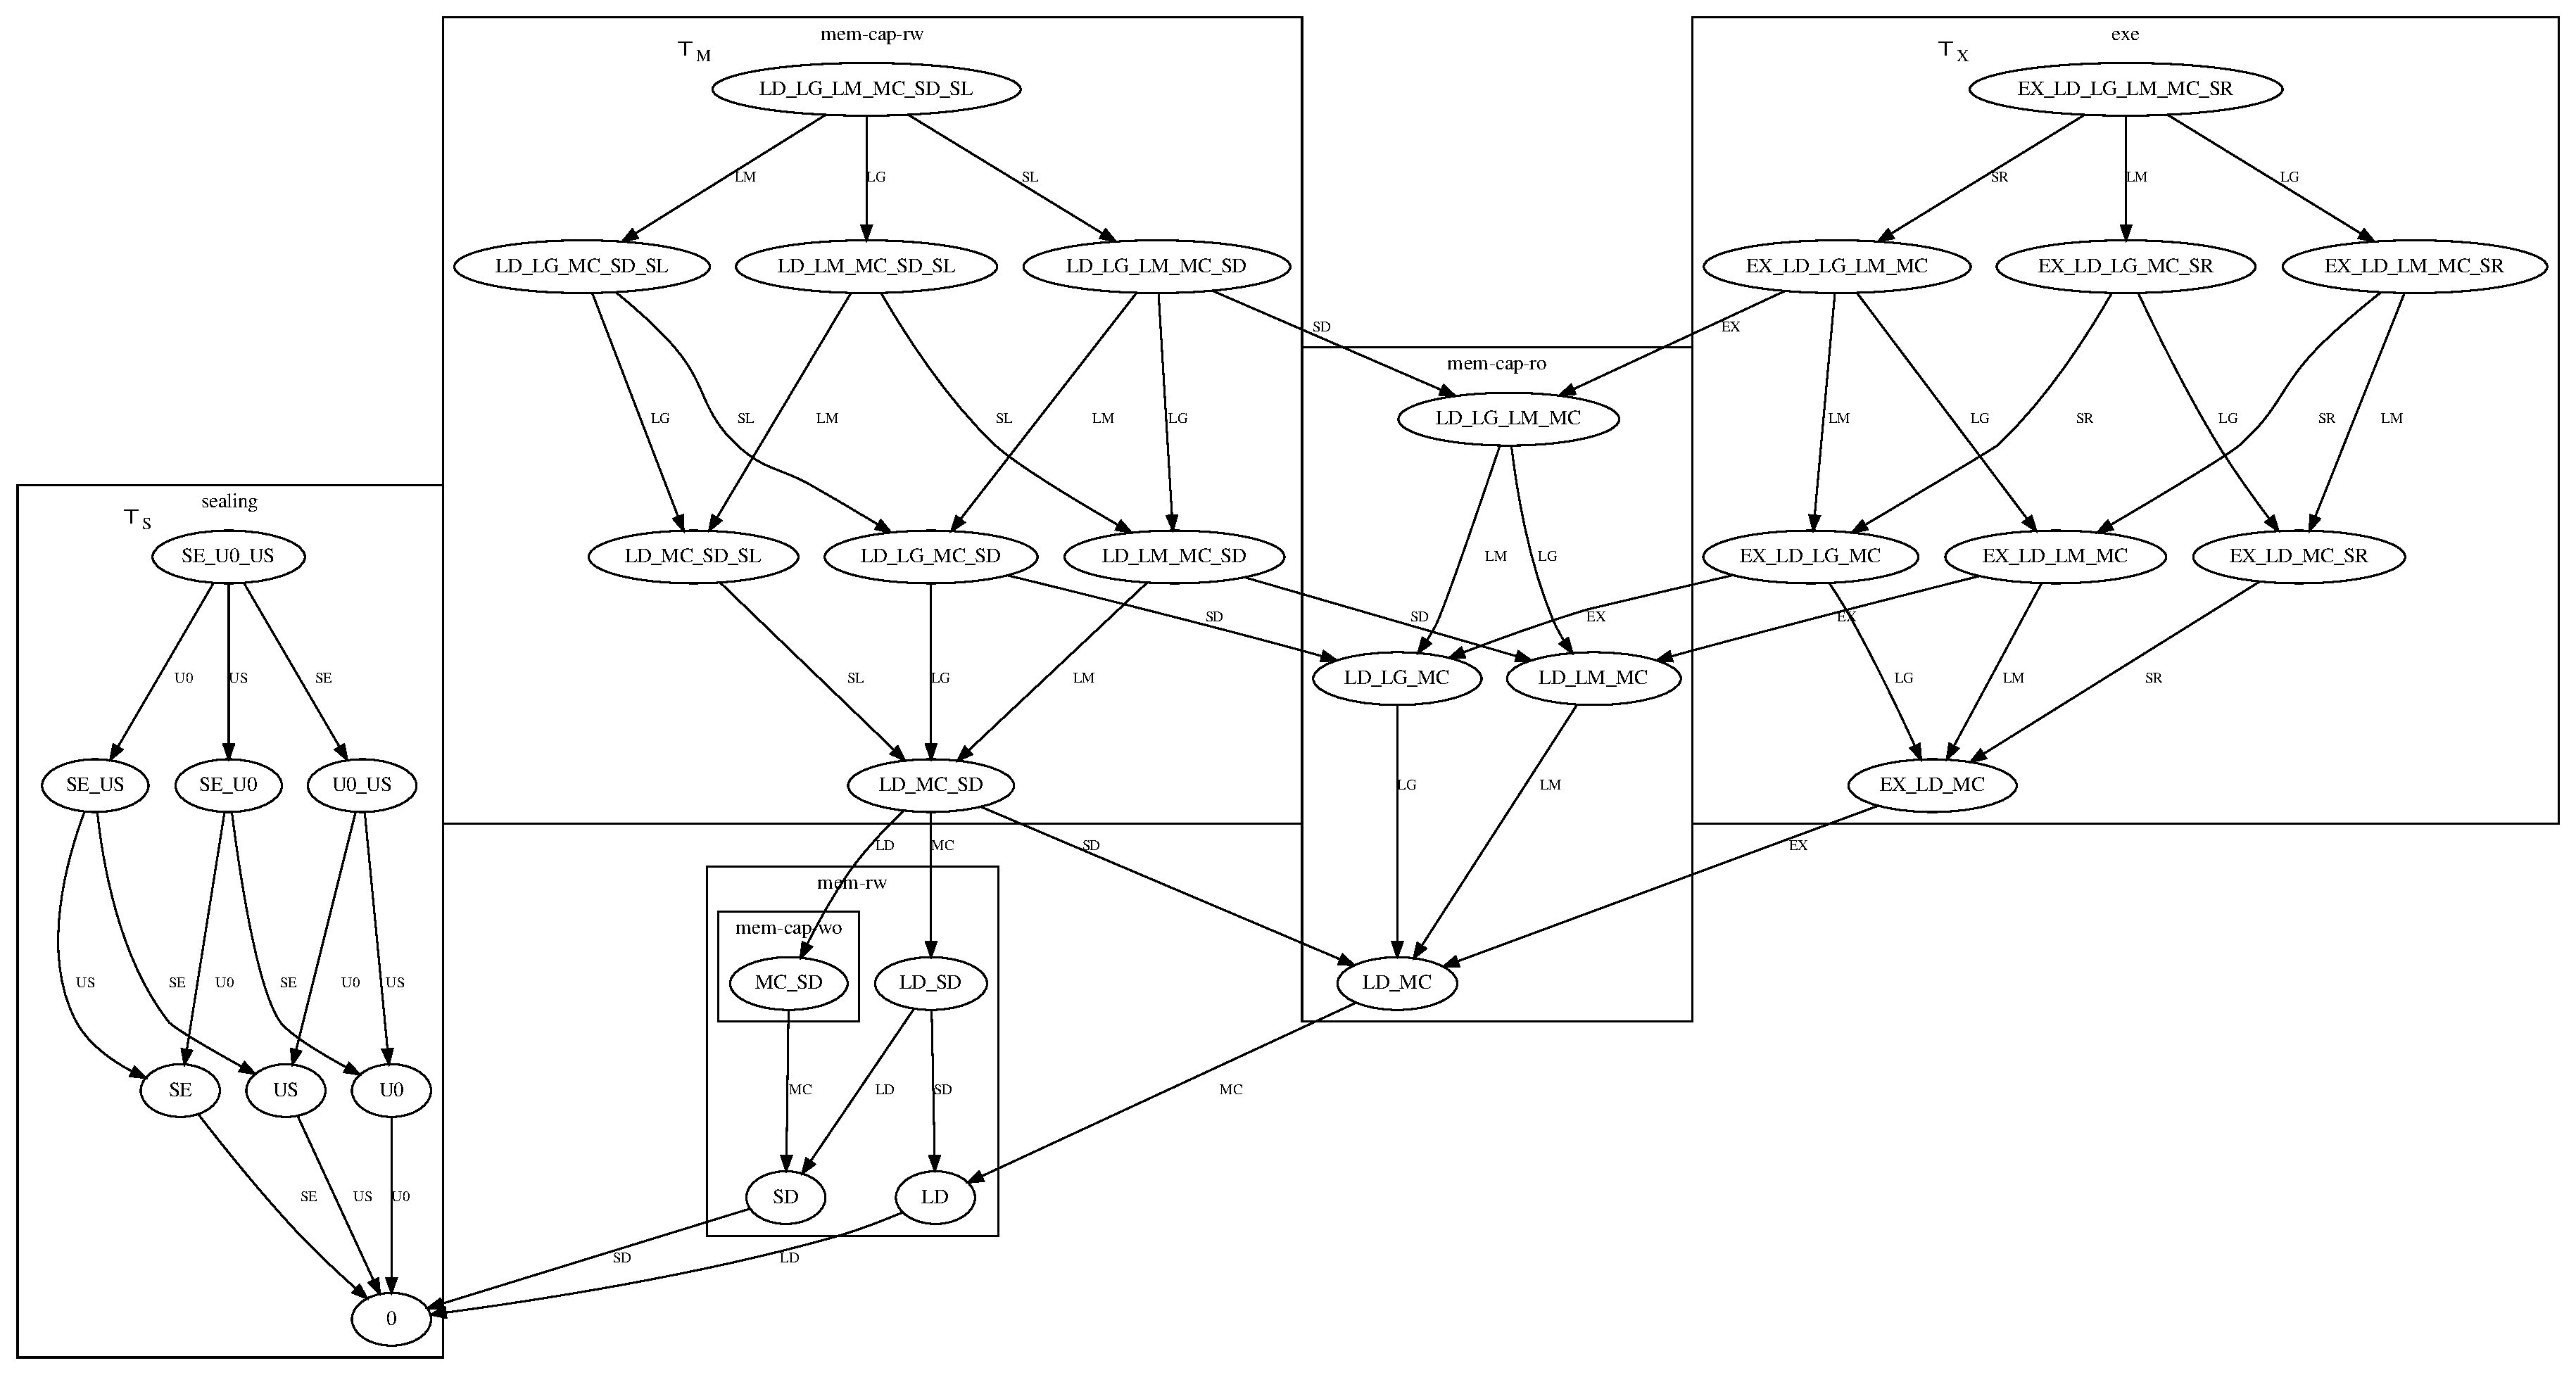
\includegraphics[width=\hsize]{misc/perms/perms5_clustered.pdf}
        \caption{\label{fig:perms5clustered}Graph of allowed permission combinations, grouped by encoding format and ordered by inclusion.
        Edges are labelled with the permission that is dropped by that transition.
        Edges implied by transitivity are omitted. \cappermG is omitted because it is entirely orthogonal.}
    \end{figure}
\end{landscape}
\restoregeometry

\insnriscvref{CAndPerm} operates on the decompressed permissions so it is possible to request combinations that cannot be represented in the compressed encoding (for example \cappermX but not \cappermL).
In that case the resulting capability will have a (possibly empty) subset of the requested permissions.
The following procedure is used to encode a given set of requested permissions:
\begin{enumerate}
\item If the permissions include EX, LD and MC then encode SR, LM and LG using the executable format.
\item Otherwise, if the permissions include LD, MC and SD then encode SL, LM and LG using the cap-read-write format.
\item Otherwise, if the permissions include LD and MC then encode LM and LG using the cap-read-only format.
\item Otherwise, if the permissions include SD and MC then encode using the cap-write-only format.
\item Otherwise, if the permissions include LD \emph{or} SD then encode using the data-only format.
\item Otherwise, encode U0, SE and US using the sealing format.
\end{enumerate}
Any permissions that cannot be encoded using the chosen format are dropped.
The possible clearing of GL and LG or SD and LM during capability loads can be quite easily performed on the compressed format although note that clearing SD may require switching format and that SL may be cleared as a side-effect.

Note that this legalization of permissions must happen at all points where permissions can change (\insnriscvref{CAndPerm} and \insnriscvref{CLC}).
For example, the result of \asm{CAndPerm} followed by \asm{CGetPerm} should be consistent regardless of whether the register file stores the permissions in the compressed or decompressed form.
Similarly, storing then loading a capability should not change the permissions except possibly GL, LG, LM and SD as specified by \insnriscvref{CLC}.


\subsection{Sealed capabilities}
\label{sec:sealing}
The \cotype{} field is used for \emph{sealing} capabilities.
A sealed capability cannot be modified or used as authority for operations except special unsealing ones, but can be passed as a token and later unsealed.
Two kinds of sealing are supported:

\begin{description}
  \item[Using otypes:] \insnriscvref{CSeal} allows the creation of sealed capabilities with a given value of \cotype{} given a capability to seal and an authorizing capability with \cappermSeal and the address set to the desired \cotype{}.
   \insnriscvref{CUnseal} permits unsealing a sealed capability if provided with a capability with \cappermUnseal and bounds that contain the \cotype{} of the capability to be unsealed.
  \item[Sealed entry capabilities (sentries):] Executable capabilities sealed with the special \emph{sentry} \cotype{}s can be used with \insnriscvref{CJALR}.
  The capability is unsealed before jumping to it, creating a form of call gate.
  Three kinds of sentry are defined that affect \asm{mstatus.MIE} in different ways: either leaving it unchanged, enabling interrupts or disabling interrupts.
  Jumping to an interrupt enabling or disabling sentry will set or clear \asm{mstatus.MIE} accordingly.
  Additionally, the link register stored by \insnriscvref{CJAL} and \insnriscvref{CJALR} is sealed as a sentry with the current interrupt status: if MIE is set it will produce an interrupt enabling sentry and if it is cleared it will produce an interrupt disabling sentry.
\end{description}
The \cotype{} field uses the following values:
\begin{description}
  \item[0] unsealed
  \item[1] sealed as sentry
  \item[2] sealed as interrupt disabling sentry
  \item[3] sealed as interrupt enabling sentry
  \item[4-5] reserved for use as return sentries in future
  \item[6-7] executable capability sealed with given \cotype{}
  \item[8] reserved (due to encoding)
  \item[9-15] non-executable capability sealed with given \cotype{}
\end{description}
The \cotype{}s $1-7$ can only be applied to executable capabilities, while memory and sealing format capabilities can only be sealed with \cotype{}s $9-15$.
If the \cotype{} field of a memory or sealing format capability is non-zero then bit 3 is implicitly set i.e. \cotype{}s $9-15$ are encoded using values $1-7$.
An attempt to use \insnriscvref{CSeal} or \insnriscvref{CUnseal} with a reserved \cotype{}, or with an \cotype{} not applicable to the capability format, will clear the capability tag.

\subsection{Capability bounds}
\label{sec:bounds}

The capability bounds (\cbase{} and \ctop{}) are stored in a compressed format relative to the \caddress{}, similar to CHERI Concentrate~\cite{Woodruff2019}.
The floating point encoding stores $2^e$-aligned bounds, where $e$ is the exponent.
An exponent of zero can express bounds with byte precision but limits the maximum length of the range to 511 bytes.
Larger exponent values can represent larger ranges, but require more aligned bounds.

To form the \cbase{} and \ctop{} the 9-bit $B$ and $T$ fields from the encoding are inserted into the address at bit $e$ as follows:

\begin{center}
% spread out the table a bit otherwise it is too tight for maths
{
\renewcommand{\arraystretch}{1.5}
\begin{tabular}{r|c|c|c|}
\cline{2-4}
address, $a =$ & $a_\text{top} = a[31:e+9]$ & $a_\text{mid} = a[e+8:e]$  & $a_\text{low} = a[e-1:0]$ \\ \cline{2-4}
base, $b =$    & $a_\text{top}+c_\text{b}$   & $B $ & $0$ \\ \cline{2-4}
top, $t =$     & $a_\text{top}+c_\text{t}$   & $T $ & $0$ \\ \cline{2-4}
\end{tabular}
}
\end{center}

where the top bits of the address are `corrected' according to the following formulae:

\begin{center}
\begin{tabular}{r c l p{1em} r c l}
$c_b$ & = & $\begin{cases}
-1, & \text{if } a_\text{mid} < B \\
0,  & \text{otherwise}
\end{cases}$ 
&&
$c_t$ & = & $\begin{cases}
  -1, & \text{if } a_\text{mid} < B \text{ and } T \ge B \\
  1,  & \text{if } a_\text{mid} \ge B \text{ and } T < B \\
  0,  & \text{otherwise}
\end{cases}$
\end{tabular}
\end{center}

These corrections ensure that the decoded bounds remain the same provided the address is in $[b, b + 2^{e+9})$, the so-called \emph{representable range}.
They work by testing for conditions that indicate whether the \ctop{} and \caddress{} are in the same $2^{e+9}$ aligned region as \cbase{}.
The representable range spans two such regions (one if $B = 0$), which we will call the lower and upper regions, with $b$ always lying in the lower region.
The ISA is constructed to ensure that, for valid capabilities, $a$ and $t$ are in the representable range and $b \le t$.
Therefore if $a_{mid} \lt B$ then $a$ must be in the upper region, where the $a_{top}$ bits are one greater than those bits in $b$.
Similarly if $T \lt B$ then $t$ must lie in the upper region and we can compute the necessary correction based on whether $a$ also lies in the upper region.
To maintain the necessary invariant for this to work \insnriscvref{CSetAddr} and \insnriscvref{CIncAddr} clear the \ctag{} if the \caddress{} to goes outside the representable range (see \cref{sec:repcheck}).

In order to permit the format to represent a range covering the entire address space using only a 4-bit exponent there is a special case when $E$ has its maximum value.
The effective exponent, $e$, is defined as:

\begin{center}
\begin{tabular}{r c l}
$e$ &=& $ \begin{cases}
              24,& \text{if } E = 15 \\
              E,& \text{otherwise}
\end{cases} $ \\
\end{tabular}
\end{center}

Thus the root memory capability has $B =$ 0, $T =$ 0x100, $E = 15$ and decodes to the range $[0,2^{32})$.
Note that the decoded top is actually a 33-bit value to accommodate this.

\begin{table}
  \centering
  \begin{tabular}{lrr}
  \toprule
  e  &  alignment, $2^e$ &  maximum length, $511 \times 2^e$ \\
  \midrule
  0  &          1 &         511 \\
  1  &          2 &        1,022 \\
  2  &          4 &        2,044 \\
  3  &          8 &        4,088 \\
  4  &         16 &        8,176 \\
  5  &         32 &       16,352 \\
  6  &         64 &       32,704 \\
  7  &        128 &       65,408 \\
  8  &        256 &      130,816 \\
  9  &        512 &      261,632 \\
  10 &       1,024 &      523,264 \\
  11 &       2,048 &     1,046,528 \\
  12 &       4,096 &     2,093,056 \\
  13 &       8,192 &     4,186,112 \\
  14 &      16,384 &     8,372,224 \\
  24 &   16,777,216 &  8,573,157,376 \\
  \bottomrule
  \end{tabular}
  \caption{\label{tab:caplen}
  Capability bounds alignment and maximum length by exponent value.
  Note that for $e=24$ the maximum length exceeds the size of the address space.
  The length of the root capabilities is $2^{32} = 4,294,967,296$ so no valid capability will ever exceed this length.
  }
\end{table}

\subsection{Set bounds operation}
The \insnriscvref{CSetBounds} instruction must select values for $E$, $B$, and $T$ that encode a requested range defined by a given base, $b$, and length, $l$.
In the case that the requested range is not precisely representable \cbase{} is rounded down and \ctop{} up to multiples of $2^e$, where $e$ is the chosen exponent.
For maximum bounds precision, we desire the the smallest $e$ that can represent the requested region.
From the encoding we can observe that the largest encodable length for a given $e$ is given by $2^e \times (2^9 - 1)$.
Therefore we require a solution to the inequality:
\[
\begin{array}{r c l l}
l & \le & 2^e \times (2^9 - 1)\\
l & \le & 2^{e+9} - 2^e\\
l & \le & 2^{e+9} & \text{approximation}\\
\log_2 l & \le & e+9 \\
\lfloor \log_2 l \rfloor & \le & e + 9 & \text{approximation} \\
\msb(l) & \le & e + 9 & \text{index of most significant set bit is floor of } \log_2 \\
32 - \clz(l) & \le & e + 9 & \text{also expressible as count leading zeros for 32-bit length} \\
23 - \clz(l) & \le & e \\
e & = & 23 - \clz(l) & \text{since we require the smallest e} \\
\end{array}
\]
Since $e$ must be greater than or equal to zero the count leading zeros should be limited to the top 23 bits of $l$ (lengths smaller than 9-bits are expressed with $e = 0$).
% To ensure there is some representable buffer and to accommodate rounding we increment the chosen exponent by one if the length is close to the maximum representable:
% \[
% e' =
% \begin{cases}
% e + 1,\text{ if }l[e+8:e+1] = \text{\asm{0xff}} \\
% e,\text{ otherwise}
% \end{cases}
% \]
Since the exponent is limited to 4-bits, exponents greater than 14 are mapped to the special maximum exponent, 24, which is encoded as 15:
\[
e'=
\begin{cases}
  e,\text{ if } e \le 14 \\
  24,\text{ otherwise}
\end{cases}
\]
Having chosen the exponent, the relevant bits of \cbase{} and \ctop{}, $t = b + l$, are extracted:
\[
  B = b[e' + 9: e'] \hspace{2em} T = t[e' + 9: e']
\]
The bounds are exact if the bits below $e'$ in both $b$ and $t$ are all zero.
By discarding the lower bits of $b$ the \cbase{} is automatically rounded down to a representable value,
but if the top is not exact then we must round it up by incrementing by one to ensure the encoded range includes the requested top.
Note that the calculated $e'$ was based on the requested length, but having rounded the bounds the resulting length may be larger and may exceed the maximum representable length for $e'$.
To check for this we calculate the encoded length $T - B$ (in units of $2^e$), and compare it with the maximum encodable length, $2^9 - 1$.
Note that $B$ and $T$ above are one bit wider than the encoding can store for this purpose.
If the maximum encodable length is exceeded we increment $e$ by one and recompute $B$ and $T$, this time with a guarantee that the resulting length is encodable.
Finally, the oversized $B$ and $T$ can drop their extra most significant bit in the final encoding.
\subsection{Representability checks}
\label{sec:repcheck}

To enable capabilities to be used to implement pointers in the C language the capability encoding is designed to allow the \caddress{} to vary within a limited range without changing the decoded bounds.
The \emph{representable range} of a capability is the set of addresses for which the decoded bounds remain the same.
We also wish to maintain the \emph{monotonicity} invariant that the bounds of a valid capability must be a subset of the bounds of the valid capability from which it is derived.
Therefore, whenever the \caddress{} of a capability changes the hardware must check whether the new address remains within the representable range, otherwise the new bounds would violate this invariant.
For example, if \insnriscvref{CSetAddr} or \insnriscvref{CIncAddr} detects that the new \caddress{} is outside of the representable range then the \ctag{} of the result is cleared.

The representation guarantees that the bounds remain decodable provided the address, $a$, and base, $b$, satisfy $b \le a$ and $a \lt b + 2^{e+9}$.
Additionally, if $e$ is 24 then all addresses are representable.
The representable range always includes \ctop{}, although in some cases it is the highest representable address.
Therefore the representation meets the C-language requirement that pointers may range within object bounds or `one byte past the end'.
Other CHERI implementations include much larger representable ranges than this minimum in order to accommodate common C programming practices.
However, this comes at the cost of bits in the representation and our experience so far has shown that it is not necessary for embedded systems.

The following instructions all set the capability \caddress{} and therefore require a representability check:
\begin{itemize}
  \item \insnriscvref{AUIPCC}
  \item \insnriscvref{AUICGP}
  \item \insnriscvref{CSetAddr}
  \item \insnriscvref{CIncAddr}
\end{itemize}
Note that although \insnriscvref{CJAL} and \insnriscvref{CJALR} also set the address on the link register, it is guaranteed to be representable because its \caddress{} can be at most equal to \PCC{}.\ctop{} given that the jump itself is in bounds.
Therefore no representability check is required for these instructions.

Bounds exceptions on instruction fetch might result in an unrepresentable \MEPCC{}.
To simplify hardware while preserving capability monotonicity the tag of \MEPCC{} is always cleared on instruction fetch bounds violations.
This unrepresentability might mean that the decoded bounds of \MEPCC{} do not match the bounds of \PCC{} at the time of the exception,
but \MEPCC{}.\caddress{} will contain the address of the faulting instruction or instruction fetch.

Validation of \MTCC{} and \MEPCC{} in \insnriscvref{CSpecialRW} prevents potential unrepresentability due to the legalisation of \asm{mtvec} and \asm{mepc}.
To simplify hardware these special registers are validated on write, with violations clearing the tag of the value stored (\cref{sec:scrs}).

\subsection{The NULL capability}
\label{sec:null}

The NULL capability is defined as an untagged capability with an \caddress{} of zero and an encoding of all zeroes.
This definition is for maximum compatibility with the C language, where it is used to represent NULL pointers.
The NULL capability is also used as the value of the \asm{\$c0} register and to store integer results by setting the \caddress{} to the required value.
Although capability fields other than the \caddress{} are not meaningful on untagged capabilities they may be queried using the \asm{CGetX} instructions.
Thus it can be observed that the NULL capability decodes as an untagged, unsealed capability, with no permissions, \cbase{} $0$ and \clength{} $0$\footnote{
  On other CHERI architectures the NULL capability is defined to have maximum length.
  This could be achieved by tweaking the encoding (e.g. by inverting the encoded exponent and making the zero value a special case), but there is no clear advantage to doing this.
}.
Note that NULL-derived capabilities with a non-zero address may have non-zero \cbase{} and \ctop{}, but will be untagged.

\subsection{Zero length capabilities}
\label{sec:zerolengthcaps}

The capability encoding described supports capabilities with zero length, where \cbase{} is equal to \ctop{}.
Such capabilities do not authorize access to any memory (or sealing rights), so it may be tempting to use them as unforgeable tokens (e.g. to implement file handles), however they come with a big drawback:
zero length capabilities can be derived with \cbase{} equal to the \ctop{} of an existing capability, even though that capability does not authorize access to \ctop{}.
To give an example of this suppose a memory allocator gives out two capabilities with adjacent ranges $[a,b)$ and $[b,c)$.
Later it may receive a call to `free' with a zero length capability $[b,b)$ and it has no way to tell which of the two ranges it was derived from.
If it relies only on the \cbase{} of the capability and does not validate the length the allocator may incorrectly free $[b,c)$.
The same problem arises during revocation sweeps as performed by Cornucopia~\cite{cornucopia}, meaning it is unable to revoke zero length capabilities.
Therefore we strongly discourage the use of zero length capabilities and encourage validating the length of untrusted capabilities.
As an alternative we suggest using capabilities of length one derived from the sealing root but without \cappermSeal or \cappermUnseal.
In this case \cappermUZ may be used as a software defined permission.

\TODO{Consider having CSetBounds clear the tag on zero length caps to avoid these problems. This would also be necessary if we moved to an encoding that doesn't allow zero length caps.}

\subsection{Zero permission capabilities}

In a similar vein to zero length capabilities the encoding also supports capabilities with no permissions.
These are encoded using the sealing format but may be derived from any of the roots.
We therefore caution against using zero permission capabilities as tokens, because the ability to derive the same capability from either a memory or a sealing root may break the expected unforgeability property.
They may also behave unexpectedly with respect to revocation, since sealing capabilities are not subject to revocation but memory capabilities are.
Given these limitations it is not clear that zero permission capabilities should be allowed at all and support may be removed in future revisions.

\subsection{Capability layout in memory}

While \cref{fig:capformat} shows the nominal capability format, for microarchitectural reasons it may be preferable for the capability fields to appear in a different arrangement in memory.
Future versions of the architecture may also specify a different capability format.
Therefore software should not rely on the exact layout of capabilities in memory.
This said, we expect that certain software will need knowledge of the capability format.
For example, memory allocators and the toolchain will need to be aware of alignment requirements and a debugger will need to be able to decode capabilities from memory dumps.

\subsection{Sail implementation}

\cref{chap:sailenc} contains Sail code implementing the capability
encoding described here as well as properties validated using SMT.

\section{Instruction compression}
\label{sec:c-extension}

Compressed load and store extensions from the standard RV32 C extension decompress to their capability equivalents.
Similar to the encodings of \insnriscvref{CLC} and \insnriscvref{CSC} in uncompressed instructions, the C extension uses compressed \asm{C.LD} and \asm{C.SD} from RV64 to encode \insnriscvref{CLC} and \insnriscvref{CSC}.
In RV32 these opcodes are used to encode \asm{C.FLW} and \asm{C.FSW}, meaning these compressed encodings for floating point loads and stores are no longer available.
Note that this applies to C instructions with implicit stack operands, that is we use \asm{C.LDSP} (RV64) and \asm{C.SDSP} (RV64) as capability loads and stores relative to the stack capability, replacing the \asm{C.FLWSP} (RV32) and \asm{C.FSWSP} (RV32) encodings.
Such a decision is justified because capability loads and stores greatly outnumber floating point instructions in embedded code, and most devices this ISA is targeting do not have a floating point unit at all.

Implicit stack pointer arithmetic instructions are not useful with CHERI, as adding an offset with \asm{ADD} will produce an untagged integer.
These instructions are modified to decode to \insnriscvref{CIncAddr} to produce valid stack-derived capabilities.
As a result, \asm{C.ADDI16SP imm} is decoded into \asm{CIncAddr \$csp, \$csp, imm} and \asm{C.ADDI4SPN \$rd, imm} into \asm{CIncAddr \$cd, \$csp, imm}.

The \cherimcuisa{} introduces changes to mappings between certain compressed and uncompressed instructions, but no changes to the encodings of compressed instructions themselves.
This translates to minimum logic modifications when adding \cherimcuisa{} support to an existing RISC-V CPU.
However, experiments in \cref{chap:c-changes} show that further code size reduction can be achieved by introducing changes in the encoding themselves, to accommodate RV32E and CHERI instructions.

{
\setlength{\parindent}{0cm}

\ifcsname @def@riscv@insns@tex\endcsname
  \ea\endinput
\fi
\ea\gdef\csname @def@riscv@insns@tex\endcsname{1}

\ifcsname @def@riscv@insns@macros@tex\endcsname
  \ea\endinput
\fi
\ea\gdef\csname @def@riscv@insns@macros@tex\endcsname{1}

\makeatletter
% class func name tablestr
\newcommand{\@rvcheriencdef}[4]{%
  \ea\ifx\csname @rvcheri@enc@func2name@#1@\the\numexpr(#2)\endcsname\relax%
    \csgdef{@rvcheri@enc@func2name@#1@\the\numexpr(#2)}{#3}%
    \csgdef{@rvcheri@enc@func2tablestr@#1@\the\numexpr(#2)}{#4}%
  \else%
    \def\@rvcheriencdef@duperror##1{%
      \GenericError{[RISC-V (#1)] }{Duplicate encoding}{%
        [RISC-V (#1)] Function code 0x##1 for #3\MessageBreak%
        is already assigned to \csname @rvcheri@enc@func2name@#1@\the\numexpr(#2)\endcsname%
      }{}%
    }%
    \ea\@rvcheriencdef@duperror\ea{\hex{\the\numexpr(#2)}}%
  \fi%
}
\newcommand{\@rvcheriencusetablestr}[2]{\csuse{@rvcheri@enc@func2tablestr@#1@\the\numexpr(#2)}}
\newcommand{\@rvcherimakeencusetablestrcmd}[1]{%
  \ea\newcommand\csname @rvcheriencusetablestr@#1\endcsname[1]{%
    \@rvcheriencusetablestr{#1}{##1}%
  }%
}
\@rvcherimakeencusetablestrcmd{top}
\@rvcherimakeencusetablestrcmd{srcsrcdest}
\@rvcherimakeencusetablestrcmd{srcsrc}
\@rvcherimakeencusetablestrcmd{src}
\@rvcherimakeencusetablestrcmd{srcdest}
\@rvcherimakeencusetablestrcmd{dest}
\@rvcherimakeencusetablestrcmd{expload}
\@rvcherimakeencusetablestrcmd{expstore}

\let\@rvcherisubclass@tablesuffix\@empty
\define@key{@rvcherisubclass}{tablesuffix}{\def\@rvcherisubclass@tablesuffix{#1}}
\newcommand{\rvcherisubclass}[4][]{{%
  \setkeys{@rvcherisubclass}{#1}%
  \def\@rvcheriencdef@partial##1{\@rvcheriencdef{#2}{"#3}{#4}{#4##1}}%
  \ea\@rvcheriencdef@partial\ea{\@rvcherisubclass@tablesuffix}%
}}

\newbool{@rvcheri@header}
\newcommand{\rvcheriheader}{\booltrue{@rvcheri@header}}
\newcommand{\@rvcheri@ifheader}[1]{%
  \ifbool{@rvcheri@header}{%
    \global\boolfalse{@rvcheri@header}%
    #1%
  }{}%
}
\newcommand{\@rvcherisrcsrcdest}[4]{
  \begin{bytefield}{32}
    \@rvcheri@ifheader{%
      \bitheader[endianness=big]{0,6,7,11,12,14,15,19,20,24,25,31}\\
    }%
    \bitbox{7}{#1}
    \bitbox{5}{#4}
    \bitbox{5}{#3}
    \bitbox{3}{0x0}
    \bitbox{5}{#2}
    \bitbox{7}{0x5b}
  \end{bytefield}%
}
\newcommand{\@rvcherisrcsrcdestimm}[4]{
  \begin{bytefield}{32}
    \@rvcheri@ifheader{%
      \bitheader[endianness=big]{0,6,7,11,12,14,15,19,20,31}\\
    }%
    \bitbox{12}{#4[11:0]}
    \bitbox{5}{#3}
    \bitbox{3}{#1}
    \bitbox{5}{#2}
    \bitbox{7}{0x5b}
  \end{bytefield}%
}
\newcommand{\@rvcherisrcsrcdestclear}[4]{
  \begin{bytefield}{32}
    \@rvcheri@ifheader{%
      \bitheader[endianness=big]{0,6,7,11,12,14,15,17,18,19,20,24,25,31}\\
    }%
    \bitbox{7}{#1}
    \bitbox{5}{#4}
    \bitbox{2}{#3}
    \bitbox{3}{#2$_{[7:5]}$}
    \bitbox{3}{0x0}
    \bitbox{5}{#2$_{[4:0]}$}
    \bitbox{7}{0x5b}
  \end{bytefield}%
}

\newcommand{\@rvcherisrcsrc}[3]{\@rvcherisrcsrcdest{0x7e}{#1}{#2}{#3}}
\newcommand{\@rvcherisrc}[2]{\@rvcherisrcsrc{0x1f}{#2}{#1}}
\newcommand{\@rvcherisrcdest}[3]{\@rvcherisrcsrcdest{0x7f}{#2}{#3}{#1}}
\newcommand{\@rvcheridest}[2]{\@rvcherisrcdest{0x1f}{#2}{#1}}
\newcommand{\@rvcheriscr}[4]{\@rvcherisrcsrcdest{#1}{#2}{#4}{#3}}
\newcommand{\@rvchericlear}[1]{\@rvcherisrcsrcdestclear{0x7f}{m}{q}{#1}}
\newcommand{\@rvcheristorever}[3]{\@rvcherisrcsrcdest{0x7e}{#1}{#3}{#2}}
\newcommand{\@rvcheriexpload}[3]{\@rvcherisrcsrcdest{0x7d}{#2}{#3}{#1}}
\newcommand{\@rvcheriexpstore}[3]{\@rvcherisrcsrcdest{0x7c}{#1}{#3}{#2}}
\newcommand{\@rvcheriexpstorecond}[4]{\@rvcherisrcsrcdest{0x7c}{#1}{#4}{#2/#3}}

\newcommand{\@rvcheriasmdef}[2]{%
  \ea\ifx\csname @rvcheri@asm@#1\endcsname\relax%
    \csgdef{@rvcheri@asm@#1}{#2}%
  \else%
    \def\@rvcheriasmdef@duperror##1{%
      \GenericError{[RISC-V] }{Duplicate assembly ID}{%
        [RISC-V] Instruction ID ##1 already has an assembly definition%
      }%
    }%
    \@rvcheriasmdef@duperror{#1}%
  \fi%
}

\newcommand{\@rvcheriasmencdef}[3]{%
  \ifthenelse{\equal{\@rvcheriinsn@noref}{true}}{%
    \def\@rvcheriasmencdef@insnref{rvcheriasminsnnoref}%
  }{%
    \def\@rvcheriasmencdef@insnref{rvcheriasminsnref}%
  }%
  \ifthenelse{\equal{\@rvcheriinsn@name}{}}{%
  }{%
    \ea\def%
      \ea\@rvcheriasmencdef@asm@partial%
      \ea##\ea1%
      \ea{%
        \csname rvcheriasmfmt\ea\ea\ea\endcsname%
          \ea\ea\ea[\ea\@rvcheriinsn@restriction\ea]\ea{%
            \csname\@rvcheriasmencdef@insnref\endcsname{##1} #3}}%
    \ea\ea\ea\def%
      \ea\ea\ea\@rvcheriasmencdef@asm%
      \ea\ea\ea{%
        \ea\@rvcheriasmencdef@asm@partial%
        \ea{\@rvcheriinsn@name}}%
    \ea\ea\ea\@rvcheriasmdef\ea\ea\ea{\ea\@rvcheriinsn@id\ea}\ea{\@rvcheriasmencdef@asm}%
    \ifthenelse{\equal{\@rvcheriinsn@id}{\@rvcheriinsn@shortid}}{%
    }{%
      \ea\ea\ea\@rvcheriasmdef\ea\ea\ea{\ea\@rvcheriinsn@shortid\ea}\ea{\@rvcheriasmencdef@asm}%
    }%
    \ifthenelse{\equal{\@rvcheriinsn@notable}{true}}{%
    }{%
      \def\@rvcheriasmencdef@rvcheriencdef@partial{\@rvcheriencdef{#1}{#2}}%
      \ea\def\ea\@rvcheriasmencdef@hypershortname\ea{%
        \csname\@rvcheriasmencdef@insnref\ea\endcsname\ea*\ea{\@rvcheriinsn@shortname}%
      }%
      \ea\ea\ea\def\ea\ea\ea\@rvcheriasmencdef@tablestr\ea\ea\ea{%
        \ea\@rvcheriasmencdef@hypershortname\@rvcheriinsn@tablesuffix%
      }%
      \ea\ea\ea\@rvcheriasmencdef@rvcheriencdef@partial%
        \ea\ea\ea{%
          \ea\@rvcheriinsn@name%
        \ea}%
        \ea{%
          \ea\unexpanded\ea{\@rvcheriasmencdef@tablestr}%
        }%
    }%
  }%
}

\let\@rvcheriinsn@name\@empty
\def\@rvcheriinsn@noref{false}
\def\@rvcheriinsn@notable{false}
\def\@rvcheriinsn@rawfunc{false}
\let\@rvcheriinsn@tablesuffix\@empty
\define@key{@rvcheriinsn}{name}{\def\@rvcheriinsn@name{#1}}
\define@key{@rvcheriinsn}{noref}[true]{\def\@rvcheriinsn@noref{#1}}
\define@key{@rvcheriinsn}{notable}[true]{\def\@rvcheriinsn@notable{#1}}
\define@key{@rvcheriinsn}{rawfunc}[true]{\def\@rvcheriinsn@rawfunc{#1}}
\define@key{@rvcheriinsn}{restriction}{\def\@rvcheriinsn@restriction{#1}}
\define@key{@rvcheriinsn}{shortname}{\def\@rvcheriinsn@shortname{#1}}
\define@key{@rvcheriinsn}{tablesuffix}{\def\@rvcheriinsn@tablesuffix{#1}}
\def\@rvcheriinsnsetkeys#1{%
  \setkeys{@rvcheriinsn}{#1}%
  \ea\ifx\csname @rvcheriinsn@shortname\endcsname\relax%
    \let\@rvcheriinsn@shortname\@rvcheriinsn@name%
  \fi%
  \ea\ifx\csname @rvcheriinsn@name\endcsname\relax%
  \else%
    \ea\def\ea\@rvcheriinsn@id\ea{\@rvcheriinsn@name}%
    \ea\def\ea\@rvcheriinsn@shortid\ea{\@rvcheriinsn@shortname}%
    \ea\ifx\csname @rvcheriinsn@restriction\endcsname\relax%
      \let\@rvcheriinsn@restriction\@empty%
    \else%
      \ea\ea\ea\def\ea\ea\ea\@rvcheriinsn@id\ea\ea\ea{\ea\@rvcheriinsn@id\ea:\@rvcheriinsn@restriction}%
      \ea\ea\ea\def\ea\ea\ea\@rvcheriinsn@shortid\ea\ea\ea{\ea\@rvcheriinsn@shortid\ea:\@rvcheriinsn@restriction}%
    \fi%
  \fi%
}
\def\@rvcheriinsnfmtfunc#1{%
  \ifthenelse{\equal{\@rvcheriinsn@rawfunc}{true}}{%
    #1%
  }{%
    0x\lowercase{#1}%
  }%
}

\newcommand{\@rvcheribitboxdef@single}[2]{%
  \ea\ifx\csname @rvcheri@bitbox@#1\endcsname\relax%
    \csgdef{@rvcheri@bitbox@#1}{#2}%
  \else%
    \def\@rvcheribitboxdef@duperror##1{%
      \GenericError{[RISC-V] }{Duplicate bitbox ID}{%
        [RISC-V] Instruction ID ##1 already has a bitbox definition%
      }%
    }%
    \@rvcheribitboxdef@duperror{#1}%
  \fi%
}

\newcommand{\@rvcheribitboxdef}[1]{%
  \ea\@rvcheribitboxdef@single\ea{\@rvcheriinsn@id}{#1}%
  \ifthenelse{\equal{\@rvcheriinsn@id}{\@rvcheriinsn@shortid}}{%
  }{%
    \ea\@rvcheribitboxdef@single\ea{\@rvcheriinsn@shortid}{#1}%
  }%
}

\def\@rvcherirawbitbox#1{%
  \csname @rvcheri#1\endcsname%
}
\let\rvcherirawbitbox\@rvcherirawbitbox

\newcommand{\rvcherisrcsrcdest}[5][]{{%
  \@rvcheriinsnsetkeys{#1}%
  \@rvcheribitboxdef{\@rvcherirawbitbox{srcsrcdest}{\@rvcheriinsnfmtfunc{#2}}{#3}{#4}{#5}}%
  \@rvcheriasmencdef{srcsrcdest}{"#2}{#3, #4, #5}%
}}
\newcommand{\rvcherisrcsrcdestimm}[5][]{{%
  \@rvcheriinsnsetkeys{#1}%
  \@rvcheribitboxdef{\@rvcherirawbitbox{srcsrcdestimm}{\@rvcheriinsnfmtfunc{#2}}{#3}{#4}{#5}}%
  \@rvcheriasmencdef{top}{"#2}{#3, #4, #5}%
}}
\newcommand{\rvcherisrcsrc}[4][]{{%
  \@rvcheriinsnsetkeys{#1}%
  \@rvcheribitboxdef{\@rvcherirawbitbox{srcsrc}{\@rvcheriinsnfmtfunc{#2}}{#3}{#4}}%
  \@rvcheriasmencdef{srcsrc}{"#2}{#3, #4}%
}}
\newcommand{\rvcherisrc}[3][]{{%
  \@rvcheriinsnsetkeys{#1}%
  \@rvcheribitboxdef{\@rvcherirawbitbox{src}{\@rvcheriinsnfmtfunc{#2}}{#3}}%
  \@rvcheriasmencdef{src}{"#2}{#3}%
}}
\newcommand{\rvcherisrcdest}[4][]{{%
  \@rvcheriinsnsetkeys{#1}%
  \@rvcheribitboxdef{\@rvcherirawbitbox{srcdest}{\@rvcheriinsnfmtfunc{#2}}{#3}{#4}}%
  \@rvcheriasmencdef{srcdest}{"#2}{#3, #4}%
}}
\newcommand{\rvcheridest}[3][]{{%
  \@rvcheriinsnsetkeys{#1}%
  \@rvcheribitboxdef{\@rvcherirawbitbox{dest}{\@rvcheriinsnfmtfunc{#2}}{#3}}%
  \@rvcheriasmencdef{dest}{"#2}{#3}%
}}

\newcommand{\rvcheriscr}[5][]{{%
  \@rvcheriinsnsetkeys{#1}%
  \@rvcheribitboxdef{\@rvcherirawbitbox{scr}{\@rvcheriinsnfmtfunc{#2}}{#3}{#4}{#5}}%
  \@rvcheriasmencdef{srcsrcdest}{"#2}{#3, #4, #5}%
}}
\newcommand{\rvchericlear}[2][]{{%
  \@rvcheriinsnsetkeys{#1}%
  \@rvcheribitboxdef{\@rvcherirawbitbox{clear}{\@rvcheriinsnfmtfunc{#2}}}%
  \@rvcheriasmencdef{srcdest}{"#2}{q(uarter), m(ask)}%
}}

\newcommand{\rvcheristorever}[4][]{{%
  \@rvcheriinsnsetkeys{#1}%
  \@rvcheribitboxdef{\@rvcherirawbitbox{storever}{\@rvcheriinsnfmtfunc{#2}}{#3}{#4}}%
  \@rvcheriasmencdef{srcsrc}{"#2}{#3, #4}%
}}

\newcommand{\rvcheriexpload}[4][]{{%
  \@rvcheriinsnsetkeys{#1}%
  \@rvcheribitboxdef{\@rvcherirawbitbox{expload}{\@rvcheriinsnfmtfunc{#2}}{#3}{#4}}%
  \@rvcheriasmencdef{expload}{"#2}{#3, #4}%
}}
\newcommand{\rvcheriexploadres}[4][]{{%
  \@rvcheriinsnsetkeys{#1}%
  \@rvcheribitboxdef{\@rvcherirawbitbox{expload}{\@rvcheriinsnfmtfunc{#2}}{#3}{#4}}%
  \@rvcheriasmencdef{expload}{"#2}{#3, #4}%
}}
\newcommand{\rvcheriexpstore}[4][]{{%
  \@rvcheriinsnsetkeys{#1}%
  \@rvcheribitboxdef{\@rvcherirawbitbox{expstore}{\@rvcheriinsnfmtfunc{#2}}{#3}{#4}}%
  \@rvcheriasmencdef{expstore}{"#2}{#3, #4}%
}}
\newcommand{\rvcheriexpstorecond}[5][]{{%
  \@rvcheriinsnsetkeys{#1}%
  \@rvcheribitboxdef{\@rvcherirawbitbox{expstorecond}{\@rvcheriinsnfmtfunc{#2}}{#3}{#4}{#5}}%
  \@rvcheriasmencdef{expstore}{"#2}{#4, #5}%
}}

\newcommand{\rvcheribitbox}[1]{%
  \ea\ifx\csname @rvcheri@bitbox@#1\endcsname\relax%
    \def\rvcheribitbox@unknownerr##1{%
      \GenericError{[RISC-V] }{Unknown bitbox ID}{%
        [RISC-V] Instruction ID ##1 has no known bitbox definition%
      }{}%
    }%
    \rvcheribitbox@unknownerr{#1}%
  \else%
    \csname @rvcheri@bitbox@#1\endcsname%
  \fi%
}

\newcommand{\rvcheriasm}[1]{%
  \ea\ifx\csname @rvcheri@asm@#1\endcsname\relax%
    \def\rvcheriasm@unknownerr##1{%
      \GenericError{[RISC-V] }{Unknown assembly ID}{%
        [RISC-V] Instruction ID ##1 has no known assembly definition%
      }{}%
    }%
    \rvcheriasm@unknownerr{#1}%
  \else%
    \csname @rvcheri@asm@#1\endcsname%
  \fi%
}
\makeatother


\rvcherisubclass{top}{0}{Two Source \& Dest}

\rvcherisubclass{srcsrcdest}{7C}{Stores}
\rvcherisubclass{srcsrcdest}{7D}{Loads}
\rvcherisubclass{srcsrcdest}{7E}{Two Source}
\rvcherisubclass{srcsrcdest}{7F}{Source \& Dest}

\rvcherisubclass{srcsrc}{1F}{One Source}

\rvcherisubclass{srcdest}{1F}{Dest-Only}

\rvcherisrcdest[name=CGetPerm]{0}{rd}{cs1}
\rvcherisrcdest[name=CGetType]{1}{rd}{cs1}
\rvcherisrcdest[name=CGetBase]{2}{rd}{cs1}
\rvcherisrcdest[name=CGetLen]{3}{rd}{cs1}
\rvcherisrcdest[name=CGetTag]{4}{rd}{cs1}
\rvcherisrcdest[name=CGetAddr]{F}{rd}{cs1}
\rvcherisrcdest[name=CGetHigh]{17}{rd}{cs1}
\rvcherisrcdest[name=CGetTop]{18}{rd}{cs1}

\rvcherisrcsrcdest[name=CSeal]{B}{cd}{cs1}{cs2}
\rvcherisrcsrcdest[name=CUnseal]{C}{cd}{cs1}{cs2}
\rvcherisrcsrcdest[name=CAndPerm]{D}{cd}{cs1}{rs2}
\rvcherisrcsrcdest[name=CSetAddr]{10}{cd}{cs1}{rs2}
\rvcherisrcsrcdest[name=CIncAddr]{11}{cd}{cs1}{rs2}
\rvcherisrcsrcdestimm[name=CIncAddrImm]{1}{cd}{cs1}{imm}
\rvcherisrcsrcdest[name=CSetBounds]{8}{cd}{cs1}{rs2}
\rvcherisrcsrcdest[name=CSetBoundsExact]{9}{cd}{cs1}{rs2}
\rvcherisrcsrcdestimm[name=CSetBoundsImm]{2}{cd}{cs1}{uimm}
\rvcherisrcsrcdest[name=CSetHigh]{16}{cd}{cs1}{rs2}
\rvcherisrcdest[name=CClearTag]{B}{cd}{cs1}
% \rvcherisrcsrcdest[name=CRelocate,noref,tablesuffix=\rvcherireservedfootnotemark]{15}{cd}{cs1}{rs2}

\rvcherisrcsrcdest[name=CSub]{14}{rd}{cs1}{cs2}
\rvcherisrcdest[name=CMove]{A}{cd}{cs1}

\rvcherisrcsrcdest[name=CTestSubset]{20}{rd}{cs1}{cs2}
\rvcherisrcsrcdest[name=CSetEqualExact,shortname=CSEQX]{21}{rd}{cs1}{cs2}

\rvcheriscr[name=CSpecialRW]{1}{cd}{scr}{cs1}

\rvcherisrcdest[name=CRoundRepresentableLength,shortname=CRRL]{8}{rd}{rs1}
\rvcherisrcdest[name=CRepresentableAlignmentMask,shortname=CRAM]{9}{rd}{rs1}

% \rvcheriexploadres[name=LR.B.CAP,noref,tablesuffix=\rvcheriatomicfootnotemark]{18}{rd}{cs1}
% \rvcheriexploadres[name=LR.H.CAP,noref,tablesuffix=\rvcheriatomicfootnotemark]{19}{rd}{cs1}
% \rvcheriexploadres[name=LR.W.CAP,noref,tablesuffix=\rvcheriatomicfootnotemark]{1A}{rd}{cs1}
% \rvcheriexploadres[name=LR.C.CAP,restriction=RV32,noref,tablesuffix=\rvcheriatomicfootnotemark,notable]{1B}{cd}{cs1}
% \rvcheriexploadres[name=LR.D.CAP,restriction=RV64/128,noref,tablesuffix=\rvcheriatomicfootnotemark]{1B}{rd}{cs1}
% \rvcheriexploadres[name=LR.C.CAP,restriction=RV64,noref,tablesuffix=\rvcheriatomicfootnotemark,notable]{1C}{cd}{cs1}
% \rvcheriexploadres[name=LR.Q.CAP,restriction=RV128,noref,tablesuffix=\rvcheriatomicfootnotemark]{1C}{rd}{cs1}

% \rvcheriexpstorecond[name=SC.B.CAP,noref,tablesuffix=\rvcheriatomicfootnotemark]{18}{rd}{rs2}{cs1}
% \rvcheriexpstorecond[name=SC.H.CAP,noref,tablesuffix=\rvcheriatomicfootnotemark]{19}{rd}{rs2}{cs1}
% \rvcheriexpstorecond[name=SC.W.CAP,noref,tablesuffix=\rvcheriatomicfootnotemark]{1A}{rd}{rs2}{cs1}
% \rvcheriexpstorecond[name=SC.C.CAP,restriction=RV32,noref,tablesuffix=\rvcheriatomicfootnotemark,notable]{1B}{cd}{cs2}{cs1}
% \rvcheriexpstorecond[name=SC.D.CAP,restriction=RV64/128,noref,tablesuffix=\rvcheriatomicfootnotemark]{1B}{rd}{rs2}{cs1}
% \rvcheriexpstorecond[name=SC.C.CAP,restriction=RV64,noref,tablesuffix=\rvcheriatomicfootnotemark,notable]{1C}{cd}{cs2}{cs1}
% \rvcheriexpstorecond[name=SC.Q.CAP,restriction=RV128,noref,tablesuffix=\rvcheriatomicfootnotemark]{1C}{rd}{rs2}{cs1}

\ifcsname @app@isaquick@table@macros@tex\endcsname
  \ea\endinput
\fi
\ea\gdef\csname @app@isaquick@table@macros@tex\endcsname{1}

\makeatletter
\newcount\@cherienctable@col
\newcount\@cherienctable@cols
\newcount\@cherienctable@colbits
\newcount\@cherienctable@row
\newcount\@cherienctable@rows
\newcount\@cherienctable@rowbits
\newcount\@cherienctable@tmp
\def\@cherienctable@addtoformat#1{\ea\global\ea\def\ea\@cherienctable@format\ea{\@cherienctable@format #1}}
\def\@cherienctable@addtobody#1{\ea\global\ea\def\ea\@cherienctable@body\ea{\@cherienctable@body #1}}
% cols func2str count
\newcommand{\@cherienctable}[3]{%
  \@cherienctable@cols=\numexpr(#1)\relax%
  \@cherienctable@rows=\numexpr(#3+\@cherienctable@cols-1)\relax%
  \divide\@cherienctable@rows\@cherienctable@cols%
  %
  \let\@cherienctable@format\@empty%
  \let\@cherienctable@body\@empty%
  \ifnum\@cherienctable@rows>1%
    \@cherienctable@addtoformat{r|}%
    \@cherienctable@addtobody{ & }%
  \fi%
  %
  \@cherienctable@colbits=1%
  \@cherienctable@tmp=2%
  \loop\ifnum\@cherienctable@tmp<\@cherienctable@cols%
    \advance\@cherienctable@colbits 1%
    \multiply\@cherienctable@tmp 2%
  \repeat%
  %
  \@cherienctable@rowbits=1%
  \@cherienctable@tmp=2%
  \loop\ifnum\@cherienctable@tmp<\@cherienctable@rows%
    \advance\@cherienctable@rowbits 1%
    \multiply\@cherienctable@tmp 2%
  \repeat%
  %
  \@cherienctable@col=0%
  \loop\ifnum\@cherienctable@col<\@cherienctable@cols%
    \@cherienctable@addtoformat{c}%
    \ifnum\@cherienctable@col>0%
      \@cherienctable@addtobody{ & }%
    \fi%
    \edef\@cherienctable@cell{\nbinary{\@cherienctable@colbits}{\the\@cherienctable@col}}%
    \ea\@cherienctable@addtobody\ea{\@cherienctable@cell}%
    \advance\@cherienctable@col 1%
  \repeat%
  \@cherienctable@addtobody{ \\ \hline}%
  %
  \@cherienctable@row=0%
  \loop\ifnum\@cherienctable@row<\@cherienctable@rows%
    \ifnum\@cherienctable@rows>1%
      \edef\@cherienctable@cell{\nbinary{\@cherienctable@rowbits}{\the\@cherienctable@row}}%
      \ea\@cherienctable@addtobody\ea{\@cherienctable@cell & }%
    \fi%
    \@cherienctable@col=0%
    {%
      \loop\ifnum\@cherienctable@col<\@cherienctable@cols%
        \ifnum\@cherienctable@col>0%
          \@cherienctable@addtobody{ & }%
        \fi%
        \edef\@cherienctable@cell{\csname #2\endcsname{\@cherienctable@row*\@cherienctable@cols + \@cherienctable@col}}%
        \ifx\@cherienctable@cell\@empty%
          \@cherienctable@addtobody{-}%
        \else%
          \ea\@cherienctable@addtobody\ea{\@cherienctable@cell}%
        \fi%
        \advance\@cherienctable@col 1%
      \repeat%
    }%
    \@cherienctable@addtobody{ \\}%
    \advance\@cherienctable@row 1%
  \repeat%
  %
  \def\@cherienctable@begintabular{\begin{tabular}}%
  \ea\@cherienctable@begintabular\ea{\@cherienctable@format}%
  \@cherienctable@body%
  \end{tabular}%
}
\makeatother


\makeatletter
\def\rvcherienctablecols{4}
\def\rvcherienctablefontsize{\normalsize}

% class count
\newcommand{\@rvcherimakeenctablecmd}[2]{%
  % [cols]
  \ea\NewDocumentCommand\ea{\csname rvcherienctable#1\endcsname}{o}{%
    \IfValueTF{##1}{%
      \@cherienctable{##1}{@rvcheriencusetablestr@#1}{#2}%
    }{%
      \ea\@cherienctable\ea{\rvcherienctablecols}{@rvcheriencusetablestr@#1}{#2}%
    }%
  }%
}
\@rvcherimakeenctablecmd{top}{8}
\@rvcherimakeenctablecmd{srcsrcdest}{128}
\@rvcherimakeenctablecmd{srcsrc}{32}
\@rvcherimakeenctablecmd{src}{32}
\@rvcherimakeenctablecmd{srcdest}{32}
\@rvcherimakeenctablecmd{dest}{32}
\@rvcherimakeenctablecmd{expload}{32}
\@rvcherimakeenctablecmd{expstore}{32}

\let\rvcheriasminsnref\insnriscvref
\let\rvcheriasminsnnoref\insnnoref
\providecommand{\rvcheriasmfmt}{}
\renewcommand{\rvcheriasmfmt}[2][]{%
  ~\raiseforbf{%
    \textsf{\footnotesize{#2}}%
    \ifthenelse{\equal{#1}{}}{%
    }{%
      ~{\textit{\scriptsize{(#1)}}}%
    }%
  }%
}

\newcommand{\rvcheriisaquick}[1]{%
  \rvcheribitbox{#1}~\rvcheriasm{#1}%
}

\newcommand{\riscvbitboxaq}{\rotateinbitbox{\small aq}}
\newcommand{\riscvbitboxrl}{\rotateinbitbox{\small rl}}
\makeatother


\chapter{Instruction encoding summary}
\label{app:isaquick-riscv}

	\section{Primary new instructions}

		The RISC-V specification reserves 4 major opcodes for extensions: 11 (0xb / 0b0001011), 43 (0x2b / 0b0101011), 91 (0x5b / 0b1011011), and 123 (0x7b / 0b1111011).
		The proposed CHERI encodings use major opcode 0x5b for all capability instructions.

		All register-register operations use the RISC-V R-type or I-type encoding formats.
	\optype{Capability-Inspection}

		\rvcheriheader
		\rvcheriisaquick{CGetPerm}

		\rvcheriisaquick{CGetType}

		\rvcheriisaquick{CGetBase}

		\rvcheriisaquick{CGetLen}

		\rvcheriisaquick{CGetTag}

		\rvcheriisaquick{CGetAddr}

		\rvcheriisaquick{CGetHigh}

		\rvcheriisaquick{CGetTop}

	\optype{Capability-Modification}

		\rvcheriheader
		\rvcheriisaquick{CSeal}

		\rvcheriisaquick{CUnseal}

		\rvcheriisaquick{CAndPerm}

		\rvcheriisaquick{CSetAddr}

		\rvcheriisaquick{CIncAddr}

		\rvcheriisaquick{CIncAddrImm}

		\rvcheriisaquick{CSetBounds}

		\rvcheriisaquick{CSetBoundsExact}

		\rvcheriisaquick{CSetBoundsRoundDown}

		\rvcheriisaquick{CSetBoundsImm}

		\rvcheriisaquick{CSetHigh}

		\rvcheriisaquick{CClearTag}

		\texttt{CSetBoundsExact} may not be required.

	\optype{Pointer-Arithmetic}

		\rvcheriheader

		\jwnote{We do not need CSub, since a standard Sub will return the difference between two capabilities.}

		\jrtcnote{We do need a separate CSub with a split register file though,
		so we define one that should be used even with a merged register file.}

		\rvcheriisaquick{CSub}

		\rvcheriisaquick{CMove}

	\optype{Pointer-Comparison}

		\rvcheriheader

		\rvcheriisaquick{CTestSubset}

		\rvcheriisaquick{CSetEqualExact}

	\optype{Special Capabilty Register Access}
	\rvcheriheader

		\rvcheriisaquick{CSpecialRW}

	\optype{Adjusting to Compressed Capability Precision}
	\rvcheriheader

		\rvcheriisaquick{CRoundRepresentableLength}

		\rvcheriisaquick{CRepresentableAlignmentMask}

	\section{Modifications to existing RISC-V instructions}
	\optype{Control-Flow}

	No special new control flow instructions are added, although RISC-V \texttt{JAL} / \texttt{JALR} become capability instructions \rvcheriasminsnref{CJAL}  / \rvcheriasminsnref{CJALR}.

	\optype{Memory-Access}
	\label{quickref:mem}

	\vspace{1.5ex}

The standard RV32 load and store instructions are modified to take a capability
as the base address:\\

		\begin{bytefield}{32}
			\bitheader[endianness=big]{0,6,7,11,12,14,15,19,20,24,25,31}\\
			\bitbox{12}{imm[11:0]}
			\bitbox{5}{cs1}
			\bitbox{3}{op}
			\bitbox{5}{rd}
			\bitbox{7}{0x3}
		\end{bytefield}
		\rvcheriasmfmt{CL[BHW][U] rd, imm(cs1)}

		\begin{bytefield}{32}
			\bitbox{7}{imm[11:5]}
			\bitbox{5}{rs2}
			\bitbox{5}{cs1}
			\bitbox{3}{op}
			\bitbox{5}{imm[4:0]}
			\bitbox{7}{0x23}
		\end{bytefield}
		\rvcheriasmfmt{CS[BHW] rs2, imm(cs1)}\\

The RV64 instructions \texttt{LD} and \texttt{SD} are reused to behave as load capability (\texttt{LC}) and store capability (\texttt{SC}) respectively:\\

		\begin{bytefield}{32}
			\bitheader[endianness=big]{0,6,7,11,12,14,15,19,20,24,25,31}\\
			\bitbox{12}{imm}
			\bitbox{5}{cs1}
			\bitbox{3}{0x3}
			\bitbox{5}{cd}
			\bitbox{7}{0x3}
		\end{bytefield}
		\rvcheriasmfmt[RV32]{\rvcheriasminsnref{CLC} cd, imm(cs1)}

		\begin{bytefield}{32}
			\bitbox{7}{imm[11:5]}
			\bitbox{5}{cs2}
			\bitbox{5}{cs1}
			\bitbox{3}{0x3}
			\bitbox{5}{imm[4:0]}
			\bitbox{7}{0x23}
		\end{bytefield}
		\rvcheriasmfmt[RV32]{\rvcheriasminsnref{CSC} cs2, imm(cs1)}\\

% 	\optype{Atomic Memory-Access}

% When using 64-bit capabilities in RV32, the RV64A instructions \texttt{LR.D}, \texttt{SC.D} and \texttt{AMOSWAP.D} are reused to behave as \texttt{LR.C}, \texttt{SC.C} and \texttt{AMOSWAP.C} respectively.\\

% 		\begin{bytefield}{32}
% 			\bitheader[endianness=big]{0,6,7,11,12,14,15,19,20,24,25,26,27,31}\\
% 			\bitbox{5}{0x2}
% 			\bitbox{1}{\riscvbitboxaq}
% 			\bitbox{1}{\riscvbitboxrl}
% 			\bitbox{5}{0x0}
% 			\bitbox{5}{rs1}
% 			\bitbox{3}{0x3}
% 			\bitbox{5}{cd}
% 			\bitbox{7}{0x2f}
% 		\end{bytefield}
% 		\rvcheriasmfmt[RV32]{\rvcheriasminsnnoref{LR.C} cd, rs1}

% 		\begin{bytefield}{32}
% 			\bitbox{5}{0x3}
% 			\bitbox{1}{\riscvbitboxaq}
% 			\bitbox{1}{\riscvbitboxrl}
% 			\bitbox{5}{cs2}
% 			\bitbox{5}{rs1}
% 			\bitbox{3}{0x3}
% 			\bitbox{5}{rd}
% 			\bitbox{7}{0x2f}
% 		\end{bytefield}
% 		\rvcheriasmfmt[RV32]{\rvcheriasminsnnoref{SC.C} rd, cs2, rs1}

% 		\begin{bytefield}{32}
% 			\bitbox{5}{0x1}
% 			\bitbox{1}{\riscvbitboxaq}
% 			\bitbox{1}{\riscvbitboxrl}
% 			\bitbox{5}{cs2}
% 			\bitbox{5}{rs1}
% 			\bitbox{3}{0x3}
% 			\bitbox{5}{cd}
% 			\bitbox{7}{0x2f}
% 		\end{bytefield}
% 		\rvcheriasmfmt[RV32]{\rvcheriasminsnnoref{AMOSWAP.C} cd, cs2, rs1}
%
% We do not provide any of the other AMOs at this point when operating on
% capability values, as they generally make sense only when operating on integer
% values.

% Since capabilities have precise bounds, sub-word atomics cannot be implemented
% using word-sized atomics. To avoid unnecessary complexity compared with a
% non-CHERI RISC-V implementation, we define only \texttt{LR.B}, \texttt{SC.B},
% \texttt{LR.H} and \texttt{SC.H}, without any of the corresponding AMOs. We also
% only require these to be present in capability mode, but implementations may
% choose to always provide them for simplicity.

% 		\begin{bytefield}{32}
% 			\bitheader[endianness=big]{0,6,7,11,12,14,15,19,20,24,25,26,27,31}\\
% 			\bitbox{5}{0x2}
% 			\bitbox{1}{\riscvbitboxaq}
% 			\bitbox{1}{\riscvbitboxrl}
% 			\bitbox{5}{0x0}
% 			\bitbox{5}{rs1}
% 			\bitbox{3}{0x0}
% 			\bitbox{5}{rd}
% 			\bitbox{7}{0x2f}
% 		\end{bytefield}
% 		\rvcheriasmfmt{\rvcheriasminsnnoref{LR.B} rd, rs1}

% 		\begin{bytefield}{32}
% 			\bitbox{5}{0x3}
% 			\bitbox{1}{\riscvbitboxaq}
% 			\bitbox{1}{\riscvbitboxrl}
% 			\bitbox{5}{rs2}
% 			\bitbox{5}{rs1}
% 			\bitbox{3}{0x0}
% 			\bitbox{5}{rd}
% 			\bitbox{7}{0x2f}
% 		\end{bytefield}
% 		\rvcheriasmfmt{\rvcheriasminsnnoref{SC.B} rd, rs2, rs1}

% 		\begin{bytefield}{32}
% 			\bitbox{5}{0x2}
% 			\bitbox{1}{\riscvbitboxaq}
% 			\bitbox{1}{\riscvbitboxrl}
% 			\bitbox{5}{0x0}
% 			\bitbox{5}{rs1}
% 			\bitbox{3}{0x1}
% 			\bitbox{5}{rd}
% 			\bitbox{7}{0x2f}
% 		\end{bytefield}
% 		\rvcheriasmfmt{\rvcheriasminsnnoref{LR.H} rd, rs1}

% 		\begin{bytefield}{32}
% 			\bitbox{5}{0x3}
% 			\bitbox{1}{\riscvbitboxaq}
% 			\bitbox{1}{\riscvbitboxrl}
% 			\bitbox{5}{rs2}
% 			\bitbox{5}{rs1}
% 			\bitbox{3}{0x1}
% 			\bitbox{5}{rd}
% 			\bitbox{7}{0x2f}
% 		\end{bytefield}
% 		\rvcheriasmfmt{\rvcheriasminsnnoref{SC.H} rd, rs2, rs1}

\optype{Address Construction}
The \asm{AUIPC} instruction is replaced by \asm{AUIPCC}, which derives capabilities from \PCC{}.
Our ABI also requires a new instruction, \asm{AUICGP}, that is similar to \asm{AUIPCC} but derives from \asm{\$c3} (\asm{\$cgp}).
This required allocating a new major opcode, although we expect that further support for linker relaxation may remove the need for \asm{AUICGP}. \\

	\begin{bytefield}{32}
	\bitheader[endianness=big]{0,6,7,11,12,31}\\
	\bitbox{20}{imm[31:12]}
	\bitbox{5}{cd}
	\bitbox{7}{0x17}
	\end{bytefield}
	\rvcheriasmfmt{\rvcheriasminsnref{AUIPCC} cd, imm}


	\begin{bytefield}{32}
		\bitbox{20}{imm[31:12]}
		\bitbox{5}{cd}
		\bitbox{7}{0x7b}
	\end{bytefield}
	\rvcheriasmfmt{\rvcheriasminsnref{AUICGP} cd, imm}

% 	\section{Assembly Programming}

% 	\subsection{Capability Register ABI Names}

% 	Table~\ref{table:riscv-register-names} lists the ABI names of
% 	the capability registers.  The ABI names follow from the ABI
% 	names of the RISC-V \textbf{x} registers.  All capability registers are
% 	Caller-Save in the hybrid ABI.	Capability registers follow
% 	the same save requirements as \textbf{x} registers in the purecap ABI.

% \begin{table}[h]
% \begin{center}
% \begin{tabular}{lllll}
% \toprule
% Register & ABI Name & Description						& Hybrid Saver & Purecap Saver \\
% \midrule
% c0	& cnull		& NULL pointer					& -		& - \\
% c1	& cra		& Return address					& Caller	& Caller \\
% c2	& csp		& Stack pointer					& Caller	& Callee \\
% c3	& cgp		& Global pointer					& -		& - \\
% c4	& ctp		& Thread pointer					& -		& - \\
% c5	& ct0		& Temporary/alternate link register	& Caller	& Caller \\
% c6-7 & ct1-2		& Temporaries						& Caller	& Caller \\
% c8	& cs0/cfp	& Saved register/frame pointer		& Caller	& Callee \\
% c9	& cs1		& Saved register					& Caller	& Callee \\
% c10-11 & ca0-1	& Function arguments/return values	& Caller	& Caller \\
% c12-17 & ca2-7	& Function arguments				& Caller	& Caller \\
% c18-27 & cs2-11	& Saved registers					& Caller	& Callee \\
% c28-31 & ct3-6	& Temporaries						& Caller	& Caller \\
% \bottomrule
% \end{tabular}
% \end{center}
% \caption{Assembler mnemonics for CHERI RISC-V capability registers}
% \label{table:riscv-register-names}
% \end{table}

% 	\subsection{Capability Encoding Mode Instructions}

% 	Table~\ref{table:riscv-capmode-instructions} lists uncompressed
% 	instructions which change semantics under capability mode.
% 	Table~\ref{table:riscv-capmode-instructions-rvc} lists compressed
% 	instructions which change semantics under capability mode.

% \begin{table}
% \begin{center}
% \begin{tabular}{ll}
% \toprule
% Integer Instruction		& Capability Instruction \\
% \midrule
% \texttt{l\{b|h|w|d\}[u] rd, offset(rs1)} & \texttt{cl\{b|h|w|d\}[u] rd, offset(cs1)} \\
% \texttt{lc cd, offset(rs1)} & \texttt{clc cd, offset(cs1)} \\
% \texttt{s\{b|h|w|d\} rs2, offset(rs1)} & \texttt{cs\{b|h|w|d\} rs2, offset(cs1)} \\
% \texttt{sc rs2, offset(rs1)} & \texttt{csc cs2, offset(cs1)} \\
% \texttt{fl\{h|w|d|q\} fd, offset(rs1)} & \texttt{cfl\{h|w|d|q\} fd, offset(cs1)} \\
% \texttt{fs\{h|w|d|q\} fs2, offset(rs1)} & \texttt{cfs\{h|w|d|q\} fs2, offset(cs1)} \\
% \texttt{lr.\{b|h|w|d\} rd, (rs1)} & \texttt{clr.\{b|h|w|d\} rd, (cs1)} \\
% \texttt{lr.c cd, (rs1)} & \texttt{clr.c cd, (cs1)} \\
% \texttt{sc.\{b|h|w|d\} rd, rs2, (rs1)} & \texttt{csc.\{b|h|w|d\} rd, rs2, (cs1)} \\
% \texttt{sc.c cd, cs2, (rs1)} & \texttt{csc.c cd, cs2, (cs1)} \\
% \texttt{amo<op>.\{w|d\}[.order] rd, rs2, (rs1)} & \texttt{camo<op>.\{w|d\}[.order] rd, rs2, (cs1)} \\
% \texttt{amo<op>.c[.order] cd, cs2, (rs1)} & \texttt{camo<op>.c[.order] cd, cs2, (cs1)} \\
% \texttt{auipc rd, offset} & \texttt{auipcc cd, offset} \\
% \bottomrule
% \end{tabular}
% \end{center}
% \caption{Uncompressed Instructions Dependent on Encoding Mode}
% \label{table:riscv-capmode-instructions}
% \end{table}

% \begin{table}
% \begin{center}
% \begin{tabular}{lll}
% \toprule
% Integer Instruction		& Capability Instruction & ISA \\
% \midrule
% \texttt{c.jr rs1} & \texttt{c.cjr cs1} & - \\
% \texttt{c.jalr rs1} & \texttt{c.cjalr cs1} & - \\
% \texttt{c.l\{w|d\} rd, offset(rs1)} & \texttt{c.cl\{w|d\} rd, offset(cs1)} & - \\
% \texttt{c.l\{w|d\}sp rd, offset(sp)} & \texttt{c.cl\{w|d\}sp rd, offset(csp)} & - \\
% \texttt{c.s\{w|d\} rs2, offset(rs1)} & \texttt{c.cs\{w|d\} rs2, offset(cs1)} & - \\
% \texttt{c.s\{w|d\}sp rs2, offset(sp)} & \texttt{c.cs\{w|d\}sp rs2, offset(csp)} & - \\
% \texttt{c.flw fd, offset(rs1)} & \texttt{c.clc cd, offset(cs1)} & RV32 \\
% \texttt{c.flwsp fd, offset(sp)} & \texttt{c.clcsp cd, offset(csp)} & RV32 \\
% \texttt{c.fsw fs2, offset(rs1)} & \texttt{c.csc cs2, offset(cs1)} & RV32 \\
% \texttt{c.fswsp fs2, offset(sp)} & \texttt{c.cscsp cs2, offset(csp)} & RV32 \\
% \texttt{c.fld fd, offset(rs1)} & \texttt{c.cfld fd, offset(cs1)} & RV32 \\
% \texttt{c.fldsp fd, offset(sp)} & \texttt{c.cfldsp fd, offset(csp)} & RV32 \\
% \texttt{c.fsd fs2, offset(rs1)} & \texttt{c.cfsd fs, offset(cs1)} & RV32 \\
% \texttt{c.fsdsp fs2, offset(sp)} & \texttt{c.cfsdsp fs, offset(csp)} & RV32 \\
% \texttt{c.fld fd, offset(rs1)} & \texttt{c.clc cd, offset(cs1)} & RV64 \\
% \texttt{c.fldsp fd, offset(sp)} & \texttt{c.clcsp cd, offset(csp)} & RV64 \\
% \texttt{c.fsd fs2, offset(rs1)} & \texttt{c.csc cs, offset(cs1)} & RV64 \\
% \texttt{c.fsdsp fs2, offset(sp)} & \texttt{c.cscsp cs, offset(csp)} & RV64 \\
% \bottomrule
% \end{tabular}
% \end{center}
% \caption{Compressed Instructions Dependent on Encoding Mode}
% \label{table:riscv-capmode-instructions-rvc}
% \end{table}

% 	Table~\ref{table:riscv-capmode-pseudo-remove} lists psuedoinstructions
% 	removed in capability mode.
% 	Table~\ref{table:riscv-capmode-pseudo-add} lists psuedoinstructions
% 	added in capability mode.

% \begin{table}
% \begin{center}
% \begin{tabular}{ll}
% \toprule
% Pseudoinstruction	& Meaning \\
% \midrule
% \texttt{la rd, symbol} & Load address \\
% \texttt{lla rd, symbol} & Load local address \\
% \texttt{l\{b|h|w|d\} rd, symbol} & Load global \\
% \texttt{s\{b|h|w|d\} rd, symbol, rt} & Store global \\
% \texttt{fl\{w|d\} rd, symbol, rt} & Floating-point load global \\
% \texttt{fs\{w|d\} rd, symbol, rt} & Floating-point store global \\
% \midrule
% \texttt{call symbol} & Call far-away subroutine \\
% \texttt{tail symbol} & Tail call far-away subroutine \\
% \bottomrule
% \end{tabular}
% \end{center}
% \caption{Pseudoinstructions Removed in Capability Mode}
% \label{table:riscv-capmode-pseudo-remove}
% \end{table}

% \begin{sidewaystable}
% \begin{center}
% \begin{tabular}{lll}
% \toprule
% Pseudoinstruction	& Base Instruction(s)	& Meaning \\
% \midrule
% \texttt{clgc cd, sym} &
%   \begin{tabular}{@{}l@{}}
%   \texttt{1: auipcc cd, \%captab\_pcrel\_hi(sym)} \\ \texttt{\ \ \ \ clc cd, \%pcrel\_lo(1b)(cd)}
%   \end{tabular}
%  & Load from capability table \\
% \texttt{cllc cd, sym} &
%   \begin{tabular}{@{}l@{}}
%   \texttt{1: auipcc cd, \%pcrel\_hi(sym)} \\ \texttt{\ \ \ \ cincoffset cd, cd, \%pcrel\_lo(1b)}
%   \end{tabular}
%  & Load PCC-relative capability \\
% \midrule
% \texttt{cjr cs} & \texttt{cjalr cnull, cs} & Jump to capability \\
% \texttt{cjalr cs} & \texttt{cjalr cra, cs} & Jump to capability and link \\
% \texttt{cret} & \texttt{cjalr cnull, cra} & Return to capability \\
% \midrule
% \texttt{cspecialr cd, scr} & \texttt{cspecialrw cd, scr, cnull} & Read special capability register \\
% \texttt{cspecialw scr, cs} & \texttt{cspecialrw cnull, scr, cs} & Write special capability register \\
% \bottomrule
% \end{tabular}
% \end{center}
% \caption{Pseudoinstructions Added in Capability Mode}
% \label{table:riscv-capmode-pseudo-add}
% % TODO: should the hyperrefs for these pseudos link to CJALR instead?
% \insnriscvlabel{cjr}
% \insnriscvlabel{cret}
% \insnriscvlabel{cspecialr}
% \insnriscvlabel{cspecialw}
% \insnriscvlabel{cllc}
% \insnriscvlabel{clgc}
% \end{sidewaystable}

	\section{Encoding Summary}

	The \cherimcuisa{} shares encodings with CHERI-RISC-V.
	The general-purpose instructions use the 0x5b major opcode and use the RISC-V R-type or I-type encoding formats.
	CHERI-RISC-V uses the funct3 field from bits 14-12 as a top-level opcode, and funct7 as a secondary
	opcode for standard 3-register operand instructions.
	Two-register operand instructions and single-register operand instructions are a subset
	of the 3-register operand encodings.

	\subsection*{Top-level encoding allocation (funct3 field)}
	{\rvcherienctablefontsize
	\rvcherienctabletop
	}

	\subsection*{Two Source \& Dest encoding allocation (funct7 field)}
	All three-register-operand (two sources, one destination) CHERI-RISC-V instructions use the RISC-V R-type encoding format, with the same funct field stored in funct7 and a 0 value in funct3.

	\vspace{1em}

	\rvcherirawbitbox{srcsrcdest}{func}{cd}{cs1}{rs2/cs2}

	\vspace{1em}

	{\rvcherienctablefontsize
	\def\rvcherireservedfootnotemark{$^\dagger$}
	\rvcherienctablesrcsrcdest\\\\
	\footnotesize
	$^\dagger$Reserved for future use.
	}

	\clearpage
	\subsection*{Two Source encoding allocation  (rd field)}
	There are currently no two source instructions but they would be of the following form:
	\vspace{1em}

	\rvcheriheader
	\rvcherirawbitbox{srcsrc}{func}{rs1/cs1}{rs2/cs2}

	\vspace{1em}

	{\rvcherienctablefontsize
	\def\rvcherireservedfootnotemark{$^\dagger$}
	\rvcherienctablesrcsrc\\\\
	\footnotesize
	$^\dagger$Reserved for future use.
	}

	\vspace{1em}

	\subsection*{One Source encoding allocation (rs2 field)}
	There are currently no one source instructions but they would be of the following form:

	\vspace{1em}

	\rvcheriheader
	\rvcherirawbitbox{src}{func}{rs1/cs1}

	\vspace{1em}

	{\rvcherienctablefontsize
	\def\rvcherireservedfootnotemark{$^\dagger$}
	\rvcherienctablesrc\\\\
	\footnotesize
	$^\dagger$Reserved for future use.
	}

	\vspace{1em}

	\subsection*{Source \& Dest encoding allocation (rs2 field)}
	Source \& Dest instructions are of the following form:

	\vspace{1em}

	\rvcheriheader
	\rvcherirawbitbox{srcdest}{func}{rd/cd}{rs1/cs1}

	\vspace{1em}

	{\rvcherienctablefontsize
	\def\rvcherireservedfootnotemark{$^\dagger$}
	\rvcherienctablesrcdest\\\\
	\footnotesize
	$^\dagger$Reserved for future use.
	}

	\vspace{1em}

	\subsection*{Dest-Only encoding allocation (rs1 field)}
	We do not currently have any one-register-operand instructions, but any
	future dest-only instructions will be of the following form:

	\vspace{1em}

	\rvcheriheader
	\rvcherirawbitbox{dest}{func}{rd}

	\vspace{1em}

	{\rvcherienctablefontsize
	\rvcherienctabledest
	}

\chapter{Instruction reference}
\label{chap:isaref-riscv}

\ifcsname @def@riscv@insns@tex\endcsname
  \ea\endinput
\fi
\ea\gdef\csname @def@riscv@insns@tex\endcsname{1}

\ifcsname @def@riscv@insns@macros@tex\endcsname
  \ea\endinput
\fi
\ea\gdef\csname @def@riscv@insns@macros@tex\endcsname{1}

\makeatletter
% class func name tablestr
\newcommand{\@rvcheriencdef}[4]{%
  \ea\ifx\csname @rvcheri@enc@func2name@#1@\the\numexpr(#2)\endcsname\relax%
    \csgdef{@rvcheri@enc@func2name@#1@\the\numexpr(#2)}{#3}%
    \csgdef{@rvcheri@enc@func2tablestr@#1@\the\numexpr(#2)}{#4}%
  \else%
    \def\@rvcheriencdef@duperror##1{%
      \GenericError{[RISC-V (#1)] }{Duplicate encoding}{%
        [RISC-V (#1)] Function code 0x##1 for #3\MessageBreak%
        is already assigned to \csname @rvcheri@enc@func2name@#1@\the\numexpr(#2)\endcsname%
      }{}%
    }%
    \ea\@rvcheriencdef@duperror\ea{\hex{\the\numexpr(#2)}}%
  \fi%
}
\newcommand{\@rvcheriencusetablestr}[2]{\csuse{@rvcheri@enc@func2tablestr@#1@\the\numexpr(#2)}}
\newcommand{\@rvcherimakeencusetablestrcmd}[1]{%
  \ea\newcommand\csname @rvcheriencusetablestr@#1\endcsname[1]{%
    \@rvcheriencusetablestr{#1}{##1}%
  }%
}
\@rvcherimakeencusetablestrcmd{top}
\@rvcherimakeencusetablestrcmd{srcsrcdest}
\@rvcherimakeencusetablestrcmd{srcsrc}
\@rvcherimakeencusetablestrcmd{src}
\@rvcherimakeencusetablestrcmd{srcdest}
\@rvcherimakeencusetablestrcmd{dest}
\@rvcherimakeencusetablestrcmd{expload}
\@rvcherimakeencusetablestrcmd{expstore}

\let\@rvcherisubclass@tablesuffix\@empty
\define@key{@rvcherisubclass}{tablesuffix}{\def\@rvcherisubclass@tablesuffix{#1}}
\newcommand{\rvcherisubclass}[4][]{{%
  \setkeys{@rvcherisubclass}{#1}%
  \def\@rvcheriencdef@partial##1{\@rvcheriencdef{#2}{"#3}{#4}{#4##1}}%
  \ea\@rvcheriencdef@partial\ea{\@rvcherisubclass@tablesuffix}%
}}

\newbool{@rvcheri@header}
\newcommand{\rvcheriheader}{\booltrue{@rvcheri@header}}
\newcommand{\@rvcheri@ifheader}[1]{%
  \ifbool{@rvcheri@header}{%
    \global\boolfalse{@rvcheri@header}%
    #1%
  }{}%
}
\newcommand{\@rvcherisrcsrcdest}[4]{
  \begin{bytefield}{32}
    \@rvcheri@ifheader{%
      \bitheader[endianness=big]{0,6,7,11,12,14,15,19,20,24,25,31}\\
    }%
    \bitbox{7}{#1}
    \bitbox{5}{#4}
    \bitbox{5}{#3}
    \bitbox{3}{0x0}
    \bitbox{5}{#2}
    \bitbox{7}{0x5b}
  \end{bytefield}%
}
\newcommand{\@rvcherisrcsrcdestimm}[4]{
  \begin{bytefield}{32}
    \@rvcheri@ifheader{%
      \bitheader[endianness=big]{0,6,7,11,12,14,15,19,20,31}\\
    }%
    \bitbox{12}{#4[11:0]}
    \bitbox{5}{#3}
    \bitbox{3}{#1}
    \bitbox{5}{#2}
    \bitbox{7}{0x5b}
  \end{bytefield}%
}
\newcommand{\@rvcherisrcsrcdestclear}[4]{
  \begin{bytefield}{32}
    \@rvcheri@ifheader{%
      \bitheader[endianness=big]{0,6,7,11,12,14,15,17,18,19,20,24,25,31}\\
    }%
    \bitbox{7}{#1}
    \bitbox{5}{#4}
    \bitbox{2}{#3}
    \bitbox{3}{#2$_{[7:5]}$}
    \bitbox{3}{0x0}
    \bitbox{5}{#2$_{[4:0]}$}
    \bitbox{7}{0x5b}
  \end{bytefield}%
}

\newcommand{\@rvcherisrcsrc}[3]{\@rvcherisrcsrcdest{0x7e}{#1}{#2}{#3}}
\newcommand{\@rvcherisrc}[2]{\@rvcherisrcsrc{0x1f}{#2}{#1}}
\newcommand{\@rvcherisrcdest}[3]{\@rvcherisrcsrcdest{0x7f}{#2}{#3}{#1}}
\newcommand{\@rvcheridest}[2]{\@rvcherisrcdest{0x1f}{#2}{#1}}
\newcommand{\@rvcheriscr}[4]{\@rvcherisrcsrcdest{#1}{#2}{#4}{#3}}
\newcommand{\@rvchericlear}[1]{\@rvcherisrcsrcdestclear{0x7f}{m}{q}{#1}}
\newcommand{\@rvcheristorever}[3]{\@rvcherisrcsrcdest{0x7e}{#1}{#3}{#2}}
\newcommand{\@rvcheriexpload}[3]{\@rvcherisrcsrcdest{0x7d}{#2}{#3}{#1}}
\newcommand{\@rvcheriexpstore}[3]{\@rvcherisrcsrcdest{0x7c}{#1}{#3}{#2}}
\newcommand{\@rvcheriexpstorecond}[4]{\@rvcherisrcsrcdest{0x7c}{#1}{#4}{#2/#3}}

\newcommand{\@rvcheriasmdef}[2]{%
  \ea\ifx\csname @rvcheri@asm@#1\endcsname\relax%
    \csgdef{@rvcheri@asm@#1}{#2}%
  \else%
    \def\@rvcheriasmdef@duperror##1{%
      \GenericError{[RISC-V] }{Duplicate assembly ID}{%
        [RISC-V] Instruction ID ##1 already has an assembly definition%
      }%
    }%
    \@rvcheriasmdef@duperror{#1}%
  \fi%
}

\newcommand{\@rvcheriasmencdef}[3]{%
  \ifthenelse{\equal{\@rvcheriinsn@noref}{true}}{%
    \def\@rvcheriasmencdef@insnref{rvcheriasminsnnoref}%
  }{%
    \def\@rvcheriasmencdef@insnref{rvcheriasminsnref}%
  }%
  \ifthenelse{\equal{\@rvcheriinsn@name}{}}{%
  }{%
    \ea\def%
      \ea\@rvcheriasmencdef@asm@partial%
      \ea##\ea1%
      \ea{%
        \csname rvcheriasmfmt\ea\ea\ea\endcsname%
          \ea\ea\ea[\ea\@rvcheriinsn@restriction\ea]\ea{%
            \csname\@rvcheriasmencdef@insnref\endcsname{##1} #3}}%
    \ea\ea\ea\def%
      \ea\ea\ea\@rvcheriasmencdef@asm%
      \ea\ea\ea{%
        \ea\@rvcheriasmencdef@asm@partial%
        \ea{\@rvcheriinsn@name}}%
    \ea\ea\ea\@rvcheriasmdef\ea\ea\ea{\ea\@rvcheriinsn@id\ea}\ea{\@rvcheriasmencdef@asm}%
    \ifthenelse{\equal{\@rvcheriinsn@id}{\@rvcheriinsn@shortid}}{%
    }{%
      \ea\ea\ea\@rvcheriasmdef\ea\ea\ea{\ea\@rvcheriinsn@shortid\ea}\ea{\@rvcheriasmencdef@asm}%
    }%
    \ifthenelse{\equal{\@rvcheriinsn@notable}{true}}{%
    }{%
      \def\@rvcheriasmencdef@rvcheriencdef@partial{\@rvcheriencdef{#1}{#2}}%
      \ea\def\ea\@rvcheriasmencdef@hypershortname\ea{%
        \csname\@rvcheriasmencdef@insnref\ea\endcsname\ea*\ea{\@rvcheriinsn@shortname}%
      }%
      \ea\ea\ea\def\ea\ea\ea\@rvcheriasmencdef@tablestr\ea\ea\ea{%
        \ea\@rvcheriasmencdef@hypershortname\@rvcheriinsn@tablesuffix%
      }%
      \ea\ea\ea\@rvcheriasmencdef@rvcheriencdef@partial%
        \ea\ea\ea{%
          \ea\@rvcheriinsn@name%
        \ea}%
        \ea{%
          \ea\unexpanded\ea{\@rvcheriasmencdef@tablestr}%
        }%
    }%
  }%
}

\let\@rvcheriinsn@name\@empty
\def\@rvcheriinsn@noref{false}
\def\@rvcheriinsn@notable{false}
\def\@rvcheriinsn@rawfunc{false}
\let\@rvcheriinsn@tablesuffix\@empty
\define@key{@rvcheriinsn}{name}{\def\@rvcheriinsn@name{#1}}
\define@key{@rvcheriinsn}{noref}[true]{\def\@rvcheriinsn@noref{#1}}
\define@key{@rvcheriinsn}{notable}[true]{\def\@rvcheriinsn@notable{#1}}
\define@key{@rvcheriinsn}{rawfunc}[true]{\def\@rvcheriinsn@rawfunc{#1}}
\define@key{@rvcheriinsn}{restriction}{\def\@rvcheriinsn@restriction{#1}}
\define@key{@rvcheriinsn}{shortname}{\def\@rvcheriinsn@shortname{#1}}
\define@key{@rvcheriinsn}{tablesuffix}{\def\@rvcheriinsn@tablesuffix{#1}}
\def\@rvcheriinsnsetkeys#1{%
  \setkeys{@rvcheriinsn}{#1}%
  \ea\ifx\csname @rvcheriinsn@shortname\endcsname\relax%
    \let\@rvcheriinsn@shortname\@rvcheriinsn@name%
  \fi%
  \ea\ifx\csname @rvcheriinsn@name\endcsname\relax%
  \else%
    \ea\def\ea\@rvcheriinsn@id\ea{\@rvcheriinsn@name}%
    \ea\def\ea\@rvcheriinsn@shortid\ea{\@rvcheriinsn@shortname}%
    \ea\ifx\csname @rvcheriinsn@restriction\endcsname\relax%
      \let\@rvcheriinsn@restriction\@empty%
    \else%
      \ea\ea\ea\def\ea\ea\ea\@rvcheriinsn@id\ea\ea\ea{\ea\@rvcheriinsn@id\ea:\@rvcheriinsn@restriction}%
      \ea\ea\ea\def\ea\ea\ea\@rvcheriinsn@shortid\ea\ea\ea{\ea\@rvcheriinsn@shortid\ea:\@rvcheriinsn@restriction}%
    \fi%
  \fi%
}
\def\@rvcheriinsnfmtfunc#1{%
  \ifthenelse{\equal{\@rvcheriinsn@rawfunc}{true}}{%
    #1%
  }{%
    0x\lowercase{#1}%
  }%
}

\newcommand{\@rvcheribitboxdef@single}[2]{%
  \ea\ifx\csname @rvcheri@bitbox@#1\endcsname\relax%
    \csgdef{@rvcheri@bitbox@#1}{#2}%
  \else%
    \def\@rvcheribitboxdef@duperror##1{%
      \GenericError{[RISC-V] }{Duplicate bitbox ID}{%
        [RISC-V] Instruction ID ##1 already has a bitbox definition%
      }%
    }%
    \@rvcheribitboxdef@duperror{#1}%
  \fi%
}

\newcommand{\@rvcheribitboxdef}[1]{%
  \ea\@rvcheribitboxdef@single\ea{\@rvcheriinsn@id}{#1}%
  \ifthenelse{\equal{\@rvcheriinsn@id}{\@rvcheriinsn@shortid}}{%
  }{%
    \ea\@rvcheribitboxdef@single\ea{\@rvcheriinsn@shortid}{#1}%
  }%
}

\def\@rvcherirawbitbox#1{%
  \csname @rvcheri#1\endcsname%
}
\let\rvcherirawbitbox\@rvcherirawbitbox

\newcommand{\rvcherisrcsrcdest}[5][]{{%
  \@rvcheriinsnsetkeys{#1}%
  \@rvcheribitboxdef{\@rvcherirawbitbox{srcsrcdest}{\@rvcheriinsnfmtfunc{#2}}{#3}{#4}{#5}}%
  \@rvcheriasmencdef{srcsrcdest}{"#2}{#3, #4, #5}%
}}
\newcommand{\rvcherisrcsrcdestimm}[5][]{{%
  \@rvcheriinsnsetkeys{#1}%
  \@rvcheribitboxdef{\@rvcherirawbitbox{srcsrcdestimm}{\@rvcheriinsnfmtfunc{#2}}{#3}{#4}{#5}}%
  \@rvcheriasmencdef{top}{"#2}{#3, #4, #5}%
}}
\newcommand{\rvcherisrcsrc}[4][]{{%
  \@rvcheriinsnsetkeys{#1}%
  \@rvcheribitboxdef{\@rvcherirawbitbox{srcsrc}{\@rvcheriinsnfmtfunc{#2}}{#3}{#4}}%
  \@rvcheriasmencdef{srcsrc}{"#2}{#3, #4}%
}}
\newcommand{\rvcherisrc}[3][]{{%
  \@rvcheriinsnsetkeys{#1}%
  \@rvcheribitboxdef{\@rvcherirawbitbox{src}{\@rvcheriinsnfmtfunc{#2}}{#3}}%
  \@rvcheriasmencdef{src}{"#2}{#3}%
}}
\newcommand{\rvcherisrcdest}[4][]{{%
  \@rvcheriinsnsetkeys{#1}%
  \@rvcheribitboxdef{\@rvcherirawbitbox{srcdest}{\@rvcheriinsnfmtfunc{#2}}{#3}{#4}}%
  \@rvcheriasmencdef{srcdest}{"#2}{#3, #4}%
}}
\newcommand{\rvcheridest}[3][]{{%
  \@rvcheriinsnsetkeys{#1}%
  \@rvcheribitboxdef{\@rvcherirawbitbox{dest}{\@rvcheriinsnfmtfunc{#2}}{#3}}%
  \@rvcheriasmencdef{dest}{"#2}{#3}%
}}

\newcommand{\rvcheriscr}[5][]{{%
  \@rvcheriinsnsetkeys{#1}%
  \@rvcheribitboxdef{\@rvcherirawbitbox{scr}{\@rvcheriinsnfmtfunc{#2}}{#3}{#4}{#5}}%
  \@rvcheriasmencdef{srcsrcdest}{"#2}{#3, #4, #5}%
}}
\newcommand{\rvchericlear}[2][]{{%
  \@rvcheriinsnsetkeys{#1}%
  \@rvcheribitboxdef{\@rvcherirawbitbox{clear}{\@rvcheriinsnfmtfunc{#2}}}%
  \@rvcheriasmencdef{srcdest}{"#2}{q(uarter), m(ask)}%
}}

\newcommand{\rvcheristorever}[4][]{{%
  \@rvcheriinsnsetkeys{#1}%
  \@rvcheribitboxdef{\@rvcherirawbitbox{storever}{\@rvcheriinsnfmtfunc{#2}}{#3}{#4}}%
  \@rvcheriasmencdef{srcsrc}{"#2}{#3, #4}%
}}

\newcommand{\rvcheriexpload}[4][]{{%
  \@rvcheriinsnsetkeys{#1}%
  \@rvcheribitboxdef{\@rvcherirawbitbox{expload}{\@rvcheriinsnfmtfunc{#2}}{#3}{#4}}%
  \@rvcheriasmencdef{expload}{"#2}{#3, #4}%
}}
\newcommand{\rvcheriexploadres}[4][]{{%
  \@rvcheriinsnsetkeys{#1}%
  \@rvcheribitboxdef{\@rvcherirawbitbox{expload}{\@rvcheriinsnfmtfunc{#2}}{#3}{#4}}%
  \@rvcheriasmencdef{expload}{"#2}{#3, #4}%
}}
\newcommand{\rvcheriexpstore}[4][]{{%
  \@rvcheriinsnsetkeys{#1}%
  \@rvcheribitboxdef{\@rvcherirawbitbox{expstore}{\@rvcheriinsnfmtfunc{#2}}{#3}{#4}}%
  \@rvcheriasmencdef{expstore}{"#2}{#3, #4}%
}}
\newcommand{\rvcheriexpstorecond}[5][]{{%
  \@rvcheriinsnsetkeys{#1}%
  \@rvcheribitboxdef{\@rvcherirawbitbox{expstorecond}{\@rvcheriinsnfmtfunc{#2}}{#3}{#4}{#5}}%
  \@rvcheriasmencdef{expstore}{"#2}{#4, #5}%
}}

\newcommand{\rvcheribitbox}[1]{%
  \ea\ifx\csname @rvcheri@bitbox@#1\endcsname\relax%
    \def\rvcheribitbox@unknownerr##1{%
      \GenericError{[RISC-V] }{Unknown bitbox ID}{%
        [RISC-V] Instruction ID ##1 has no known bitbox definition%
      }{}%
    }%
    \rvcheribitbox@unknownerr{#1}%
  \else%
    \csname @rvcheri@bitbox@#1\endcsname%
  \fi%
}

\newcommand{\rvcheriasm}[1]{%
  \ea\ifx\csname @rvcheri@asm@#1\endcsname\relax%
    \def\rvcheriasm@unknownerr##1{%
      \GenericError{[RISC-V] }{Unknown assembly ID}{%
        [RISC-V] Instruction ID ##1 has no known assembly definition%
      }{}%
    }%
    \rvcheriasm@unknownerr{#1}%
  \else%
    \csname @rvcheri@asm@#1\endcsname%
  \fi%
}
\makeatother


\rvcherisubclass{top}{0}{Two Source \& Dest}

\rvcherisubclass{srcsrcdest}{7C}{Stores}
\rvcherisubclass{srcsrcdest}{7D}{Loads}
\rvcherisubclass{srcsrcdest}{7E}{Two Source}
\rvcherisubclass{srcsrcdest}{7F}{Source \& Dest}

\rvcherisubclass{srcsrc}{1F}{One Source}

\rvcherisubclass{srcdest}{1F}{Dest-Only}

\rvcherisrcdest[name=CGetPerm]{0}{rd}{cs1}
\rvcherisrcdest[name=CGetType]{1}{rd}{cs1}
\rvcherisrcdest[name=CGetBase]{2}{rd}{cs1}
\rvcherisrcdest[name=CGetLen]{3}{rd}{cs1}
\rvcherisrcdest[name=CGetTag]{4}{rd}{cs1}
\rvcherisrcdest[name=CGetAddr]{F}{rd}{cs1}
\rvcherisrcdest[name=CGetHigh]{17}{rd}{cs1}
\rvcherisrcdest[name=CGetTop]{18}{rd}{cs1}

\rvcherisrcsrcdest[name=CSeal]{B}{cd}{cs1}{cs2}
\rvcherisrcsrcdest[name=CUnseal]{C}{cd}{cs1}{cs2}
\rvcherisrcsrcdest[name=CAndPerm]{D}{cd}{cs1}{rs2}
\rvcherisrcsrcdest[name=CSetAddr]{10}{cd}{cs1}{rs2}
\rvcherisrcsrcdest[name=CIncAddr]{11}{cd}{cs1}{rs2}
\rvcherisrcsrcdestimm[name=CIncAddrImm]{1}{cd}{cs1}{imm}
\rvcherisrcsrcdest[name=CSetBounds]{8}{cd}{cs1}{rs2}
\rvcherisrcsrcdest[name=CSetBoundsExact]{9}{cd}{cs1}{rs2}
\rvcherisrcsrcdestimm[name=CSetBoundsImm]{2}{cd}{cs1}{uimm}
\rvcherisrcsrcdest[name=CSetHigh]{16}{cd}{cs1}{rs2}
\rvcherisrcdest[name=CClearTag]{B}{cd}{cs1}
% \rvcherisrcsrcdest[name=CRelocate,noref,tablesuffix=\rvcherireservedfootnotemark]{15}{cd}{cs1}{rs2}

\rvcherisrcsrcdest[name=CSub]{14}{rd}{cs1}{cs2}
\rvcherisrcdest[name=CMove]{A}{cd}{cs1}

\rvcherisrcsrcdest[name=CTestSubset]{20}{rd}{cs1}{cs2}
\rvcherisrcsrcdest[name=CSetEqualExact,shortname=CSEQX]{21}{rd}{cs1}{cs2}

\rvcheriscr[name=CSpecialRW]{1}{cd}{scr}{cs1}

\rvcherisrcdest[name=CRoundRepresentableLength,shortname=CRRL]{8}{rd}{rs1}
\rvcherisrcdest[name=CRepresentableAlignmentMask,shortname=CRAM]{9}{rd}{rs1}

% \rvcheriexploadres[name=LR.B.CAP,noref,tablesuffix=\rvcheriatomicfootnotemark]{18}{rd}{cs1}
% \rvcheriexploadres[name=LR.H.CAP,noref,tablesuffix=\rvcheriatomicfootnotemark]{19}{rd}{cs1}
% \rvcheriexploadres[name=LR.W.CAP,noref,tablesuffix=\rvcheriatomicfootnotemark]{1A}{rd}{cs1}
% \rvcheriexploadres[name=LR.C.CAP,restriction=RV32,noref,tablesuffix=\rvcheriatomicfootnotemark,notable]{1B}{cd}{cs1}
% \rvcheriexploadres[name=LR.D.CAP,restriction=RV64/128,noref,tablesuffix=\rvcheriatomicfootnotemark]{1B}{rd}{cs1}
% \rvcheriexploadres[name=LR.C.CAP,restriction=RV64,noref,tablesuffix=\rvcheriatomicfootnotemark,notable]{1C}{cd}{cs1}
% \rvcheriexploadres[name=LR.Q.CAP,restriction=RV128,noref,tablesuffix=\rvcheriatomicfootnotemark]{1C}{rd}{cs1}

% \rvcheriexpstorecond[name=SC.B.CAP,noref,tablesuffix=\rvcheriatomicfootnotemark]{18}{rd}{rs2}{cs1}
% \rvcheriexpstorecond[name=SC.H.CAP,noref,tablesuffix=\rvcheriatomicfootnotemark]{19}{rd}{rs2}{cs1}
% \rvcheriexpstorecond[name=SC.W.CAP,noref,tablesuffix=\rvcheriatomicfootnotemark]{1A}{rd}{rs2}{cs1}
% \rvcheriexpstorecond[name=SC.C.CAP,restriction=RV32,noref,tablesuffix=\rvcheriatomicfootnotemark,notable]{1B}{cd}{cs2}{cs1}
% \rvcheriexpstorecond[name=SC.D.CAP,restriction=RV64/128,noref,tablesuffix=\rvcheriatomicfootnotemark]{1B}{rd}{rs2}{cs1}
% \rvcheriexpstorecond[name=SC.C.CAP,restriction=RV64,noref,tablesuffix=\rvcheriatomicfootnotemark,notable]{1C}{cd}{cs2}{cs1}
% \rvcheriexpstorecond[name=SC.Q.CAP,restriction=RV128,noref,tablesuffix=\rvcheriatomicfootnotemark]{1C}{rd}{rs2}{cs1}

\def\rvcheriasminsnref#1{#1}
\def\rvcheriasminsnnoref#1{#1}
\providecommand{\rvcheriasmfmt}{}
\renewcommand{\rvcheriasmfmt}[2][]{%
  #2%
  \ifthenelse{\equal{#1}{}}{%
  }{%
    ~{\textit{\footnotesize{(#1)}}}%
  }%
}

In this chapter, we specify each instruction via both informal descriptions
and code in the Sail language.
To allow for more succinct code descriptions, we rely on a number of
common function definitions and constants also described in this chapter.

\section{Sail language used in instruction descriptions}
\label{sec:sail-language-description}
The instruction descriptions contained in this chapter are accompanied
by code in the Sail language~\cite{sail-popl2019,sail-url} taken from the 
\cherimcu{} Sail implementation~\cite{cheriot-sail}, which is derived from the CHERI-RISC-V Sail
implementation~\cite{sail-cheri-riscv}.
Sail is a domain specific imperative language designed for describing
processor architectures.  It has a compiler that can output executable
code in OCaml or C for building executable models, and can also
translate to various theorem prover languages for automated reasoning
about the ISA.
The following is a brief description of the Sail language features used in document.
For a full description see the Sail language documentation~\cite{sail-url}.

Types used in Sail:

\label{sailMIPSzbits}
\label{sailRISCVzbits}
\begin{itemize}
\item \isail{int} Sail integers are of arbitrary precision (therefore there are no overflows) but can be constrained using simple first-order constraints. As a common case integer range types can be defined using \isail{range(a,b)} to indicate an integer in the range $a$ to $b$ inclusive. Operations on integers respect the constraints on their operands so, for example, if \isail{x} and \isail{y} have type \isail{range(a, b)} then \isail{x + y} has type \isail{range(a + a, b + b)}. Integer literals are written in decimal.
\item \isail{bits(n)} \label{zbits} is a bit vector of length \isail{n}. Vectors are indexed using square bracket notation with index 0 being the least significant bit. Arithmetic and logical operations on vectors are defined on two vectors of equal length producing a result of the same length and truncating on overflow. Where signedness is significant it is indicated in the operator name, for example \isail{<_s} performs signed comparison of bit vectors . Bit vector literals are written in hexadecimal for multiples of four bits or in binary with \isail{0x} or \isail{0b} prefixes, e.g. \isail{0x3} means `0011' and \isail{0b11} means `11'. The at symbol, \isail{@}, indicates concatenation of vectors.
\item \isail{structs} are similar to C structs with named, typed fields accessed with a dot as in \isail{struct_val.field_name}. Struct copying with field updates is also supported as in \isail{\{struct_val with field_name=new_val\}}.
\item Registers in Sail contain the architectural state that is modified by instruction execution. By convention register names in the CHERI specification start with a capital letter to distinguish them from local variables. Sail also supports a form of `assignment' to function calls as in \isail{wGPR(rd) = result}. This is just syntactic sugar for an extra argument to the function call. This syntax is used by functions that write registers or memory and have special behavior such as \isail{wGPR}, \isail{writeCapReg} and \isail{MEMw}.
\end{itemize}

The following operators and expression syntax are used in the Sail code:

\begin{itemize}
\item \label{sailRISCVznot}\label{sailMIPSznot}Boolean operators:
\isail{not}, \isail{|} (logical OR), \isail{&} (logical AND), \isail{^} (exclusive OR)

\item Integer operators:
\isail{+} (addition), \isail{-} (subtraction), \isail{*} (multiplication), \isail{\%} (modulo)

Sail operations on integers are the usual mathematical operators. Note \isail{a \% b} is the modulo operator that, for $b > 0$ returns a value in the range $0$ to $b-1$ regardless of the sign of $a$. Although Sail integers are notionally infinite in range, CHERI instructions can be implemented with finite arithmetic.

\item Bit vector operators:
\isail{&} (bitwise AND), \isail{<_s} (signed less than), \isail{@} (bit vector concatenation)

\item Equality:
\isail{==} (equal), \isail{!=} (not equal)

\item Vector slice:

  \isail{v[a..b]}

Creates a sub-range of a vector from index $a$ down to $b$ inclusive.

\item Local variables:

  \isail{mutable_var = exp;} \\
  \isail{let immutable_var = exp;}

Mutable variables are introduced by simply assigning to them (optionally prefixed with keyword \isail{var}). An explicit type may be given following a colon, but types can usually be inferred. Sail supports mutable or immutable variables where immutable ones are introduced by \isail{let} and assigned only once when created.

\item Functional if:

\isail{if cond then exp1 else exp2}

May return a value, similar to C ternary operator.


\item Foreach loop:

% XXX: for som reason sail generates a link to "to" for ccleartags/cloadtags
\begin{lstlisting}[language=sail,label=sailMIPSzto]
foreach(i from start_exp to end_exp) {
  body
};
\end{lstlisting}

\item Function invocation:

\isail{func_id (arg1, arg2)}

\item Field selection from struct:

  \isail{struct\_val.field}

Returns the value of the given field from structure.

\item Functional update of structure:

\isail{\{struct\_val with field=exp\}}

A copy of the structure with the named field replaced with another value.

\end{itemize}

\section{Constant Definitions}
The following constants are used in various type and function definitions throughout the specification.

\medskip
% Note: we can use \sailRISCVtype{foo\_bar} instead after rems-project/sail#100
\phantomsection\label{sailRISCVzxlen}
\sailRISCVtype{xlen}
\sailRISCVtypecapAddrWidth{}
\sailRISCVtypecapLenWidth{}
\sailRISCVtype{cap\_E\_width}
\sailRISCVtype{cap\_cE\_width}
\sailRISCVtype{cap\_max\_E}
\sailRISCVtypecapSizze{}
\sailRISCVtypecapMantissaWidth{}
\sailRISCVtype{cap\_perms\_width}
\sailRISCVtype{cap\_cperms\_width}
\sailRISCVtype{cap\_otype\_width}
\sailRISCVtype{cap\_cotype\_width}
\sailRISCVtype{log2\_revocation\_granule\_size}

% FIXME: These extra labels are required to allow markdown saildoc references such as [cap_uperms_width] to work correctly.
% \phantomsection\label{sailRISCVzcapzyotypezywidth}

\section{Function Definitions}

This section contains descriptions of convenience functions used by the Sail code featured in this chapter.

\subsection*{Functions for integer and bit vector manipulation}

The following functions convert between bit vectors and integers and manipulate bit vectors:

\medskip
\sailRISCVval{unsigned}
\sailRISCVval{signed}
\sailRISCVval{to\_bits}
% Technically this is not a vector, but it seems appropriate to put these together
\sailRISCVval{bool\_to\_bit}
\sailRISCVval{bool\_to\_bits}
\sailRISCVval{truncate}
\sailRISCVval{truncateLSB}
\sailRISCVval{pow2}
\sailRISCVval{align\_down}

% The following are overloads so we can't easily use the generated latex
% Hacky hspace to get rid of unwanted hangindent

\phantomsection
\label{sailRISCVzEXTZ}
\saildocval{Adds zeros in most significant bits of vector to obtain a vector of desired length.}{\hspace{-\parindent}\isail{EXTZ}}

\label{sailRISCVzEXTS}
\saildocval{Extends the most significant bits of vector preserving the sign bit.}{\hspace{-\parindent}\isail{EXTS}}

\label{sailRISCVzzzeros}
\saildocval{Produces a bit vector of all zeros}{\hspace{-\parindent}\isail{zeros}}

\label{sailRISCVzones}
\saildocval{Produces a bit vector of all ones}{\hspace{-\parindent}\isail{ones}}

\subsection*{Types used in function definitions}

\sailRISCVtype{CapBits}
\sailRISCVtype{CapAddrBits}
\sailRISCVtype{CapLenBits}
\sailRISCVtype{CapPermsBits}
% \sailRISCVtype{Capability}
% \medskip
% \noindent
Many functions also use \isail{struct Capability}, a structure holding a
partially-decompressed representation of CHERI capabilities.
%
% The following functions can be used to convert between the structure
% representation and the raw capability bits:

% \medskip%
% \sailRISCVval{capBitsToCapability}
% \sailRISCVval{capToBits}

\subsection*{Functions for reading and writing register and memory}

%\label{sailRISCVzC}
\begin{lstlisting}[language=sail,label=sailRISCVzC]
C(n) : regno -> Capability
C(n) : (regno, Capability) -> unit
\end{lstlisting}
The overloaded function \isail{C(n)} is used to read or write capability register \isail{n}.

\begin{lstlisting}[language=sail,label=sailRISCVzX]
X(n) : regno -> xlenbits
X(n) : (regno, xlenbits) -> unit
\end{lstlisting}
The overloaded function \isail{X(n)} is used to read or write integer register \isail{n}.

\medskip
% \sailRISCVval{memBitsToCapability}
% \sailRISCVval{capToMemBits}
\sailRISCVval{mem\_read\_cap}
\sailRISCVval{mem\_read\_cap\_revoked}
\sailRISCVval{mem\_write\_ea\_cap}
\sailRISCVval{mem\_write\_cap}

\subsection*{Functions for ISA exception behavior}
\sailRISCVval{handle\_exception}
\sailRISCVval{handle\_illegal}
\sailRISCVval{handle\_mem\_exception}
\sailRISCVval{handle\_cheri\_cap\_exception}
\sailRISCVval{handle\_cheri\_reg\_exception}

\medskip
% \sailRISCVval{privLevel\_to\_bits}
\sailRISCVval{min\_instruction\_bytes}

\medskip
\sailRISCVval{legalize\_epcc}
\sailRISCVval{legalize\_tcc}

% TODO: \subsection*{Functions for control flow}


\subsection*{Functions for manipulating capabilities}

The Sail code abstracts the capability representation using the following functions for getting and setting fields in the capability.
The base of the capability is the address of the first byte of memory to which it grants access and the top is one greater than the last byte, so the set of dereferenceable addresses is:
\[
\{ a \in \mathbb{N} \mid \mathit{base} \leq a < \mathit{top}\}
\]
Note that the capability format can encode $\mathit{top}$ of $2^{32}$, meaning the entire 32-bit address space can be addressed.

\medskip
\sailRISCVval{getCapBounds}
\sailRISCVval{getCapBaseBits}
\sailRISCVval{getCapTop}
\sailRISCVval{getCapLength}
\sailRISCVval{inCapBounds}

\noindent The following functions adjust the bounds and address of capabilities.
Not all combinations of bounds and address are representable, so these functions return a boolean value indicating whether the requested operation was successful.
Even in the case of failure a capability is still returned, although it may not preserve the bounds of the original capability.

\medskip
\sailRISCVval{setCapBounds}
\sailRISCVval{setCapAddr}
\sailRISCVval{incCapAddr}
% \sailRISCVval{setCapOffset}
% \sailRISCVval{incCapOffset}

\medskip
\sailRISCVval{getRepresentableAlignmentMask}
\sailRISCVval{getRepresentableLength}

\medskip
\arnote{TODO: short description of sealing and unsealing}
\sailRISCVval{sealCap}
\sailRISCVval{unsealCap}
\sailRISCVval{isCapSealed}
% \sailRISCVval{hasReservedOType}
\sailRISCVval{clearTag}
\sailRISCVval{clearTagIf}
\sailRISCVval{clearTagIfSealed}

\noindent
The architectural permissions as described in \cref{sec:perms} are accessed using the following functions:

\medskip
\sailRISCVval{getCapPerms}
\sailRISCVval{setCapPerms}

\subsection*{Checking for availability of ISA features}
\sailRISCVval{haveRVC}
\sailRISCVval{haveFExt}

\section{\cherimcu{} Instructions}

\clearpage
\phantomsection
\addcontentsline{toc}{subsection}{AUICGP}
\insnriscvlabel{auicgp}
\subsection*{AUICGP}

\subsubsection*{Format}

\rvcheriasmfmt{\rvcheriasminsnnoref{AUICGP} cd, imm}

\begin{center}
\begin{bytefield}{32}
	\bitheader[endianness=big]{0,6,7,11,12,31}\\
	\bitbox{20}{imm[31:12]}
	\bitbox{5}{cd}
	\bitbox{7}{0x7b}
\end{bytefield}
\end{center}

\sailRISCVisarefbody{AUICGP}

\clearpage
\phantomsection
\addcontentsline{toc}{subsection}{AUIPCC}
\insnriscvlabel{auipcc}
\subsection*{AUIPCC}

\subsubsection*{Format}

\rvcheriasmfmt{\rvcheriasminsnnoref{AUIPCC} cd, imm}

\begin{center}
\begin{bytefield}{32}
	\bitheader[endianness=big]{0,6,7,11,12,31}\\
	\bitbox{20}{imm[31:12]}
	\bitbox{5}{cd}
	\bitbox{7}{0x17}
\end{bytefield}
\end{center}

\sailRISCVisarefbody{AUIPCC}

\clearpage
\phantomsection
\addcontentsline{toc}{subsection}{CAndPerm}
\insnriscvlabel{candperm}
\subsection*{CAndPerm}

\subsubsection*{Format}

\rvcheriasm{CAndPerm}

\begin{center}
\rvcheriheader
\rvcheribitbox{CAndPerm}
\end{center}

\sailRISCVisarefbody{CAndPerm}

\clearpage
\phantomsection
\addcontentsline{toc}{subsection}{CClearTag}
\insnriscvlabel{ccleartag}
\subsection*{CClearTag}

\subsubsection*{Format}

\rvcheriasm{CClearTag}

\begin{center}
\rvcheriheader
\rvcheribitbox{CClearTag}
\end{center}

\sailRISCVisarefbody{CClearTag}

\clearpage
\phantomsection
\addcontentsline{toc}{subsection}{CGetAddr}
\insnriscvlabel{cgetaddr}
\subsection*{CGetAddr}

\subsubsection*{Format}

\rvcheriasm{CGetAddr}

\begin{center}
\rvcheriheader
\rvcheribitbox{CGetAddr}
\end{center}

\sailRISCVisarefbody{CGetAddr}

\clearpage
\phantomsection
\addcontentsline{toc}{subsection}{CGetBase}
\insnriscvlabel{cgetbase}
\subsection*{CGetBase}

\subsubsection*{Format}

\rvcheriasm{CGetBase}

\begin{center}
\rvcheriheader
\rvcheribitbox{CGetBase}
\end{center}

\sailRISCVisarefbody{CGetBase}

\clearpage
\phantomsection
\addcontentsline{toc}{subsection}{CGetHigh}
\insnriscvlabel{cgethigh}
\subsection*{CGetHigh}

\subsubsection*{Format}

\rvcheriasm{CGetHigh}

\begin{center}
\rvcheriheader
\rvcheribitbox{CGetHigh}
\end{center}

\sailRISCVisarefbody{CGetHigh}

\clearpage
\phantomsection
\addcontentsline{toc}{subsection}{CGetLen}
\insnriscvlabel{cgetlen}
\subsection*{CGetLen}

\subsubsection*{Format}

\rvcheriasm{CGetLen}

\begin{center}
\rvcheriheader
\rvcheribitbox{CGetLen}
\end{center}

\sailRISCVisarefbody{CGetLen}

\clearpage
\phantomsection
\addcontentsline{toc}{subsection}{CGetPerm}
\insnriscvlabel{cgetperm}
\subsection*{CGetPerm}

\subsubsection*{Format}

\rvcheriasm{CGetPerm}

\begin{center}
\rvcheriheader
\rvcheribitbox{CGetPerm}
\end{center}

\sailRISCVisarefbody{CGetPerm}

\clearpage
\phantomsection
\addcontentsline{toc}{subsection}{CGetTag}
\insnriscvlabel{cgettag}
\subsection*{CGetTag}

\subsubsection*{Format}

\rvcheriasm{CGetTag}

\begin{center}
\rvcheriheader
\rvcheribitbox{CGetTag}
\end{center}

\sailRISCVisarefbody{CGetTag}

\clearpage
\phantomsection
\addcontentsline{toc}{subsection}{CGetTop}
\insnriscvlabel{cgettop}
\subsection*{CGetTop}

\subsubsection*{Format}

\rvcheriasm{CGetTop}

\begin{center}
\rvcheriheader
\rvcheribitbox{CGetTop}
\end{center}

\sailRISCVisarefbody{CGetTop}

\clearpage
\phantomsection
\addcontentsline{toc}{subsection}{CGetType}
\insnriscvlabel{cgettype}
\subsection*{CGetType}

\subsubsection*{Format}

\rvcheriasm{CGetType}

\begin{center}
\rvcheriheader
\rvcheribitbox{CGetType}
\end{center}

\sailRISCVisarefbody{CGetType}

\clearpage
\phantomsection
\addcontentsline{toc}{subsection}{CIncAddr}
\insnriscvlabel{cincaddr}
\subsection*{CIncAddr}

\subsubsection*{Format}

\rvcheriasm{CIncAddr}

\begin{center}
\rvcheriheader
\rvcheribitbox{CIncAddr}
\end{center}

\asm{CIncOffset} is an alias for this instruction.

\sailRISCVisarefbody{CIncAddr}

\clearpage
\phantomsection
\addcontentsline{toc}{subsection}{CIncAddrImm}
\insnriscvlabel{cincaddrimm}
\subsection*{CIncAddrImm}

\subsubsection*{Format}

\rvcheriasm{CIncAddrImm}

\begin{center}
    \rvcheriheader
    \rvcheribitbox{CIncAddrImm}
\end{center}

\asm{CIncOffsetImm} is an alias for this instruction.

\sailRISCVisarefbody{CIncAddrImmediate}

\clearpage
\phantomsection
\addcontentsline{toc}{subsection}{CJAL}
\insnriscvlabel{cjal}
\subsection*{CJAL}

\subsubsection*{Format}

\rvcheriasmfmt{\rvcheriasminsnnoref{CJAL} cd, imm}

\begin{center}
\begin{bytefield}{32}
	\bitheader[endianness=big]{0,6,7,11,12,19,20,21,30,31}\\
	\bitbox{1}{\rotateinbitbox{\scriptsize i[20]}}
	\bitbox{10}{imm$_{[10:1]}$}
	\bitbox{1}{\rotateinbitbox{\scriptsize i[11]}}
	\bitbox{8}{imm$_{[19:12]}$}
	\bitbox{5}{cd}
	\bitbox{7}{0x6f}
\end{bytefield}
\end{center}

\sailRISCVisarefbody{CJAL}

\clearpage
\phantomsection
\addcontentsline{toc}{subsection}{CJALR}
\insnriscvlabel{cjalr}
\subsection*{CJALR}

\subsubsection*{Format}

\rvcheriasmfmt{\rvcheriasminsnnoref{CJALR} cd, cs1, imm}

\begin{center}
\begin{bytefield}{32}
	\bitheader[endianness=big]{0,6,7,11,12,14,15,19,20,31}\\
	\bitbox{12}{imm[11:0]}
	\bitbox{5}{cs1}
	\bitbox{3}{0}
	\bitbox{5}{cd}
	\bitbox{7}{0x67}
\end{bytefield}
\end{center}

\sailRISCVisarefbody{CJALR}

\clearpage
\phantomsection
\addcontentsline{toc}{subsection}{CLC}
\insnriscvlabel{lc}
\insnriscvlabel{clc}
\subsection*{CLC}

\subsubsection*{Format}

\noindent\rvcheriasmfmt{\rvcheriasminsnref{CLC} cd, imm(cs1)}

\begin{center}
\begin{bytefield}{32}
	\bitheader[endianness=big]{0,6,7,11,12,14,15,19,20,31}\\
	\bitbox{12}{imm}
	\bitbox{5}{cs1}
	\bitbox{3}{0x3}
	\bitbox{5}{cd}
	\bitbox{7}{0x3}
\end{bytefield}
\end{center}

% XXX: Ideally we would be able to use [LC](LoadCapImm) in the saildoc but that
% generates a link to the literal LoadCapImm.
\label{sailRISCVzLC}
\sailRISCVisarefbody{LoadCapImm}
 % [c]lc
\clearpage
\phantomsection
\addcontentsline{toc}{subsection}{CMove}
\insnriscvlabel{cmove}
\subsection*{CMove}

\subsubsection*{Format}

\rvcheriasm{CMove}

\begin{center}
\rvcheriheader
\rvcheribitbox{CMove}
\end{center}

\sailRISCVisarefbody{CMove}

\clearpage
\phantomsection
\addcontentsline{toc}{subsection}{CRepresentableAlignmentMask}
\insnriscvlabel{crepresentablealignmentmask}
\insnriscvlabel{cram}
\subsection*{CRepresentableAlignmentMask}

\subsubsection*{Format}

\rvcheriasm{CRepresentableAlignmentMask}

\begin{center}
\rvcheriheader
\rvcheribitbox{CRepresentableAlignmentMask}
\end{center}

\sailRISCVisarefbody{CRAM}

\clearpage
\phantomsection
\addcontentsline{toc}{subsection}{CRoundRepresentableLength}
\insnriscvlabel{croundrepresentablelength}
\insnriscvlabel{crrl}
\subsection*{CRoundRepresentableLength}

\subsubsection*{Format}

\rvcheriasm{CRoundRepresentableLength}

\begin{center}
\rvcheriheader
\rvcheribitbox{CRoundRepresentableLength}
\end{center}

\sailRISCVisarefbody{CRRL}

\clearpage
\phantomsection
\addcontentsline{toc}{subsection}{CSC}
\insnriscvlabel{sc}
\insnriscvlabel{csc}
\subsection*{CSC}

\subsubsection*{Format}

\noindent\rvcheriasmfmt{\rvcheriasminsnref{CSC} cs2, imm(cs1)}

\begin{center}
\begin{bytefield}{32}
	\bitheader[endianness=big]{0,6,7,11,12,14,15,19,20,24,25,31}\\
	\bitbox{7}{imm[11:5]}
	\bitbox{5}{cs2}
	\bitbox{5}{cs1}
	\bitbox{3}{0x3}
	\bitbox{5}{imm[4:0]}
	\bitbox{7}{0x23}
\end{bytefield}
\end{center}

\sailRISCVisarefbody{StoreCapImm}
 % [c]sc
\clearpage
\phantomsection
\addcontentsline{toc}{subsection}{CSeal}
\insnriscvlabel{cseal}
\subsection*{CSeal}

\subsubsection*{Format}

\rvcheriasm{CSeal}

\begin{center}
\rvcheriheader
\rvcheribitbox{CSeal}
\end{center}

\sailRISCVisarefbody{CSeal}

\clearpage
\phantomsection
\addcontentsline{toc}{subsection}{CSetAddr}
\insnriscvlabel{csetaddr}
\subsection*{CSetAddr}

\subsubsection*{Format}

\rvcheriasm{CSetAddr}

\begin{center}
\rvcheriheader
\rvcheribitbox{CSetAddr}
\end{center}

\sailRISCVisarefbody{CSetAddr}

\clearpage
\phantomsection
\addcontentsline{toc}{subsection}{CSetBounds}
\insnriscvlabel{csetbounds}
\subsection*{CSetBounds}

\subsubsection*{Format}

\rvcheriasm{CSetBounds}

\begin{center}
\rvcheriheader
\rvcheribitbox{CSetBounds}
\end{center}

\sailRISCVisarefbody{CSetBounds}

\clearpage
\phantomsection
\addcontentsline{toc}{subsection}{CSetBoundsExact}
\insnriscvlabel{csetboundsexact}
\subsection*{CSetBoundsExact}

\subsubsection*{Format}

\rvcheriasm{CSetBoundsExact}

\begin{center}
\rvcheriheader
\rvcheribitbox{CSetBoundsExact}
\end{center}

\sailRISCVisarefbody{CSetBoundsExact}

\clearpage
\phantomsection
\addcontentsline{toc}{subsection}{CSetBoundsImm}
\insnriscvlabel{csetboundsimm}
\subsection*{CSetBoundsImm}

\subsubsection*{Format}

\rvcheriasm{CSetBoundsImm}

\begin{center}
\rvcheriheader
\rvcheribitbox{CSetBoundsImm}
\end{center}

\sailRISCVisarefbody{CSetBoundsImmediate}

\clearpage
\phantomsection
\addcontentsline{toc}{subsection}{CSetEqualExact}
\insnriscvlabel{csetequalexact}
\insnriscvlabel{cseqx}
\subsection*{CSetEqualExact}

\subsubsection*{Format}

\rvcheriasm{CSetEqualExact}

\begin{center}
\rvcheriheader
\rvcheribitbox{CSetEqualExact}
\end{center}

\sailRISCVisarefbody{CSEQX}

\clearpage
\phantomsection
\addcontentsline{toc}{subsection}{CSetHigh}
\insnriscvlabel{csethigh}
\subsection*{CSetHigh}

\subsubsection*{Format}

\rvcheriasm{CSetHigh}

\begin{center}
\rvcheriheader
\rvcheribitbox{CSetHigh}
\end{center}

\sailRISCVisarefbody{CSetHigh}

\clearpage
\phantomsection
\addcontentsline{toc}{subsection}{CSpecialRW}
\insnriscvlabel{cspecialrw}
\subsection*{CSpecialRW}

\subsubsection*{Format}

\rvcheriasm{CSpecialRW}

\begin{center}
\rvcheriheader
\rvcheribitbox{CSpecialRW}
\end{center}

\sailRISCVisarefbody{CSpecialRW}

\clearpage
\phantomsection
\addcontentsline{toc}{subsection}{CSub}
\insnriscvlabel{csub}
\subsection*{CSub}

\subsubsection*{Format}

\rvcheriasm{CSub}

\begin{center}
\rvcheriheader
\rvcheribitbox{CSub}
\end{center}

\sailRISCVisarefbody{CSub}

\clearpage
\phantomsection
\addcontentsline{toc}{subsection}{CTestSubset}
\insnriscvlabel{ctestsubset}
\subsection*{CTestSubset}

\subsubsection*{Format}

\rvcheriasm{CTestSubset}

\begin{center}
\rvcheriheader
\rvcheribitbox{CTestSubset}
\end{center}

\sailRISCVisarefbody{CTestSubset}

\clearpage
\phantomsection
\addcontentsline{toc}{subsection}{CUnseal}
\insnriscvlabel{cunseal}
\subsection*{CUnseal}

\subsubsection*{Format}

\rvcheriasm{CUnseal}

\begin{center}
\rvcheriheader
\rvcheribitbox{CUnseal}
\end{center}

\sailRISCVisarefbody{CUnseal}



\appendix
\part{Appendices}

\newcommand{\ghissue}[1]{\href{https://github.com/microsoft/cheriot-sail/issues/#1}{Issue #1}}
\newcommand{\ghpr}[1]{\href{https://github.com/microsoft/cheriot-sail/pull/#1}{PR #1}}
\chapter{Version history}
\label{chap:changes}

\begin{description}
\item[0.5] The version released as technical report MSR-TR-2023-6: \emph{CHERIoT: Rethinking security for low-cost embedded systems}, February 2023\footnote{\url{https://aka.ms/cheriot-tech-report}}.
\item[0.6] The current, under-development version of the ISA. The following changes have been made since the previous released version:
  \begin{description}
    \item[\ghissue{20}, \ghpr{26}] Capability stores now clear the tag of the stored value instead of raising an exception in case of a store-local violation
    (i.e. an attempt to store a non-global capability via a capability without the store-local permission).
    Tag clearing is preferable for software because it removes the possibility of a trap when copying untrusted inputs.
    It is also likely easier to implement in hardware.
    The capability exception code that was previously used for this (0x16) is now reserved.
    \item[\ghpr{33}] The relocations for \insnref{auicgp} and \insnref{auipcc} are unified and the CHERIoT-specific relocations are now named with CHERIOT, rather than CHERI, as the prefix.
    \item[\ghissue{23}, \ghissue{18}, \ghpr{37}] Jumps and branches no longer include bounds checks.
    Instead, any \PCC{} bounds error will be detected on the subsequent instruction fetch at the target.
    To avoid problems with unrepresentable capabilities the tag of the value stored in \EPCC{} is cleared for instruction fetch bounds exceptions.
    \item[\ghissue{30}, \ghpr{37}] Validate \MEPCC{} and \MTCC{} on write.
    If either of these is written with a sealed or non-executable capability then the tag is cleared.
    If the least significant bit of \MEPCC{}.\caddress{} is set on write then it is cleared and the tag is cleared.
    If either of the two least significant bits of \MTCC{}.\caddress{} is set on write then they are cleared and the tag is cleared.
    This simplifies both ISA and hardware and avoids potential violations of capability monotonicity due to \asm{mtvec} and \asm{mepc} legalization.
    vectored interrupt mode is explicitly unsupported.
    \item[\ghpr{38}] Fix reversed T and B fields in the capability encoding diagram (\cref{fig:capformat}).
    There was an inconsistency between the Sail implementation and this document about the locations of the T and B fields in the capability encoding.
    The document had the T and B fields swapped compared to the Sail (which matches the Ibex implementation) so we treat the Sail as canonical and update the document to match i.e. B is in bits 0 to 8 of the metadata word and T is in 9 to 17.
    \item[\ghpr{44}] Fix two long-standing nits regarding transitive permissions:
      \begin{description}
        \item[\ghissue{13}] If we clear the tag on a loaded capability because the authority lacks \cappermMC,
          we do not also attenuate the loaded capability's permissions as per \cappermILG and \cappermLM,
          as the result is an untagged bit pattern anyway.
          The old behavior may have been confusing to humans or debuggers.
        \item[\ghissue{14}] When loading a sealed capability through an authority lacking \cappermILG,
          the loaded capability will lack \cappermG but will retain \cappermILG if present under seal.
          This is more in line with our handling of \cappermLM, which does not modify sealed capabilities.
          Software accepting sealed capabilities must be prepared to receive local (that is, \cappermG-lacking) variants,
          even if none were ever explicitly constructed.
      \end{description}
    \item[\ghissue{15}, \ghpr{49}] Document stack high water mark.
    Make it explicitly 16-byte aligned and point out the unaligned write spanning \mshwmb{} corner case, which we do not require hardware to handle.
    \item[\ghpr{54}] Create backward sentries for function returns and add more checks in \rvcheriasminsnref{CJAL}
    Because CHERIoT allows manipulating the status of the interrupt through a function call (and function return) by encoding the interrupt type in the otype, the following attack can occur: A caller calling an interrupt-disabling callee can set the return sentry of the callee to the same callee. This means, the callee will call itself on return all the while operating with interrupts disabled. This will lead to infinite repeated calls to the callee with interrupts disabled, violating availability. This attack can be prevented in CHERIoT by adding two new ``backwards-edge'' sentries and adding more checks on \rvcheriasminsnref{CJALR}.
    \item[\ghpr{64}] Attempting to store a ``backwards-edge'' sentry through an authorizing cap lacking \cappermSLC will clear the tag of the stored value.
    This enables the RTOS to confine ``backwards-edge'' sentries to the stack and register spill area.
  \end{description}
\end{description}


\chapter{Sail listings for capability encoding}
\label{chap:sailenc}

This chapter contains Sail types and functions that implement the
capability encoding scheme.

\medskip
\sailRISCVtype{EncCapability}

\medskip
\sailRISCVtype{Capability}

\medskip
\label{sailRISCVzencCapabilityToCapability}
\sailRISCVfnencCapabilityToCapability

\medskip
\sailRISCVfncapToEncCap

\medskip
\sailRISCVfngetCapBoundsBits

\medskip
\sailRISCVfnsetCapBounds

\medskip
\sailRISCVfnsetCapBoundsRoundDown

\medskip
\sailRISCVfngetRepresentableAlignmentMask

\medskip
\sailRISCVfngetRepresentableLength

\section{SMT validation of properties of the capability encoding}

The Sail compiler can translate Sail code into a Satisfiability Modulo Theories
(SMT) problem that can be given to a solver such as CVC4 or Z3 to check whether
a given function returns true for all input values. We have used this to
check important properties of the capability encoding as implemented in Sail.

Some helper functions are used in the Sail properties:

\begin{itemize}
  \item \sailRISCVfn{encodeDecode}
  \item \sailRISCVfn{capEncodable}
\end{itemize}

The following nullary properties of the encoding hold.

\begin{itemize}
  \item \sailRISCVfn{prop\_nullzero}
  \item \sailRISCVfn{prop\_null\_noperms}
  \item \sailRISCVfn{prop\_mem\_root}
  \item \sailRISCVfn{prop\_exe\_root}
  \item \sailRISCVfn{prop\_seal\_root}
\end{itemize}

The following functions have been checked to return true for all inputs.

\begin{itemize}
  \item \sailRISCVfn{prop\_decEnc}
  \item \sailRISCVfn{prop\_andperms}
  \item \sailRISCVfn{prop\_setbounds}
  \item \sailRISCVfn{prop\_setbounds\_monotonic}
  \item \sailRISCVfn{prop\_setaddr}
  \item \sailRISCVfn{prop\_repbounds\_c}
  \item \sailRISCVfn{prop\_repbounds}
  \item \sailRISCVfn{prop\_crrl\_cram}
\end{itemize}

\chapter{Permission compression rationale}
\label{chap:permissions}

To devise the permission compression scheme we initially observed a number of constraints on the useful permissions combinations:

\vspace{1em}
\begin{tabularx}{\textwidth}{rX}
$MC \rightarrow (LD \lor SD)$   & Capability read / write is not useful without a load or store permission. \\
$LG \rightarrow (MC \land  LD)$ & Load global requires load capability. \\
$LM \rightarrow (MC \land  LD)$ & Load mutable requires load capability. \\
$SL \rightarrow (MC \land  SD)$ & Store local requires store capability. \\
$SR \rightarrow EX$             & Access system registers only applies to executable capabilities. \\
$EX \rightarrow (MC \land LD)$  & Executable capabilities require load capability for global access. \\
$\neg(EX \land SD)$             & Executable capabilities should not be writable, to enhance security. \\
$\neg((SE \lor US \lor U0) \land (LD \lor SD))$ & Memory permissions should be disjoint from sealing permissions due to separate namespaces. \\
\end{tabularx}
\vspace{1em}

If we apply all of these constraints we find there are only 33 useful permission combinations
(excluding the global bit, which we take to be orthogonal).
Eliminating just one of these combinations allows us to encode them using a 5-bit encoding.
We see limited uses for write-only capabilities outside MMIO, so we chose write-only store-local as the least useful combination, leading to the encoding described in \cref{sec:perms}.
This may be reassessed once we have a clearer picture of use cases for write-only capabilities.

\chapter{Potential revised bound encodings}

Here we describe some possible improvements to the bounds encoding described in \cref{sec:bounds}.
We have not yet fully evaluated these encodings, but elements of one or both may be included in future versions of the ISA.

\section{Rounding up low bits of top}

In this encoding variant we seek to get a more efficient encoding (greater precision, fewer unusable encodings), and to reduce the complexity of the set bounds operation without using any more bits or excessive hardware complexity.
The proposed encoding is a minor alteration to the existing one based on two observations:
\begin{enumerate}
\item That incrementing $T$ in the set bounds operation would not be necessary if the lower $e$ bits of top were decoded as ones, instead of zeros.
\item That zero length capabilities are of little use, and potentially even harmful (see \cref{sec:zerolengthcaps})
\end{enumerate}
As such we consider revising the existing bounds decoding as follows (note ones instead of zeros in low bits of top):
\begin{center}
{
\renewcommand{\arraystretch}{1.5}
\begin{tabular}{r|c|c|c|}
\cline{2-4}
address, $a =$ & $a_\text{top} = a[31:e+9]$ & $a_\text{mid} = a[e+8:e]$  & $a_\text{low} = a[e-1:0]$ \\ \cline{2-4}
base, $b =$    & $a_\text{top}+c_\text{b}$   & $B $ & $0$ \\ \cline{2-4}
top, $t =$     & $a_\text{top}+c_\text{t}$   & $T $ & $1\dots{}1$ \\ \cline{2-4}
\end{tabular}
}
\end{center}
and further redefine the decoded top to be an \emph{inclusive} bound instead of exclusive.
The corrections $c_b$ and $c_t$ remain the same.
This has a number of consequences:
\begin{itemize}
    \item The set bounds implementation no longer has to increment the value of $T$ if the requested top is not exactly represented because the decoding naturally rounds up as desired. 
    This may slightly simplify the implementation.
    \item The smallest length encodable for a given $e$ is $2^e$ (when $B=T$). Zero length capabilities are no longer supported.
    \item The largest length encodable for a given $e$ is $2^{e+9}$ (when $T-B=2^9-1$).
    However in this case the representable range is equal to the dereferenceable range, so it may be necessary to limit the maximum value of $T-B$ to $2^9 - 2$.
    This would ensure that `one past the end' remains within representable range, but would make the maximum \emph{usable} length $511 * 2^e$, which is the same as the current encoding.
    \item Bounds can be set to the entire address space using $B=0$, $T=2^9-1$, $e=23$. 
    This means the maximum exponent is smaller by one and therefore the worst case granularity is now $2^{23}$, or 8 MiB instead of 16 MiB.
\end{itemize}
To retain software compatibility we do not propose to change the architectural definition of \ctop{}, therefore \insnriscvref{CGetLen} would have to take account of the inclusive top value (possibly by adding one to the result) and \insnriscvref{CSetBounds} would have to subtract one from the requested length prior to encoding.
Other instructions will have to adjust bounds checks accordingly.

\section{Implicit top bit of T / length}

An alternative impovement in bounds encoding can be achieved using the observation that, for lengths greater than 255, the set bounds algorithm will always choose $e$ such that the top bit of $L=T-B$ is set.
This is similar to IEEE floating point choosing the exponent to \emph{normalize} the mantissa.
This trick allows us to store only 8-bits of $T$ and reconstruct the top bit using the same technique as CHERI Concentrate\cite{Woodruff2019}, as explained below.
Using the bit saved by this we can expand the exponent to 5 bits, meaning we can represent all exponents between 0 and 24 with some to spare.
We can use one of the spare exponents, 31, to encode the \emph{subnormal} case for lengths less that 256 (with $L[8] = 0)$.
Lastly, so that the all-zero capability encodes zero length we store the exponent bitwise inverted.

Putting these things together the encoding is revised to that shown in \cref{fig:implicitTformat}.
The only difference from \cref{fig:capformat} is that E is expanded to five bits by taking a bit from T.

\begin{figure}[h]
\begin{bytefield}[bitwidth=\linewidth/32]{32}
    \bitheader[endianness=big]{0,8,9,16,17,21,22,24,25,31} \\
    \bitbox{1}{R} & \bitbox{6}{$p$'6} & \bitbox{3}{otype'3} & \bitbox{4}{E'5} & \bitbox{9}{T'8} & \bitbox{9}{B'9} \\
    \bitbox[lrb]{32}{$a$'32}
\end{bytefield}
\caption{\label{fig:implicitTformat}Capability encoding with implicit T[8].}
\end{figure}

To decode this we decode the exponent, $e$:

\begin{center}
\begin{tabular}{r c l}
$e$ &=& $ \begin{cases}
              0,& \text{if } E = 0 \\
              \lnot E,& \text{otherwise (bitwise inversion)} \\
\end{cases} $ \\
\end{tabular}
\end{center}

And the top bit of the 9-bit length $L$:

\begin{center}
\begin{tabular}{r c l}
$L[8]$ &=& $ \begin{cases}
              0,& \text{if } E = 0 \\
              1,& \text{otherwise} \\
\end{cases} $ \\
\end{tabular}
\end{center}

Note that this means there are two encodings with $e=0$: $E=0$ for lengths in the range $0 \dots 255$ (subnormal), and $E=31$ for lengths $256 \dots 511$ (normal).

Now, since $T = B + L$ we can recover $T[8]$ using $T[8] = B[8] \oplus L[8] \oplus C$ where $C$ is a potential carry-in from the overflow of $B[7..0] + L[7..0]$.
The encoding stores $T[7..0]$, not $L[7..0]$, but we can infer the carry in by observing that if $T[7..0] \lt B[7..0]$ an overflow must have occurred. Hence,

\begin{center}
\begin{tabular}{r c l}
$C$ &=& $ \begin{cases}
              1,& \text{if } T[7..0] \lt B[7..0] \\
              0,& \text{otherwise} \\
\end{cases} $ \\
\end{tabular}
\end{center}

Bounds decoding can then continue exactly as in \cref{sec:bounds} using $a$, $e$, $B$ and the reconstituted $T$.

The advantage of this encoding is that it eliminates the gap in encodings between $e=14$ and $e=24$, enabling much better bounds precision for lengths greater than about 8 MiB (see \cref{tab:caplen}) while using no extra bits.
In terms of hardware the bounds decoding is only slightly complicated by the need to compute T[8].
Note that some hardware can be shared with the comparison of $T$ and $B$ for calculating the $a_\text{top}$ corrections.
The set bounds operations are simplified as they no longer have a special case for exponents between 14 and 24.

A minor variaton on this encoding would store 8 bits of $L$ and compute all bits of $T = B + L$ during decoding.
This is conceptually simpler but may have a longer critical path because $T$ is required for the computation of the $a_\text{top}$ corrections that feed into the largest adder in the bounds calculation.
A full evaluation of this will be required before adopting this encoding change.

\chapter{Proposed compressed instruction encoding changes}
\label{chap:c-changes}

\cref{sec:c-extension} introduces changes to map certain compressed instructions to their CHERI counterparts, without changing the encoding of compressed instructions themselves.
This brings minimum changes to the instruction decoder of an existing RISC-V CPU.
However, further code size reduction can be achieved if we take advantage of the extra register index bits freed up by RV32E, or if we drastically redesign certain encodings in C extension entirely.

\section{Compressed \asm{CMove} and \asm{CIncAddr}}
The compiler generates \asm{CMove} and \asm{mv} to copy registers for capabilities and integers respectively.
While \asm{mv} has a compressed \asm{c.mv} counterpart, \asm{CMove} does not.
Move instructions are often used to shuffle registers among argument, temporary and callee-saved registers for function calls, taking a significant proportion of the code size.

We take advantage of the freed bits from RV32E and use one bit to differentiate between \asm{c.CMove} and \asm{c.mv}.
Initial code size investigations show a reduction of 5\%, which is significant.
An alternative for \asm{c.CMove} is to conflate \asm{c.CMove} with \asm{c.mv}, which requires no extra bits from RV32E.
However, implications of this conflation on ABI, architectural state and compiler have not been investigated.

Similarly, the extra bit in \asm{c.addi} can encode \asm{c.CIncAddr}.
The benefit of a \asm{c.CIncAddr} is less significant, at around 1-2\%.

\section{Three-operand compressed instructions}
Currently, RISC-V compressed instructions take at most two operands, with certain instructions having full 5-bit register indices to address all 32 registers.
Initial prototyping suggests that sacrificing the ability to address all registers and reducing immediate ranges to increase the number of operands gives further code size reduction.
Increasing the number of operands increases the chance of pattern-matching uncompressed instructions with compressed ones, and the code size reduction outweighs the number of instructions that can no longer be compressed with a smaller immediate or register index.
We currently see another 1-2\% reduction on top of compressed \asm{c.CMove} and \asm{c.CIncAddr}.
However, this is a drastic ISA change and needs further investigation for justification.

\chapter{Standing on the Shoulders of Giants}
\label{app:related}

The \cherimcu{} design is heavily based on prior work by the CHERI project and its myriad contributors and collaborators.
Our targeted use case differs from those of earlier projects, so we present a brief tour through the existing landscape.

\section{CTSRD CHERI, CHERI-RISC-V, Morello, and CheriBSD}

The CTSRD project at the Cambridge University Computer Laboratory is the nucleation point for the growing CHERI ecosystem.
The project's current architecture, as well as detailed rationale and discussion of its historical evolution, can be found in the CHERI ISA document (version 8, as of this writing) \cite{UCAM-CL-TR-951}.
To summarize, however, its primary (micro)architectural focus has been on desktop- and server-class multi-core machines; these modern computers have 64-bit general data paths, Memory Management Units (MMUs) providing large virtual address spaces, caches, and so on.
Its CHERI-RISC-V proposal extends RV64 specifically; similarly, Arm's experimental Morello extends 64-bit ARMv8 \cite{arm-morello}.
Correspondingly, its primary software focus has been on UNIX-like operating systems, centered around its adaptation of FreeBSD, CheriBSD~\cite{Davis_CheriABIEnforcingValid_2019}.

\subsection{Translation vs.\ Protection}

CHERI is, informally, designed to ``compose well'' with modern (micro)architectures.
By contrast to many prior capability systems, CHERI does not demand additional lookup tables to interpret its capabilities or define its protection policies.
In the desktop/server space, CHERI sits atop existing MMUs: within a CheriBSD process, CHERI capabilities are interpreted relative to a MMU translation table.
This interpretation continues to benefit from existing TLB designs.

By contrast, embedded systems have generally not had a notion of virtual addresses, conducting all their business using physical addresses as directly presented on a peripheral bus.
As such, there has not been a convenient translation layer to press into service as a memory \emph{protection} mechanism.
Attempts to add lookup-table based ``protection without translation'' to physical memory systems, such as ARM's MPU \cite{arm:mpu} and RISC-V's PMP \cite[\S 3.6]{RISCV:Privileged:1.10}, sit uncomfortably on the critical path for memory.
The need to adjudicate every operation with a minimum of delay necessitates small tables fit into expensive, fast (T)CAMs.
CHERI capabilities, by contrast, directly carry their permissions and bounds, obviating the need for tables and CAMs and necessitating only the check that each operation is authorized.
Removing the need for tabular storage allows for greater system flexibility, as authority is now per reference rather than per address, and also removes risk of a (ephemerally) misconfigured table.

\section{Incorporated CHERI Extensions}

The \cherimcuisa{} enshrines into its architecture several as-yet experimental aspects from the larger CHERI systems.

\subsection{Multi-Root, Compressed Permission Encodings}

The \cherimcuisa{} is the first fully-elaborated example of a ``multi-root,'' compressed permissions encoding scheme as first proposed in \cite[\S D.5]{UCAM-CL-TR-951}.
Its three roots capture two of the suggested splittings: first, memory addresses from sealing types, and second, write from execute memory access.%
%
\footnote{This latter splitting is often called either ``W xor X'' (``W\textasciicircum{}X''), following its introduction in OpenBSD 3.3 \cite{openbsd:3.3}, or ``Data Execution Prevention'' (DEP), after Windows XP \cite{msft:dep}.}

\subsection{Recursive Permissions}

The \cherimcuisa{} has two ``recursive'' permissions (recall \cref{sec:perms}), borrowing an idea from many earlier systems.
%
The first such is LM, directly analogous to Morello's recursive-load-mutable permission \cite[\S 2.7.4]{arm-morello} and the ``weak'' capabilities of KeyKOS and Coyotos \cite{hardy:keykos,doerrie2015:confinement,shapiro:coyotosspec}.
A capability lacking LM and yet authorized to load capabilities, by having both LD (``load'') and MC (``memory capabilities''), will cause both SD and LM to be stripped from capabilities loaded through it.
That is, the capability in the register file resulting from a load instruction may differ from the capability loaded from memory by having these permission bits cleared.
%
The other is LG and interacts with the 1-bit information flow system encoded in the GL (``global'') and SL (``store local'') permissions. 
Like lacking LM clears SD and LM, lacking LG clears GL and LG: all capabilities viewed transitively through a capability without LG appear to be local.

\subsection{Architectural Seals}

The \cherimcuisa{} has a richer collection of architecturally-understood sealing types than the current larger CHERI-RISC-V baseline (see \cref{sec:sealing}).
(At the time of writing, Morello has its own set of additional architectural seals beyond those in CHERI-RISC-V.)
%
In a future revision of the \cherimcuisa{}, sentries will differentiate between forward and backward arcs, with the former requiring explicit authority to construct (unlike the larger systems, where the \texttt{CSealEnter} instruction has ambient authority) and the latter being constructable only as part of a jump.

\subsection{Capability Load Barrriers and Memory-Capability Versioning}

The \cherimcuisa{} adapts the larger systems' MMU-based \emph{capability load barriers} (CHERI-RISC-V \cite[\S 5.3.10]{UCAM-CL-TR-951} and Morello \cite[$\text{R}_\text{CPRKD}$ in \S 2.14]{arm-morello}) directly into the processor pipeline (recall \cref{sec:temporal}).
For this, \cherimcu{} adds a second metadata bit, in addition to the CHERI capability tag, to each capability-sized granule.
Capabilities whose base refers to a granule with this second metadata bit asserted are invalid and will have their tag cleared when loaded into the register file.
This behavior can be seen as a ``1-color-bit'' scaling-down of the proposed ``Memory-Capability Versioning'' scheme of CTSRD CHERI \cite[\S D.6]{UCAM-CL-TR-951}, which builds on technologies like Arm's Memory Tagging Extension \cite{arm:mte}.
However, \cherimcu{} has done away with the ``version'' field within the capability format, as we found it straightforward for the heap allocator to always internally use capabilities whose bounds cover the entire heap and, importantly, whose base granule is never made invalid.

\section{Esswood's CheriOS}

While the CTSRD group's focus has been largely on UNIX-like software, there have been deviations over the years.
Esswood's CheriOS \cite{esswood:cherios} describes a green-field microkernel operating system that presumes a CHERI ISA.
The entire system, OS and user programs alike, run in the same \emph{single-address-space}; the MMU is used for page mapping tricks, but all software perceives the same address space (albeit through different capabilities).
Like the \cherimcuos{}, CheriOS is \emph{ringless}; the traditional separation of a more-privileged supervisor operating over a less-privileged userspace is no more.
The core Trusted Computing Base for CheriOS, analogous to the \cherimcuos{}'s switch routines, consists of fewer than 2700 CHERI-MIPS instructions.
Both systems move functionality traditionally placed in inner rings out to minimally-privileged compartments.

CheriOS software is generally composed of a number of libraries linked together; linkage policy articulates the trust relationships between callers and callees, offering all of mutually-trusting, sandbox, safebox, and mutually-distrusting call relationships.
%
The \cherimcuos{} also relies on linkage to define a capability graph, but it offers fewer flavors of cross-compartment calls (most calls are mutually-distrusting with library calls being a minimal safebox).

CheriOS offers full memory safety for C/C++ programs.
As expected, CHERI provides integrity and monotonicity, and the memory allocators and compiler-generated code insert bounding instructions where appropriate for spatial safety.
CheriOS achieves heap and stack temporal safety by exploiting the large address spaces of server-class machines.
Heap temporal safety is achieved in the TCB by a combination of take-once ``reservations'' of address space and quarantining released virtual address space.
A hardware barrier added to CHERI-MIPS facilitates revoking capabilities pointing into a large contiguous region of released address space, which the TCB may then recycle for new reservations.
Stack temporal safety builds atop heap temporal safety, with the compiler arranging to construct ``slinky stacks'' \cite[\S 4.1]{esswood:cherios} that do not reuse possibly-escaped stack allocations' address space.
When a segment of a slinky stack has too little usable address space, it is recycled as heap memory and another large heap allocation is made to provide a fresh segment.
The \cherimcuos{}, by contrast, must operate on physical addresses and so builds its heap temporal safety using additional \cherimcuisa{} metadata and its slightly weaker notion of stack temporal safety using the store-local permission.

\section{Xia's CheriRTOS}

Similarly, there have been efforts within the CTSRD group to explore CHERI in smaller hardware.
Xia (also an author of this report) developed, for his Ph.D. thesis, CheriRTOS \cite{xia:cherirtos,xia:capprotembed}.
CheriRTOS introduces the first 64-bit CHERI capability encodings (for 32-bit address spaces) and explores its implementation in a derivative of CHERI-MIPS.
The capability scheme used here was largely a straightforward scaling-down of CTSRD's server-oriented CHERI.
While it was an important and admirable proof of concept, its deficiencies, especially with bounds precision and the large number of bits still devoted to permissions, significantly motivated the development of the \cherimcuisa{} capability format.

CheriRTOS, like many RTOSes before it, takes a \emph{task-centric} perspective on the world, pairing together threads and their associated data and relying on inter-task communication when work requires access to multiple tasks' state.
Being the first of its kind, CheriRTOS is focused on aspects of cross-compartment invocation and allocator security; tasks are manually-specified concepts and are compiled with only a limited understanding of CHERI capabilities.%
%
\footnote{Specifically, task C/C++ code is compiled in a ``hybrid'' mode, where pointers lower to \emph{integers} unless a capability is explicitly requested.
These integers are interpreted relative to an architectural \emph{capability} register, either the program counter (for relative control transfers or PC-relative loads) or a ``default data capability'' (``DDC,'' which interposes legacy integer-based load and store instructions) \cite[\S 2.3.12]{UCAM-CL-TR-951}.
The \cherimcuisa{} does not have these legacy instructions or DDC; all \cherimcuos{} code is expected to be compiled ``purecap,'' with all pointers always lowered to capabilities.}
%
It then uses CHERI mechanisms to provide \emph{task isolation}.
By contrast, the \cherimcuos{} decomposes computations (threads and their runtime stacks) from persistent resources (compartments and their associated globals and import tables), allowing threads to enter and exit different compartments, as needed.

\section{Almatary's CompartOS and CheriFreeRTOS}

Almatary's Ph.D. thesis develops the ``CompartOS'' software model \cite{almatary:compartos} and instantiates it with an adaptation of FreeRTOS, called CheriFreeRTOS \cite{almatary:thesis}.
The Trusted Computing Base for CompartOS is its secure \emph{dynamic} code loader.
The unit of compartmentalization is, as in the \cherimcuos{}, a \emph{linkage unit} rather than a task (though the \cherimcuos{} provides only static code loading).
CompartOS includes compartment \emph{availability} in its design objectives, and so offers a multitude of fault-handling mechanisms, including per-compartment trap handlers and forced stack unwinds as offered in the \cherimcuos{}.
However, while CompartOS is a flexible model, the concrete CheriFreeRTOS does not consider temporal memory safety to be in scope; it lacks a mechanism for capability revocation and does not scrub stacks on compartment switches.

CheriFreeRTOS was used in an extensive evaluation which explored the relative costs and security of both task- and linkage-based compartmentalization models atop both CHERI- and MPU/PMP-enabled ISAs \cite[\S 5]{almatary:thesis}.
This evaluation found that, while the microarchitectural area costs of CHERI and PMPs (and MMUs) were similar, the security benefits of CHERI were ``unparalleled'' and came with lower runtime cost than comparably-secure MPU/PMP-based approaches.
Further, the cost of adapting FreeRTOS to the CompartOS model was found to be minimal, with many applications requiring no source-level changes.


% \glsaddall
% \printglossaries

\cleardoublepage
\phantomsection
\addcontentsline{toc}{chapter}{Bibliography}
\printbibliography

%\chapter*{Index}

\end{document}
